% Gandeva Bayu Satrya
% D3 Rekayasa Perangkat Lunak Aplikasi
% Fakultas Ilmu Terapan
% Ver. 1: 14 Okt 2019	: -
% Ver. 2: 6 Nov 2019	: Appendix Added

% Tipe dokumen adalah report dengan satu kolom kertas A4 satu sisi.
% Ukuran font 12pt
\documentclass[12pt, a4paper, onecolumn, oneside, final]{report}

% Load konfigurasi LaTeX untuk tipe laporan thesis
\usepackage{pa}

% Load konfigurasi khusus untuk laporan yang sedang dibuat
%-----------------------------------------------------------------------------%
% Informasi Mengenai Dokumen
%-----------------------------------------------------------------------------%
% 
% Judul laporan. 
\var{\judul}{SiPJabS : Sistem Pengawakan Jabatan Struktural 
di Universitas Telkom
}
% 
% Tulis kembali judul laporan, kali ini akan diubah menjadi huruf kapital
\Var{\Judul}{SIPJABS : SISTEM PENGAWAKAN JABATAN STRUKTURAL \\ DI UNIVERSITAS TELKOM}
% 
% Tulis kembali judul laporan namun dengan bahasa Inggris
\var{\judulInggris}{SiPJabS : Career Management System in Telkom University}

\Var{\JudulInggris}{SiPJabS : Career Management System in Telkom University}

% 
% Tipe laporan, dapat berisi Skripsi, Tugas Akhir, Thesis, atau Disertasi
\var{\type}{Proyek Akhir}
% 
% Tulis kembali tipe laporan, kali ini akan diubah menjadi huruf kapital
\Var{\Type}{Proyek Akhir}
% 
% Tulis nama penulis 
\var{\penulistu}{Zakaria Wahyu Nur Utomo}
\var{\alamattu}{Mlese, Ceper, Klaten}
%%\var{\tlp1}{08xx662xxxxx}
\var{\emailtu}{zakarianur6@gmail.com}
% 

\var{\penulisdu}{Elsa Jelista Sari}
\var{\alamatdu}{Candirejo, Ngawen, Klaten}
%%\var{\tlp1}{08xx662xxxxx}
\var{\emaildu}{firstjanuari@gmail.com}

% Tulis kembali nama penulis, kali ini akan diubah menjadi huruf kapital
\Var{\Penulistu}{ZAKARIA WAHYU NUR UTOMO}
\Var{\Penulisdu}{ELSA JELISTA SARI}
% 
% Tulis NPM penulis
\var{\nimtu}{6706170028}
\var{\nimdu}{6706170016}
% 
% Tuliskan Fakultas dimana penulis berada
\Var{\Fakultas}{Fakultas Ilmu Terapan}
\var{\fakultas}{Fakultas Ilmu Terapan}
% 
% Tuliskan Program Studi yang diambil penulis
\Var{\Program}{D3 Rekayasa Perangkat Lunak Aplikasi}
\var{\program}{D3 Rekayasa Perangkat Lunak Aplikasi}
% 
% Tuliskan tahun publikasi laporan
\Var{\Tahun}{2020}
% 
% Tuliskan gelar yang akan diperoleh dengan menyerahkan laporan ini
\var{\gelar}{Ahli Madya}
% 
% Tuliskan tanggal pengesahan laporan, waktu dimana laporan diserahkan ke 
% penguji/sekretariat
\var{\tanggalPengesahan}{8 Juni 2020} 
% 
% Tuliskan tanggal keputusan sidang dikeluarkan dan penulis dinyatakan 
% lulus/tidak lulus
%\var{\tanggalLulus}{25 April 2015}
% 
% Tuliskan pembimbing 
\var{\pembimbingSatu}{Hetty Hidayati, S.Kom., M.T.}
\var{\nikSatu}{NIP : 06750056}

% Tuliskan pembimbing 2 (jika ada)
%\var{\pembimbingDua}{Dr. Awal Tengah Akhir}
%\var{\nikDua}{99xxxxxx-2}
% 
% Alias untuk memudahkan alur penulisan pada saat menulis laporan
%\var{\saya}{Dono}

%-----------------------------------------------------------------------------%
% Judul Setiap Bab
%-----------------------------------------------------------------------------%
% 
% Berikut ada judul-judul setiap bab. 
% Silahkan diubah sesuai dengan kebutuhan. 
% 
\Var{\Persembahan}{Lembar Persembahan}
\Var{\kataPengantar}{Kata Pengantar}
\Var{\babSatu}{Pendahuluan}
\Var{\babDua}{Tinjauan Pustaka}
\Var{\babTiga}{Analisis Kebutuhan dan Perancangan}
\Var{\babEmpat}{Implementasi dan Pengujian}
\Var{\babLima}{Kesimpulan dan Saran}
	

% Awal bagian penulisan laporan
\begin{document}

% Sampul Laporan

\begin{titlepage}
    \begin{center}      
        % judul thesis harus dalam 14pt Times New Roman
        \bo{\Judul} \\[0.75cm]
        
        \textit{\bo{\JudulInggris}} \\[1.0cm]

        \vspace*{1 cm}    
        % harus dalam 14pt Times New Roman
        %\bo{\Type}
        \textbf{PROYEK AKHIR}
        
        \vspace*{1 cm}
        
		Disusun dalam rangka memenuhi salah satu persyaratan untuk menyelesaikan\\
		Program \program

        \vspace*{1 cm}       
        % penulis dan npm
        Disusun oleh:\\
           \vspace*{.5 cm} 
 \begin{tabular}{ll}
	\penulistu 	& \nimtu \\
	\penulisdu 	& \nimdu \\
\end{tabular}


        \vspace*{1.0cm}
        
        \begin{figure}
            \begin{center}
                
\includegraphics[scale=1]{pics/Untel.jpg}
            \end{center}
        \end{figure}
        \vspace*{1.0cm}
        % informasi mengenai fakultas dan program studi
        \bo{
        	\Fakultas\\
        	UNIVERSITAS TELKOM\\
        	BANDUNG \\
        	\Tahun
        }
    \end{center}
\end{titlepage}


\pagenumbering{gobble}

% Halaman pernyataan orisinalitas
\addChapter{LEMBAR PERNYATAAN ORISINALITAS}
\chapter*{}

    \begin{center}
    \textbf{LEMBAR PERNYATAAN ORISINALITAS}\\
    \end{center}
    
       \vspace*{2 cm}
       
       
    \begin{tabular}{l l p{5cm} p{5cm}}
    Nama 	& :& \penulistu & \penulisdu \\
    NIM 	& :& \nimtu 	& \nimdu \\
    Alamat 	& :& \alamattu 	& \alamatdu \\
    Email 	& :& \emailtu 	& \emaildu \\
    \end{tabular}
    
    \vspace*{1 cm}
    Menyatakan bahwa Proyek Akhir D3 RPLA ini merupakan karya orisinal kami, dengan judul:
    
    \begin{center}
    \textbf{\Judul}\\
    \textit{\textbf{\JudulInggris}}\\
    \end{center}
    
    Atas pernyataan ini, kami siap menanggung resiko\slash sanksi yang dijatuhkan kepada kami apabila kemudian ditemukan adanya pelanggaran terhadap kejujuran akademik atau etika keilmuan dalam karya ini, atau ditemukan bukti yang menunjukkan ketidakaslian karya ini. Jika terbukti melanggar hal-hal di atas, kami bersedia dikenakan sanksi sesuai dengan \textbf{Peraturan Akademik dan Kemahasiswaan Universitas Telkom} bagian \textbf{Kode Etik Mahasiswa} untuk pelanggaran akademik.
    
    \vspace*{1 cm}
    
   \begin{center}
   Bandung, \tanggalPengesahan \\ 
   \begin{tabular}{cc} \\ [0.5 cm]
   	 \\ [0.5 cm]
   	\penulistu 	& \penulisdu \\
  	\nimtu 		& \nimdu \\
   	 \end{tabular}
   	
   	
   \end{center}


% Halaman pengesahan
\addChapter{LEMBAR PENGESAHAN}
\chapter*{}


    \begin{center}
    \textbf{LEMBAR PENGESAHAN}\\

	\vspace*{1 cm}

    \textbf{\Judul}\\
    \textit{\textbf{\JudulInggris}}\\
    
	\vspace*{1 cm}
    
    \bo{
    Telah disetujui dan disahkan sebagai Proyek Akhir\\
    Program \program\\
    \fakultas\\
    Universitas Telkom\\
    Bandung \\
    }
    
	\vspace*{1.0cm}    
    
    Disusun oleh:\\
    \vspace*{0.5 cm} 
 	\begin{tabular}{ll}
	\penulistu 	& \nimtu \\
	\penulisdu 		& \nimdu \\
	\end{tabular}

    \vspace*{1.0cm}
    \textbf{Bandung, \tanggalPengesahan\\
    \vspace*{0.5 cm} 
    Menyetujui,}

    Dosen Pembimbing \\ [0.5 cm]
    $ $ \\ [0.5 cm]
    \pembimbingSatu\\
    \nikSatu 

     \end{center}
    


% Gunakan penomoran halaman romawi
\pagenumbering{roman}

% setelah bagian ini, halaman dihitung sebagai halaman ke 2
\setcounter{page}{4}

% Abstrak Bahasa Indonesia dan Bahasa Inggris
\addChapter{ABSTRAK}

\chapter*{Abstrak}
\vspace*{0.7cm}

Banyak model seleksi yang dilakukan guna untuk menilai seseorang terutama ketika perusahaan mencari posisi jabatan diantaranya dengan melakukan assessment center dan mengisi formulir penilaian untuk setiap kandidat yang akan dicalonkan sebagai pemimpin dan staf. Banyak prosedur serta ketentuan yang harus dimiliki oleh calon pemimpin dan staf, baik itu manajer atau kepala bagian dan staf. Setiap orang yang terpilih berarti telah memenuhi ketentuan yang sudah ditetapkan perusahaan. Ketentuan dibuat berdasarkan kompetensi setiap bagian yang disusun dalam kamus kompetensi perusahaan. Melalui kamus kompetensi tersebut juga dapat dijadikan sebagai pedoman untuk bagian Sumber Daya Manusia dalam mencari pegawai yang berpotensi tinggi demi keberlangsungan perusahaan. Terdapat permasalahan belum adanya proses mekanisme penentuan kandidat yang tepat, apabila terdapat posisi yang digantikan atau kosong. Maka tidak adanya data pegawai yang akan dijadikan kandidat untuk mengisi posisi yang digantikan atau kosong tersebut.
\\

Untuk mengatasi permasalahan diatas, maka di rancang aplikasi ”\textbf{SiPJabS: Sistem Pengawakan Jabatan Struktural di Universitas Telkom}” yang bertujuan untuk memperbaiki proses manajemen karir. Agar organisasi atau perusahaan memperoleh kandidat yang berkualitas. Dengan memberikan penerapan lebih kompetetif dan adil. Kemudian juga dapat menganalisis risiko, misalnya identifikasi pegawai yang berpotensi keluar. Maka dapat meningkatkan program pembelajaran dan pengembangan untuk kinerja dan mengembangkan kompetensi yang lebih baik di masa depan. 

\vspace*{0.2cm}

\noindent \textbf{Kata Kunci:} \textit{Pegawai}, \textit{Perekrutan}, \textit{Perusahaan}\\ 

\newpage
\clearpage
\addChapter{ABSTRACT}

\chapter*{ABSTRACT}
\vspace*{0.7cm}

Many selection models are carried out in order to assess someone, especially when a company seeks positions such as by conducting an assessment center and filling out an assessment form for each candidate to be nominated as a leader and staff. Many procedures and conditions must be had by prospective leaders and staff, be it managers or division heads and staff. Every person chosen means fulfilling the conditions set by the company. Provisions are made based on the competence of each section compiled in the company competency dictionary. Through the competency dictionary, it can also be used as a guideline for the Human Resources section in looking for high-potential employees for the sustainability of the company. There is a problem that there is no mechanism for determining the right candidate, if there is a position that is replaced or vacant. Then there is no employee data that will be used as a candidate to fill the replaced or vacant position.
\\

To overcome the above problems, the application design "\textbf{SiPJabS: Structural Position Management System at Telkom University}" aims to improve the career management process. So that the organization or company gets a high quality. By providing more competitive and fair application. Then it can also analyze risks, for example identification of employees who have the potential to leave. Then it can improve learning and development programs for performance and develop better competencies in the future.

\noindent \textbf{Keywords:} Employees, Recruitment, Companies\\ 

\newpage
\clearpage

\addChapter{\Persembahan}
%-----------------------------------------------------------------------------%
\chapter*{\Persembahan}
%-----------------------------------------------------------------------------%
\begin{center}
Bismillahirrohmanirrohim
\end{center}
\begin{center}
Segala puji dan syukur kami panjatkan kepada \textbf{Allah Subhanahu Wa Ta’ala}. Alhamdulilahi robbil ’alamin, karena atas rahmat dan hidayah-Nya kami dapat menyelesaikan Proyek Akhir yang sederhana ini dengan baik. Karya ini kami persembahkan untuk:
\end{center}

\begin{center}
\textbf{Ibu dan Bapak} kami tersayang
\\
Terima kasih atas segala pengorbanan, doa dan kasih sayangnya.
\end{center}


\begin{center}
\textbf{Kakak, adik dan saudara – saudara} kami yang tidak bisa disebutkan satu persatu
Terima kasih atas segala kasih sayang dan dukungan yang diberikan.
\end{center}

\begin{center}
\textbf{Teman – teman} yang ada disekitar kami yang tidak bisa disebutkan satu persatu
Terim akasih atas dukungannya, motivasi, semangat, persahabatan sekaligus persaudaraannya yang selalu membangun.
\end{center}

\begin{center}
\textbf{Dosen Pembimbing} kami ibu Hetti Hidayati, S.Kom., MT.
\\
Terimakasih atas bimbingannya dan arahannya selama ini.
\end{center}


\clearpage

% Kata Pengantar
\addChapter{\kataPengantar}
%-----------------------------------------------------------------------------%
\chapter*{\kataPengantar}
%-----------------------------------------------------------------------------%
\noindent
Dengan mengucap puji syukur kami panjatkan kehadirat Allah SWT yang telah melimpahkan rahmat dan karunia-Nya sehingga kami dapat menyelesaikan Proyek Akhir ini dengan baik. Adapun judul Proyek Akhir yaitu ”\textbf{SiPJabS : Sistem Pengawakan Jabatan Struktural di Universitas Telkom}”. 
\\
\\
Tujuan penulisan Proyek Akhir ini dibuat sebagai salah satu syarat kelulusan Diploma Tiga (D.III) Rekayasa Perangkat Lunak Aplikasi Universitas Telkom. Sebagai bahan penulisan diambil berdasarkan penelitian, obsevasi dan beberapa sumber yang turut mendukung dalam penulisan ini. Penulis menyadari bahwa tanpa bimbingan dan dorongan dari semua pihak, maka Proyek Akhir ini tidak dapat terselesaikan dengan baik. 
\\
\\
Penulis menyadari sepenuhnya bahwa Proyek Akhir ini jauh dari kata sempurna, oleh karena itu penulis mengharapkan saran dan kritik yang bersifat membangun yang lebih baik untuk generasi penerus kita.
 
\vspace*{0.1cm}
\begin{flushright}
Bandung, \tanggalPengesahan\\

 \begin{tabular}{ll} \\ [0.5 cm]
 	 \\ [0.5 cm]
	\penulistu 	& \penulisdu \\
	\nimtu 		& \nimdu \\
\end{tabular}


\end{flushright}
\cleardoublepage
%\addChapter{UCAPAN TERIMA KASIH}
%%-----------------------------------------------------------------------------%
\chapter*{Ucapan Terima Kasih}
%-----------------------------------------------------------------------------%
\todo{lalalal} 

\vspace*{0.1cm}
\begin{flushright}
Bandung, 1 April 2015\\[0.1cm]
\vspace*{1cm}
\penulis

\end{flushright}

% Daftar isi, gambar, dan tabel
\tableofcontents
\cleardoublepage

\listoffigures
\clearpage %\cleardoublepage %for openright

\listoftables
\clearpage %\cleardoublepage %for openright

% Gunakan penomeran Arab (1, 2, 3, ...) setelah bagian ini.
\pagenumbering{arabic}

% Bab 1 : Pendahuluan
%-----------------------------------------------------------------------------%
\chapter{\babSatu}
%-----------------------------------------------------------------------------%
%-----------------------------------------------------------------------------%
\section{Latar Belakang}
%-----------------------------------------------------------------------------%
Keberlangsungan perguruan tinggi Universitas Telkom tak akan lepas dari peran orang-orang yang bekerja didalamnya. Dengan struktur organisasi yang kompleks, menjadikan Universitas Telkom terdepan dibidangnya. Setiap pemegang jabatan memiliki peran yang penting dalam menunjang visi dan misi Universitas Telkom untuk mencapai tujuannya. Oleh karena itu, setiap orang yang terpilih untuk memegang jabatan penting di perguruan tinggi ini pasti memiliki kompetensi yang sesuai dengan apa yang diharapkan. Orang-orang tersebut dapat terpilih melalui tahap seleksi yang panjang, agar perguruan tinggi Universitas Telkom mendapatkan orang-orang terbaik untuk menjalankan tugasnya.

Banyak model seleksi yang dilakukan untuk menilai seseorang terutama ketika perusahaan mencari seorang pemimpin dan staf, diantaranya dengan melakukan \textit{assessment center} dan mengisi formulir penilaian untuk setiap kandidat yang akan dicalonkan sebagai pemimpin dan staf. Banyak prosedur serta ketentuan yang harus dimiliki oleh calon pemimpin dan staf, baik itu manajer, kepala bagian, kepala urusan, sekretaris atau staf. Setiap orang yang terpilih berarti telah memenuhi ketentuan yang sudah ditetapkan perusahaan. Ketentuan dibuat berdasarkan kompetensi setiap bagian yang disusun dalam kamus kompetensi perusahaan. Melalui kamus kompetensi tersebut juga dapat dijadikan sebagai pedoman untuk bagian sumber daya manusia dalam mencari pegawai yang berpotensi tinggi demi keberlangsungan perusahaan \cite{nicho}.

Masalah yang paling banyak dijumpai pada suatu perusahaan yaitu berkaitan dengan pencarian kandidat yang sesuai dengan \textit{job description}. Banyak kandidat memiliki \textit{skill} yang sama dengan kandidat lainnya, namun perusahaan mencari kandidat sesuai dengan \textit{requirement} yang telah ditetapkan oleh perusahaan. Dengan begitu, proses \textit{filtering} akan membutuhkan waktu yang lama, jika kandidat tidak cepat ditemukan sesuai \textit{requirement} yang ada. Untuk mengatasi permasalahan tersebut, proses \textit{filtering} akan dipindahkan dengan aplikasi “\textbf{SiPJabS : Sistem Pengawakan Jabatan Struktural}”, yang diharapkan dapat membantu penemuan kandidat yang sesuai dengan \textit{requirement} yang sudah ditetapkan oleh perusahaan.
\\

Terdapat permasalahan belum adanya proses mekanisme penentuan kandidat yang tepat, apabila terdapat posisi yang kosong. Maka tidak adanya data pegawai yang akan dijadikan kandidat untuk mengisi posisi yang kosong tersebut, sehingga perlu dirancang sistem yang mampu mengidentifikasi sesuai kebutuhan posisi yang diinginkan. Yang kemudian hasilnya akan disesuaikan dengan \textit{job description} yang dibutuhkan oleh perusahaan. Dengan cara ini, manajer di perusahaan dapat menentukan profil pegawai yang tepat sesuai \textit{requirement} yang sudah ditetapkan oleh perusahaan.

Untuk mengatasi permasalahan di atas, kami merancang Proyek Akhir ini dengan membuat sistem pengawakan jabatan struktural yang bertujuan untuk untuk mengelola proses pencarian kandidat yang akan dicalonkan sebagai pemimpin dan staf, agar perusahaan memperoleh kandidat yang memenuhi ketentuan yang sudah ditetapkan perusahaan dengan menerapkan penilaian yang lebih lengkap dan adil. Diharapkan dengan adanya sistem ini, manajer mampu menganalisa kebutuhan program pengembangan kompetensi sumber daya manusia yang lebih baik di masa depan.


%-----------------------------------------------------------------------------%
\section{Perumusan Masalah}
%-----------------------------------------------------------------------------%
Berdasarkan latar belakang di atas, maka rumusan masalah yang akan dibahas adalah sebagai berikut:
\begin{enumerate}
\item Bagaimana proses pengisian posisi jabatan yang tepat?
\item Bagaimana cara pencarian kandidat yang sesuai dengan \textit{requirement}?
\item Bagaimana proses \textit{filtering} berjalan efektif?
\end{enumerate}

%-----------------------------------------------------------------------------%
\section{Batasan Permasalahan}
%-----------------------------------------------------------------------------%
Batasan masalah yang terdapat dapat dari perumusan masalah di atas adalah sebagai berikut:

\begin{enumerate}
	\item Aplikasi ini ditunjukan untuk pegawai Direktorat Sumber Daya Manusia Universitas Telkom.
	\item Aplikasi ini dibangun dengan menggunakan sistem berbasis web.
	\item Setiap pemilihan jabatan memiliki parameter berbeda, yang mengacu pada metode penilaian.
\end{enumerate}

%-----------------------------------------------------------------------------%
\section{Tujuan}
%-----------------------------------------------------------------------------%
Tujuan yang ingin dicapai dari perancangan Proyek Akhir ini adalah:

\begin{enumerate}
	\item Membangun aplikasi pengawakan jabatan struktural yang bertujuan untuk mengelola proses pencarian kandidat yang akan dicalonkan sebagai pemimpin dan staf, agar perusahaan memperoleh kandidat yang memenuhi ketentuan yang sudah ditetapkan perusahaan dengan menerapkan penilaian yang lebih lengkap dan adil. Diharapkan dengan adanya sistem ini, manajer mampu menganalisa kebutuhan program pengembangan kompetensi sumber daya manusia yang lebih baik di masa depan.
	
	\item Adanya sistem pengawakan jabatan struktural, pengguna dapat menggunakan aplikasi setiap saat untuk mencari kandidat dan mengisi posisi yang kosong karena menggantikan pekerjaan lama yang telah berhenti dikarenakan pensiun, meninggal, mengundurkan diri atau diberhentikan karena suatu kebijakan tertentu.
\end{enumerate}

%-----------------------------------------------------------------------------%
\section{Metode Penyelesaian Masalah}
%-----------------------------------------------------------------------------%
Metodologi untuk menyelesaikan masalah diatas adalah sebagai berikut:

\begin{enumerate}
	\item Tahap studi literatur \\
	Tahap pertama ini dilakukan dengan cara mencari, menganalisa dan mempelajari informasi yang berhubungan dengan Proyek Akhir. Topik yang berhubungan antara lain: 
	\begin{enumerate}
	\item Data pegawai secara lengkap.
	\item Data jabatan struktural.
	\item Data \textit{requirement} pencarian kandidat. 
	\end{enumerate}
	Serta teori lain yang berhubungan dengan pengembangan aplikasi. Referensi dapat dicari melalui buku, jurnal, \textit{paper}, dan media lainnya baik \textit{daring} maupun \textit{luring}.
	\item	Tahap pencarian dan pengumpulan data \\
	Pencarian dan pengumpulan data yang diperlukan dalam pengembangan aplikasi ini seperti data yang terdapat pada I-GRACIAS dan data yang terdapat pada Direktorat Sumber Daya Manusia.
	\\
	\item	Tahap perancangan sistem \\
	Perancangan sistem aplikasi ini dimulai dengan perancangan mockup atau desain UI/UX aplikasi serta merancang \textit{database} dan kerangka program yang akan digunakan.
	\item Tahap implementasi \\
	Tahap ini dilakukan realisasi dari perancangan sistem yang telah dibuat, seperti membuat \textit{prototype} dan UI dari aplikasi, pembuatan \textit{database} dan aplikasi yang sudah direncanakan pada tahap perancangan sistem.
	\item Tahap pengujian dan analisis \\
	Pengujian dan analisis ini dilakukan apabila aplikasi sudah selesai dibuat serta di \textit{hosting} dan sesuai dengan rancangan sistem yang sudah tertulis. Di tahap ini juga dilakukan analisa permasalahan yang terjadi di aplikasi sebelum aplikasi di luncurkan dan digunakan oleh pengguna.
	\item	Tahap pembuatan laporan \\
	Tahap terakhir ini bertujuan untuk membuat dokumentasi hasil penelitian dalam bentuk laporan Proyek Akhir. Laporan Proyek Akhir akan menjelaskan apapun yang berhubungan dengan perancangan dan pengujian aplikasi.  
	
\end{enumerate}


%-----------------------------------------------------------------------------%
\section{Pembagian Tugas Anggota}
%-----------------------------------------------------------------------------%
Pembagian tugas untuk Proyek Akhir ini adalah sebagai berikut:

\begin{enumerate}
	
\item	Zakaria Wahyu Nur Utomo \\
Peran	: \textit{Back End Developer} dan \textit{Database} \\
Tanggung Jawab:
\begin{enumerate}
\item	Merancang dan membuat sistem aplikasi
\item	Pembuatan buku, poster dan vidio promosi
\end{enumerate}
\item	Elsa Jelista Sari  \\
Peran	: \textit{Front End Developer} dan \textit{Analyst} \\
Tanggung Jawab: 
\begin{enumerate}
\item	Pembuatan \textit{user interface / mockup} dan pengujian aplikasi
\item	Pembuatan buku, jurnal, \textit{user manual} dan vidio demo
\end{enumerate}

\end{enumerate}


% Bab 2 : Dasar Teori
%-----------------------------------------------------------------------------%
\chapter{\babDua}
%-----------------------------------------------------------------------------%


%-----------------------------------------------------------------------------%
\section{Definisi Pengawakan}
%-----------------------------------------------------------------------------%

Menurut Rivai dan Segala (2010:198) :
\\
“Kepuasan kerja akan tercapai bila terdapatnya kesesuaian karyawan dengan posisi pekerjaan yang mereka dapatkan. Posisi \textit{staffing} karyawan berarti mengalokasikan para karyawan pada posisi kerja tertentu” [4].

Kemudian, Ardana (2012:18) menambahkan mengenai posisi \textit{staffing} sebagai berikut : 
\\
“Posisi \textit{staffing} karyawan merupakan pencocokan atau membandingkan kualifikasi yang dimiliki dengan persyaratan pekerjaan dan sekaligus memberikan tugas, pekerjaan kepada calon karyawan untuk dilaksanakan” [4].

Pengertian diatas dapat disimpulkan bahwa posisi \textit{staffing}  yang tepat tidak cukup. Untuk menunjang kinerja karyawan, melainkan membutuhkan pengalaman kerja karyawan untuk menunjang pekerjaan tersebut.  




%-----------------------------------------------------------------------------%
\section{Proses Pengawakan}
%-----------------------------------------------------------------------------%

Menurut T. Hani Handoko (2000:230) langkah-langkah dalam porses staffing meliputi beberapa aspek yaitu[5] : 

\begin{enumerate}

\item Perencanaan Sumber Daya Manusia \\
Pemenuhan kebutuhan organisasi untuk mengisi posisi tertentu, untuk itu perlu adanya perencanaan yang terdiri atas :

\begin{enumerate}

\item Penentuan jabatan yang akan diisi, kemampuan yang dibutuhkan, serta jumlah yang dibutuhkan

\item Pemahaman pasar tenaga kerja potensial

\item Pertimbangan kondisi permintaan dan penawaran karyawan. Apabila suatu perusahaan membutuhkan tenaga kerja baru, maka perusahaan akan mencari orang yang cakap dan terampil untuk mengisi tugas yang kosong tersebut serta mempunyai motivasi untuk melaksanakan misi dan tujuan perusahaan tersebut. Perusahaan bisa memperoleh tenaga kerja tersebut melalui dua sumber yaitu, sumber dari perusahaan (\textit{intern}) dan sumber dari luar perusahaan (\textit{ekstern}), sumber dari dalam perusahaan yaitu dengan menggunakan orang-orang yang bekerja dalam perusahaan tersebut terutama dalam rangka promosi dan mutasi jabatan, sedangkan sumber yang berasal dari luar perusahaan seperti sekolah-sekolah, departemen tenaga kerja, iklan, dan lain-lain.

\end{enumerate}

\item Penarikan Tenaga Kerja \\
Rekruitmen karyawan dilakukan untuk menggantikan pekerjaan lama yang telah berhenti dikarenakan pensiun, meninggal, mengundurkan diri atau diberhentikan karena suatu kebijakan tertentu. Pada organisasi \textit{fitness center}, penambahan dan rekruitmen jumlah karyawan atau instruktur juga disesuaikan dengan penambahan jumlah pendaftaran \textit{members} baru.

\item Penyeleksian Tenaga Kerja \\ 
Seleksi adalah kegiatan untuk mendapatkan tenaga kerja yang paling cakap dan memenuhi persyaratan jabatan. Dalam proses seleksi ini diadakan penilaian sifat-sifat dan karateristik calon pegawai yang diterima, yaitu calon yang memenuhi syarat sebagaimana telah ditentukan. Dalam \textit{requirement} karyawan, terjadi tahapan pengumuman pendaftaran, tahapan pendaftaran sesuai bidang yang dibutuhkan, serangkaian tes atau seleksi, dan pengumuman kelulusan. Para peserta yang lulus seleksi akhir, dinyatakan sebagai karyawan baru yang siap berkontribusi pada organisai. 

\item Kualitas pegawai baru orientasi pegawai sangat penting terutama bagi perusahaan besar dimana pimpinan tidak mungkin mengadakan pengawasan langsung. Masa percobaan ini merupakan proses penerimaan pegawai dari penerimaan sampai diterimanya pegawai tersebut menjadi pegawai tetap atau secara resmi.

\item Latihan dan Pengembangan Karyawan \\
Tenaga kerja perlu dilatih dan dikembangkan agar dapat melaksanakan pekerjaannya dengan baik. Manfaat dari latihan dan pengembangan adalah untuk mempermudah seseorang melakukan tugasnya. Dengan adanya latihan dan pengembangan yang baik, perusahaan akan memperoleh tenaga kerja, yang cakap dan terlatih sehingga dapat melakukan pekerjaanya dengan efisien. Dalam melaksanakan tugasnya, seorang karyawan tidak mungkin statis, tetapi harus dinamis serta senantiasa berusaha untuk untuk dapat meningkatkan prestasi dan hasil karyanya, oleh karena itu keterampilan dan pengetahuan karyawan perlu dikembangkan melalui “\textit{in service training}”.

\item Penilaian Pelaksanaan Kerja Karyawan \\
Pada dasarnya penilaian pegawai mempunyai manfaat ganda karena dapat digunakan sebagai alat dalam mengambil keputusan seperti untuk pembayaran upah, gaji, bonus, alat dan pemberian nasehat kepada pegawai. Penilaian sebaiknya dilakukan oleh suatu tim yang terdiri dari atasan langsung sebagai ketua, psikolog, dan seseorang lainnya sebagai anggota. Penilaian karyawan mengacu pada sistem karir dan hasil prestasi kerja. Pada sistem karir yang dilihat adalah kecakapan karyawan yang bersangkutan, pengalaman dalam bekerja, kesetiaan pada organisasi, pengabdian dari segi lamanya waktu bekerja dan syarat objektif lainnya. 

\item Pemberian Balas Jasa dan Penghargaan \\
Kompensasi diberikan sebagai balas jasa dan penghargaan kepada karyawan. Kompensasi yang diberikan perusahaan bisa sebagai alat untuk memotivasi pegawai agar bekerja dengan lebih baik. Kompensasi merupakan kompensasi biaya yang besar bagi perusahaan. Hal ini perlu mendapatkan perhatian agar biaya yang dikeluarkan tidak sia-sia. Pemberian balas jasa ini meliputi pembayaran insentif atau gaji harus adil, layak, tepat waktu sesuai denga peraturan yang berlaku, dan memberikan kepuasan kepada semua pihak baik karyawan maupun atasan atau pimpinan.

\end{enumerate}

Kompensasi diberikan sebagai balas jasa dan penghargaan kepada karyawan. Kompensasi yang diberikan perusahaan bisa sebagai alat untuk memotivasi pegawai agar bekerja dengan lebih baik. Kompensasi merupakan kompensasi biaya yang besar bagi perusahaan. Hal ini perlu mendapatkan perhatian agar biaya yang dikeluarkan tidak sia-sia. Pemberian balas jasa ini meliputi pembayaran insentif atau gaji harus adil, layak, tepat waktu sesuai denga peraturan yang berlaku, dan memberikan kepuasan kepada semua pihak baik karyawan maupun atasan atau pimpinan.

%-----------------------------------------------------------------------------%
\section{Manfaat Pengawakan}
%-----------------------------------------------------------------------------%

Manfaat dari pengawakan terdiri dari :

\begin{enumerate}

\item Memposisikan pegawai sesuai dengan \textit{job description}.

\item Karyawan bekerja dengan baik karena adanya latihan dan pengembangan yang baik.

\item Perusahaan mengalami peningkatan produktivitas kerja sehingga dapat mencapai tujuan dengan efisien.

\end{enumerate}

%-----------------------------------------------------------------------------%
\section{Tujuan Pengawakan}
%-----------------------------------------------------------------------------%

Menurut Janet B. Parks (2007:338) tujuan penyusunan personalia adalah [5] :

\begin{enumerate}

\item Terwujudnya sinergitas pekerjaan sesuai dengan seluruh tugas dan kewajibannya.

\item Terwujudnya mekanisme kerja yang koperatif, efektif dan terpadu.

\item Memudahkan pekerjaan dengan keahlian pada bidang masing-masing menyelesaikan tugasnya dengan baik.

\item Mendorong pekerjaan untuk memberikan dana guna dan hasil guna yang maksimal bagi organisai.

\end{enumerate}

%-----------------------------------------------------------------------------%
\section{Hasil Manajemen Pengawakan}
%-----------------------------------------------------------------------------%

Program manajemen pengawakan yang berhasil dapat membantu perusahaan untuk menjawab tantangan bisnis, memasuki wilayah pasar yang baru dan bergerak maju menyaingi kompetitor. Karyawan yang bertalenta akan lebih tertarik untuk bekerja diperusahaan yang menghargai karyawan dan memberikan kesempatan untuk terus menggapai keberhasilan

%-----------------------------------------------------------------------------%
\subsection{Manfaat Manajemen Pengawakan}
%-----------------------------------------------------------------------------%

Menurut Pella dan Inayati (2011:87)[9]: \\
“manfaat program manajemen talenta yaitu tersedia terus-menerus karyawan yang mencapai potensi terbaik mereka masing-masing, maupun mengembangkan reputasi publik untuk menjadi tempat bekerja yang bagus, sekaligus memupuk loyalitas para karyawan yang telah bekerja didalam perusahaan.


%-----------------------------------------------------------------------------%
\section{MySQL dan Basis Data}
%-----------------------------------------------------------------------------%

Menurut Kustiyahningsih (2011:145) : \\
“MySQL adalah sebuah basis data yang mengandung satu atau jumlah tabel. Tabel terdiri atas sejumlah baris dan setiap baris mengandung satu atau sejumlah tabel. Tabel terdiri atas sejumlah baris dan setiap baris mengandung satu atau sejumlah tabel”. 

Menurut Wahana Komputer (2010:21) : \\
“MySQL adalah \textit{database server open source} yang cukup popular keberadaannya. Dengan berbagai keunggulan yang dimiliki, membuat software database ini banyak digunakan oleh praktisi untuk membangun suatu project.Adanya fasilitas API (\textit{Application Programming Interface} ) yang dimiliki oleh MySQL, memungkinkan bermacam – macam aplikasi komputer yang ditulis dengan berbagai bahasa pemrograman dapat mengakses basis data MySQL.” \\

Tipe data MySQL, menurut Kustiyahningsih (2011:147) : \\
“Tipe data MySQL adalah data yang terdapat dalam sebuah tabel berupa \textit{field – field} yang berisi nilai dari data tersebut. Nilai data dalam \textit{field} memiliki tipe sendiri – sendiri”.

Beberapa keunggulan MySQL dibandingkan dengan database lain adalah[7] :

\begin{enumerate}

\item Kecepatan MySQL cepat. \\
Para pengembang berpendapat bahwa MySQL adalah \textit{database} yang tercepat yang didapat. Pendapat ini dapat diselidiki dengan mengunjungi http://www.mysql.com/benchmark.html

\item Kemudahan dalam penggunaan. \\
MySQL adalah simple database sistem dengan performa tinggi dan tidak kompleks untuk \textit{set up, administrator}, dibanding dengan sistem yang lebih besar.

\item Mendukung bahsa \textit{Query}. \\
MySQL memahami SQL, juga dapat mengakses MySQL menggunakan aplikasi yang mendukung ODBC.

\item Kemampuan banyak \textit{client} dapat berhubungan \textit{server} pada saat yang bersamaan. \textit{Clients} dapat menggunakan \textit{multiple database} secara bersamaa. 

\end{enumerate} 

%-----------------------------------------------------------------------------%
\section{\textit{Framework} Laravel}
%-----------------------------------------------------------------------------%

Laravel adalah sebuah \textit{framework} web yang berbasis PHP yang tidak berbayar dan \textit{open-source}, diciptakan oleh Taylor Otwell dan diperuntukkan untuk pengembangan aplikasi web yang menggunakan pola MVC. Pola MVC memiliki struktur yang berbeda dari struktur pola MVC pada umumnya.

Pengertian frameword .,vk menurut Naista adalah : \\
“suatu struktur konseptual dasar yang digunakan untuk memecahkan atau menangani suatu masalah yang kompleks. Singkatnya, framework adalah wadah atau kerangka kerja dari sebuah website yang akan dibangun. Dengan menggunakan kerangka tersebut waktu yang digunakan dalam membuat website lebih singkat dan memudahkan dalam melakukan perbaikan.”

“Salah satu framework yang banyak digunakan oleh programmer adalah framework laravel. Laravel adalah framework berbasis PHP yang sifatnya open source, dan menggunakan konsep model – view – controller. Laravel berada di bawah lisesni MIT License dengan menggunakan Github sebagai tempat berbagi code menjalankannya (Naista, 2017).”

“Dalam penggunaanya laravel memiliki beberapa kekurangan salah satunya yaitu ukuran file yang cukup besar. Di dalam laravel terdapat file yang sifatnya default seperti vendor. File tersebut tidak boleh dihapus sembarangan sehingga ukuran website yang dibuta berukuran cukup besar. Selain itu, dibutuhkan koneksi internet untuk instalasi dan mengunduh library laravel, dan PHP minimal versi 5.4 untuk menjalankannya (Naista, 2017).” 

Berikut ilustrasi dari konsep kerja MVC : \\

\begin{figure}
	\centering
	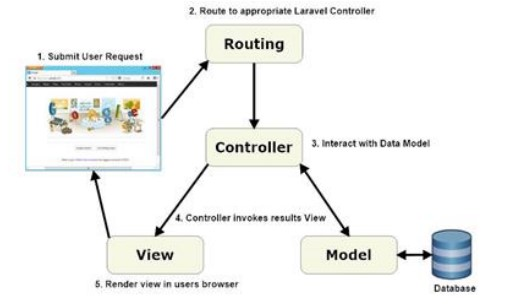
\includegraphics[width=0.9\textwidth]
	{pics/ilustrasimvc.jpg}
	\caption{Illustrasi MVC}
	\label{fig:31}
\end{figure}

Terdapat 5 konsep arsitektur pada framework laravel yang masing-masing memiliki fungsi sebagai berikut[7] :

\begin{enumerate}

\item Routes berfungsi untuk memberi akses pada setiap request sesuai alur yang telah di tentukan. Router memiliki 4 instruksi standar, diantaranya :

\begin{enumerate}

\item Get	\hspace{0.47cm}: untuk memanggil request.

\item Put	\hspace{0.51cm}: untuk mengambil data sesuai request.

\item Post	\hspace{0.5cm}: untuk menambahkan data sesuai request.

\item Delete \hspace{0.12cm}: untuk menghapus data sesuai request.
\end{enumerate}

\item Controller merupakan bagian penghubung antara model dan view. Controller memiliki perintah yang berfungsi untuk memproses bagaimana data ditampilkan dari Model ke View atau sebaliknya. Controller memiliki struktur untuk penulisan kode program pada ralavel yaitu :

\begin{enumerate}

\item Index	\hspace{0.34cm}: untuk menampilkan data keseluruhan.

\item Create \hspace{0.2cm}: untuk memanggil form yang berisi kolom inputan.

\item Store	\hspace{0.4cm}: untuk menyimpan data ke dalam table.

\item Show	\hspace{0.35cm}: untuk menampilkan data sesuai dengan ID.

\item Edit	\hspace{0.57cm}: untuk memanggil data sesuai dengan ID yang berisi form    inputan untuk proses update.

\item Update \hspace{0.1cm}: untuk mengudate data pada table.

\item Delete \hspace{0.19cm}: untuk menghapus data sesuai ID.
\end{enumerate}

\item Model yaitu sekumpulan data yang memiliki fungsi untuk mengelola table pada database. Struktur pemodelan data pada ralaver yaitu memiliki fungsi yang terdiri dari table, primaryKey dan fillable. Dimana ketiga fungsi tersebut harus protected. Pada bagian table harus diisi dengan nama table yang sesuai pada database, di bagian primaryKey harus diisi sesuai primaryKey pada table tersebut dan pada bagian fillable diisi dengan bagian-bagian yang mencangkup dalam table tersebut.

\item View adalah file yang berisi kode html (HyperText Markup Language) yang berfungsi untuk menampilkan suatu data ke dalam browser. Format view pada ralavel harus menggunakan istilah blade, contohnya: view.blade.php.

\item Migrations merupakan proses perancangan suatu table, dalam hal ini migrations berfungsi untuk blueprint database atau dapat diistilahkan sebagai penyedia sistem kontrol untuk skema database. 

\end{enumerate}

%-----------------------------------------------------------------------------%
\section{Aplikasi Serupa}
%-----------------------------------------------------------------------------%



\blindtext \\

\begin{table}[h]
	\centering
	\caption{Perbandingan Aplikasi Serupa}
	\label{tab:1}
	\begin{tabular}{ c c c }
		\hline
		\textbf{Penulis} 		& \textbf{Aplikasi}  & \textbf{Fitur yang ditawarkan}\\ \hline \hline
		\cite{Narayana2010} 	& Aplikasi-A		& n and p \\ 
		\cite{Patel2016} 		& Aplikasi-B		& p and q \\ 
		\cite{Phadte2017} 		& Aplikasi-C		& q and r \\ 
		\cite{Rachmawanto2017} 	& Aplikasi-D		& r and s \\ 
		\cite{Reddy2016} 		& Aplikasi-E		& s and t \\ \hline
	\end{tabular}
\end{table}

% Bab 3 : Perancangan
%---------------------------------------------------------------
\chapter{\babTiga}
%---------------------------------------------------------------

%-----------------------------------------------------------------------------%
\section{Sistem Arsitektur}
%-----------------------------------------------------------------------------%

Perancangan sistem arsitektur aplikasi sistem pengawakan jabatan struktural dapat dilihat pada \textbf{Gambar 3.1.} berikut : 

\begin{figure}
	\centering
	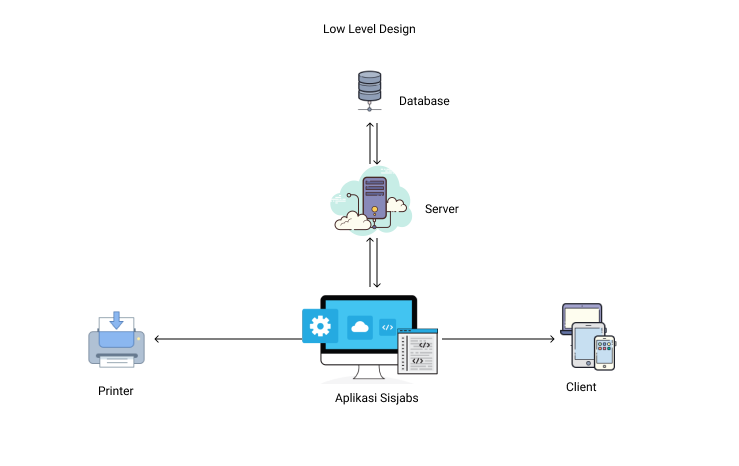
\includegraphics[width=1\textwidth]
	{pics/LowLevelDiagram.png}
	\caption{Low Level Design}
	\label{fig:31}
\end{figure}


\subsection{Gambaran Umum Sistem}

Aplikasi \textbf{SiPJabS : Sistem Pengawakan Jabatan Struktural di Univertias Telkom} merupakan aplikasi berbasis web yang memudahkan bagi perusahaan dalam pencarian seorang kandidat atau posisi yang kosong. Dalam pembuatan aplikasi ini dibutuhkan fitur \textit{filtering} yang digunakan untuk pencarian kandidat baru, yang sesuai dengan ketentuan yang sudah ditetapkan oleh perusahaan. Sistem \textit{filtering} dapat dilakukan setiap saat, untuk menggantikan pekerjaan lama yang telah berhenti dikarenakan pensiun, meninggal, mengundurkan diri atau diberhentikan karena suatu kebijakan tertentu. \\

Data-data pegawai yang berada di Universitas Telkom dapat dilihat dan data tersebut bersifat rahasia. Sehingga aplikasi ”\textbf{SiPJabS : Sistem Pengawakan Jabatan Struktural di Universitas Telkom}” hanya dapat diakses oleh orang tertentu. Aplikasi ini terdapat satu \textit{user} yang dapat mengelola proses \textit{filtering} dan satu \textit{admin} yang mengelola infrastruktur \textit{database} dan proyek \textit{server} serta jaringan.  

Sistem \textit{filtering} pada apliaksi ini terbagi menjadi dua bagian, yang pertama merupakan \textit{fitering} secara umum dengan isi \textit{form} seperti jabatan minimal dan masa kerja. Yang kedua merupakan \textit{filtering} secara khusus, dimana \textit{user} dapat mencari kandidat dengan syarat yang lebih spesifik lagi untuk dijadikan pilihan, kemudian akan terdapat beberapa nama kandidat, apabila sudah menentukan pilihan dapat menekan tombol button pada nama yang akan dipilih dan akan masuk dalam \textit{cart} kandidat.

Apabila proses pencarian kandidat sudah ditemukan dengan salah satu proses \textit{filtering} yang sudah dijelaskan diatas maka, proses selanjutnya akan masuk dalam pembuatan berita acara dan dapat dicetak berupa file pdf.  

\subsection{Target Pengguna Aplikasi}

Aplikasi \textbf{SiPJabS} memiliki beberapa target pengguna diantaranya sebagai berikut :

\begin{enumerate}
\item User \\
User merupakan pegawai Direktorat Sumber Daya Manusia Universitas Telkom yang membutuhkan kandidat dengan proses \textit{filtering} untuk mengisi posisi yang kosong atau digantikan.

\item Admin \\
Admin merupakan pegawai Direktorat Pusat Teknologi Informasi Universitas Telkom yang mengelola dan menyediakan data untuk proses filtering.
\end{enumerate}

\subsection{Spesifikasi Target Perangkat}

Spesifikasi dari target perangkat untuk mengakses aplikasi SiPJabS adalah sebagai berikut : 

\begin{enumerate}

\item Komputer atau laptop yang terhubung dengan koneksi internet dan dapat membuka \textit{browser}.

\item	\textit{Smartphone} atau tablet yang terhubung dengan koneksi internet dan dapat membuka \textit{browser}.
\end{enumerate}

\subsection{Diagram Alir Aplikasi}

Dalam membangun aplikasi SiPJabS, dibutuhkan diagram alir untuk membantu developer dan pengguna dalam memahami sistem yang akan dibuat. Berikut merupakan flowchart :

\begin{figure}
	\centering
	\includegraphics[width=1\textwidth]
	{pics/diagram/flowchart.png}
	\caption{Flowchart}
	\label{fig:31}
\end{figure}  

\newpage
%-----------------------------------------------------------------------------%
\section{Kebutuhan Pengembangan Sistem}
%-----------------------------------------------------------------------------%

Dalam membangun aplikasi \textbf{SiPJabS}, dibutuhkan beberapa perangkat untuk mengimplementasikannya. Perangkat tersebut dibagi menjadi tiga, yaitu perangkat keras (hardware), perangkat lunak (software) dan hosting. Adapun kebutuhan pengembangan sistem adalah sebagai berikut : 

\subsection{Kubutuhan Perangkat Keras (Hardware) }

\textit{Hardware} yang dibutuhkan dalam perancangan dan pembuatan aplikasi SiPJabs
adalah sebagai berikut :


\begin{table}[H]
	\centering
	\caption{Tabel Kebutuhan Hardware}
	\begin{tabular}{ | c | l | p{75mm} | }
		\hline
		No. & Perangkat Keras & Spesifikasi \\
		\hline
		\multirow{6}{*}{1} & \multirow{6}{*}{Laptop MSI GL62M} & Processor : Intel Core i7-7700HQ \\
		& & Operating sistem : Windows 10 Education \\
		& & RAM : 8 GB \\
		& & Storage : 128 GB SSD + 1 TB Hardisk \\
		& & Graphics Card :  nVidia Geforce GTX 1050 \\
		& & Display : 15.6" FHD, Anti-Glare (1920 x 1080) \\
		
		
		\hline
		
		\multirow{6}{*}{2} & \multirow{6}{*}{Laptop HP Pavilion x360} & Processor : Intel Core i3-6100U \\
		& & Operating sistem : Windows 10 Home \\
		& & RAM : 12 GB \\
		& & Storage : 500 GB Hardisk\\
		& & Graphics Card : Intel HD 520 Graphics \\
		& & Display : 13.3" HD, Touch Screen \\
		
		\hline
	\end{tabular}
\end{table}


\newpage
\subsection{Kebutuhkan Perangkat Lunak (Software)}

\textit{Software} yang dibutuhkan dalam perancangan dan pembuatan aplikasi SiPJabs
adalah sebagai berikut :

\begin{table}[H]
	\centering
	\caption{Tabel Kebutuhan Software}
	\begin{tabular}{ | c | l | p{65mm} | }
		\hline
		No. & Perangkat Lunak & Kegunaan \\
		\hline
		
		1 & Visual Studio Code & Text editor untuk menuliskan \textit{coding} aplikasi \\
				
		\hline
		
		2 & XAMPP & Sebagai server yang berdiri sendiri, yang terdiri atas program Apache HTTP Server, MySQL database, dan penerjemah bahasa yang ditulis dengan bahasa pemrograman PHP dan Perl \\
		
		\hline
		
		3 & IBM Rational System Architect  & Sebuah software untuk mendesain rancangan sistem aplikasi \\
		
		\hline
		
		4 & Figma & Untuk mendesai user interface secara online \\
		
		
		\hline
		
		5 & Microsoft Office Word & Untuk membuat dokumen dan laporan \\
		
		\hline
		
		6 & TexStudio & Untuk membuat laporan dalam latex \\
		
		\hline
		
		7 & Adobe Premier Pro & Editing vidio demo dan vidio promosi \\
		
		\hline
		
		8 & Brave dan Mozila Firefox & Web browser \\
		
		\hline
	\end{tabular}
\end{table}

\subsection{Kebutuhan Hosting}

\textit{Hosting} yang dibutuhkan dalam perancangan dan pembuatan aplikasi SiPJabs
adalah sebagai berikut :

\begin{table}[H]
	\centering
	\caption{Tabel Kebutuhan Hosting}
	\begin{tabular}{ | c | l | l | }
		\hline
		No. & Server & Spesifikasi \\
		\hline
		\multirow{5}{*}{1} & \multirow{5}{*}{Server Indonesia} & Storage : 2 GB \\
		& & RAM : 1 GB \\
		& & Bandwith : Unlimited \\
		& & Processor : 1 Core \\
		& & Domain : my.id  \\
	
		\hline
	\end{tabular}
\end{table}

%-----------------------------------------------------------------------------%
\section{Perancangan Model Program}
%-----------------------------------------------------------------------------%
Perancangan model program dalam pembuatan aplikasi SiPJabS antara
lain Use Case Diagram, Use Case Skenario, Class Diagram,
Entity Relationship Diagram (ERD). Adapun perancangan model program adalah sebagai berikut :

\subsection{Use Case Diagram}

\begin{figure}
	\centering
	\includegraphics[width=1\textwidth]
	{pics/diagram/usecase.png}
	\caption{Use Case Diagram}
	\label{fig:32}
\end{figure}


\subsection{Use Case Skenario}
Berikut merupakan use case scenario dalam pembuatan aplikasi SiPJabS :

\begin{enumerate}
	\item Skenario Login
	
	Nomor \kern 3.6pc : SP-01 \\
	Nama Use Case : Melakukan login \\
	Aktor \kern 4.1 pc : Admin \\
	Tipe \kern 4.6pc : Primary \\
	Tujuan \kern 3.6pc : Penggunaan aplikasi \\
	Deskripsi \kern 2.5pc : 
	
	\begin{itemize}
		\item Admin dapat menginputkan username dan password
		\item Sistem akan mencocokkan data
		\item Sistem menampilkan halaman utama aplikasi
	\end{itemize}

	\begin{table}
		\caption{Skenario Login}
		\centering
		\begin{tabular}{ | p{55mm} | p{60mm} |}
			\hline 
			\textbf{Aktor} & \textbf{Sistem} \\
			\hline
			
			1.	Menginputkan username dan password &  \\
			
			\hline
			
			& 2. Mencocokkan data \\
			
			\hline
			
			& 3.	Menampilkan halaman utama aplikasi \\
		
			\hline
			
		\end{tabular}
	\end{table}

\item Skenario Edit Profile

Nomor \kern 3.6pc : SP-02 \\
Nama Use Case : Melakukan edit profile \\
Aktor \kern 4.1 pc : Admin \\
Tipe \kern 4.6pc : Primary \\
Tujuan \kern 3.6pc : Admin dapat melakukan edit pada profile \\
Deskripsi \kern 2.5pc : 

\begin{itemize}
	\item Admin menuju ke halaman profile
	\item Sistem akan menampilkan halaman profile
	\item Admin memilih edit profile
	\item Sistem menampilkan pop-up form edit profile
	\item Admin menginputkan data
	\item Admin menyimpan perubahan

\end{itemize}

\begin{table}
	\caption{Skenario Edit Profile}
	\centering
	\begin{tabular}{ | l | l |}
		\hline 
		\textbf{Aktor} & \textbf{Sistem} \\
		\hline
		
		1.	Menuju ke halaman profile &  \\
		
		\hline
		
		&  2.	Menampilkan halaman profile \\
		
		\hline
		
		 3. Memilih edit profile & \\
		
		\hline
		
			& 4.	Menampilkan pop-up form edit profile \\
		
		\hline
		
		5.	Menginputkan data  & \\
		\hline
		
		6.	Menyimpan perubahan & \\
		\hline
		
		& 7.	Menyimpan perubahan \\
		\hline
		
	\end{tabular}
\end{table}

\item Skenario Reset Password

Nomor \kern 3.6pc : SP-03 \\
Nama Use Case : Melakukan reset password \\
Aktor \kern 4.1 pc : Admin \\
Tipe \kern 4.6pc : Primary \\
Tujuan \kern 3.6pc : Admin dapat melakukan reset password pada profile \\
Deskripsi \kern 2.5pc : 

\begin{itemize}
	\item Admin menuju ke halaman profile
	\item Sistem akan menampilkan halaman profile
	\item Admin memilih reset password
	\item Sistem menampilkan pop-up reset password
	\item Admin menginputkan password
	\item Admin menyimpan perubahan
	\item Sistem menyimpan perubahan
	
\end{itemize}

\begin{table}
	\caption{Skenario Reset Password}
	\centering
	\begin{tabular}{ | l | l |}
		\hline 
		\textbf{Aktor} & \textbf{Sistem} \\
		\hline
		
		1.	Menuju ke halaman profile &  \\
		
		\hline
		
		&  2.	Menampilkan halaman profile \\
		
		\hline
		
		3. Memilih reset password & \\
		
		\hline
		
		& 4.	Menampilkan pop-up reset password \\
		
		\hline
		
		5.	Menginputkan password  & \\
		\hline
		
		6.	Menyimpan perubahan & \\
		\hline
		
		& 7.	Menyimpan perubahan \\
		\hline
		
	\end{tabular}
\end{table}

\item Skenario Tambah Users

Nomor \kern 3.6pc : SP-04 \\
Nama Use Case : Menambahkan users \\
Aktor \kern 4.1 pc : Admin \\
Tipe \kern 4.6pc : Primary \\
Tujuan \kern 3.6pc : Admin dapat menambahkan users \\
Deskripsi \kern 2.5pc : 

\begin{itemize}
	\item Admin menuju ke halaman data users
	\item Sistem akan menampilkan halaman data users
	\item Admin memilih tambah users
	\item Sistem menampilkan halaman form tambah userd
	\item Admin menginputkan data
	\item Admin menyimpan data
	\item Sistem menyimpan data
	\item Sistem menampilkan pop-up tanda berhasil ditambahkan user
	
\end{itemize}

\begin{table}
	\caption{Skenario Tambah Users}
	\centering
	\begin{tabular}{ | l | p{65mm} |}
		\hline 
		\textbf{Aktor} & \textbf{Sistem} \\
		\hline
		
		1.	Menuju ke halaman data users &  \\
		
		\hline
		
		&  2.	Menampilkan halaman data users \\
		
		\hline
		
		3. Memilih tambah users & \\
		
		\hline
		
		& 4.	Menampilkan halaman form tambah users \\
		
		\hline
		
		5.	Menginputkan data  & \\
		\hline
		
		6.	Menyimpan data & \\
		\hline
		
		& 7.	Menyimpan perubahan \\
		\hline
		
		& 8.	Menampilkan pop-up tanda berhasil menambahkan user \\
		\hline
		
	\end{tabular}
\end{table}

\newpage
\item Skenario Edit Users

Nomor \kern 3.6pc : SP-05 \\
Nama Use Case : Melakukan edit data users \\
Aktor \kern 4.1 pc : Admin \\
Tipe \kern 4.6pc : Primary \\
Tujuan \kern 3.6pc : Admin dapat edit data users \\
Deskripsi \kern 2.5pc : 

\begin{itemize}
	\item Admin menuju ke halaman data users
	\item Sistem akan menampilkan halaman data users
	\item Admin memilih edit pada salah satu users
	\item Sistem menampilkan pop-up edit profile
	\item Admin menginputkan data
	\item Admin menyimpan data
	\item Sistem menyimpan data
	\item Sistem menampilkan pop-up tanda berhasil pengubahan data
	
\end{itemize}

\begin{table}
	\caption{Skenario Edit Users}
	\centering
	\begin{tabular}{ | l | p{65mm} |}
		\hline 
		\textbf{Aktor} & \textbf{Sistem} \\
		\hline
		
		1.	Menuju ke halaman data users &  \\
		
		\hline
		
		&  2.	Menampilkan halaman data users \\
		
		\hline
		
		3. Memilih edit pada salah satu users & \\
		
		\hline
		
		& 4.	Menampilkan pop-up form edit users \\
		
		\hline
		
		5.	Menginputkan data  & \\
		\hline
		
		6.	Menyimpan data & \\
		\hline
		
		& 7.	Menyimpan perubahan \\
		\hline
		
		& 8.	Menampilkan pop-up tanda berhasil mengubah user \\
		\hline
		
	\end{tabular}
\end{table}

\item Skenario Delete Users

Nomor \kern 3.6pc : SP-06 \\
Nama Use Case : Melakukan delete data users \\
Aktor \kern 4.1 pc : Admin \\
Tipe \kern 4.6pc : Primary \\
Tujuan \kern 3.6pc : Admin dapat delete data users \\
Deskripsi \kern 2.5pc : 

\begin{itemize}
	\item Admin menuju ke halaman data users
	\item Sistem akan menampilkan halaman data users
	\item Admin memilih delete pada salah satu users
	\item Sistem menampilkan pop-up tanda berhasil hapus data
	
\end{itemize}

\begin{table}
	\caption{Skenario Delete Users}
	\centering
	\begin{tabular}{ | l | p{65mm} |}
		\hline 
		\textbf{Aktor} & \textbf{Sistem} \\
		\hline
		
		1.	Menuju ke halaman data users &  \\
		
		\hline
		
		&  2.	Menampilkan halaman data users \\
		
		\hline
		
		3. Memilih delete pada salah satu users & \\
		
		\hline
		
		& 4.	Menampilkan pop-up tanda berhasil delete data \\
		
		\hline
		
	\end{tabular}
\end{table}

\item Skenario View Data Pegawai

Nomor \kern 3.6pc : SP-07 \\
Nama Use Case : Melakukan view data pegawai \\
Aktor \kern 4.1 pc : Admin \\
Tipe \kern 4.6pc : Primary \\
Tujuan \kern 3.6pc : Admin dapat melihat data pegawai \\
Deskripsi \kern 2.5pc : 

\begin{itemize}
	\item Admin menuju ke halaman data pegawai
	\item Sistem akan menampilkan halaman data pegawai
	\item Admin memilih view pada salah satu pegawai
	\item Sistem menampilkan detail pegawai
	\item Admin dapat melihat data detail pegawai
	
\end{itemize}

\begin{table}
	\caption{Skenario View Data Pegawai}
	\centering
	\begin{tabular}{ | l | p{55mm} |}
		\hline 
		\textbf{Aktor} & \textbf{Sistem} \\
		\hline
		
		1.	Menuju ke halaman data pegawai &  \\
		
		\hline
		
		&  2.	Menampilkan halaman data pegawai \\
		
		\hline
		
		3. Memilih view pada salah satu pegawai & \\
		
		\hline
		
		& 4.	Menampilkan pop-up data detail pegawai \\
		
		\hline
		
		5.	Admin dapat melihat data detail pegawai  & \\
		\hline
		
		
	\end{tabular}
\end{table}

\item Skenario View Data Tallent

Nomor \kern 3.6pc : SP-08 \\
Nama Use Case : Melakukan view data tallent \\
Aktor \kern 4.1 pc : Admin \\
Tipe \kern 4.6pc : Primary \\
Tujuan \kern 3.6pc : Admin dapat melihat data tallent \\
Deskripsi \kern 2.5pc : 

\begin{itemize}
	\item Admin menuju ke halaman data tallent
	\item Sistem akan menampilkan halaman data tallent
	\item Admin memilih view pada salah satu data tallent
	\item Sistem menampilkan detail talent
	\item Admin dapat melihat data detail tallent
	
\end{itemize}

\begin{table}
	\caption{Skenario View Data Tallent}
	\centering
	\begin{tabular}{ |  p{50mm} | p{70mm} |}
		\hline 
		\textbf{Aktor} & \textbf{Sistem} \\
		\hline
		
		1.	Menuju ke halaman data tallent &  \\
		
		\hline
		
		&  2.	Menampilkan halaman data tallent \\
		
		\hline
		
		3. Memilih view pada salah satu data tallent & \\
		
		\hline
		
		& 4.	Menampilkan pop-up data detail tallent \\
		
		\hline
		
		5.	Admin dapat melihat data detail tallent  & \\
		\hline
		
		
	\end{tabular}
\end{table}

\newpage
\item Skenario Print Data Tallent

Nomor \kern 3.6pc : SP-09 \\
Nama Use Case : Melakukan print data tallent \\
Aktor \kern 4.1 pc : Admin \\
Tipe \kern 4.6pc : Primary \\
Tujuan \kern 3.6pc : Admin dapat mencetak data tallent \\
Deskripsi \kern 2.5pc : 

\begin{itemize}
	\item Admin menuju ke halaman data tallent
	\item Sistem akan menampilkan halaman data tallent
	\item Admin memilih print pada salah satu data tallent
	\item Sistem mendownload file data tallent
	
\end{itemize}

\begin{table}
	\caption{Skenario Print Data Tallent}
	\centering
	\begin{tabular}{ | p{50mm} | p{70mm} |}
		\hline 
		\textbf{Aktor} & \textbf{Sistem} \\
		\hline
		
		1.	Menuju ke halaman data tallent &  \\
		
		\hline
		
		&  2.	Menampilkan halaman data tallent \\
		
		\hline
		
		3. Memilih print pada salah satu data tallent & \\
		
		\hline
		
		& 4.	Mendownload data tallent \\
		
		\hline
		
	\end{tabular}
\end{table}

\item Skenario Tambah Unit Kerja

Nomor \kern 3.6pc : SP-10 \\
Nama Use Case : Menambahkan data unit kerja \\
Aktor \kern 4.1 pc : Admin \\
Tipe \kern 4.6pc : Primary \\
Tujuan \kern 3.6pc : Admin dapat menambahkan data unit kerja \\
Deskripsi \kern 2.5pc : 

\begin{itemize}
	\item Admin menuju ke halaman data unit kerja
	\item Sistem akan menampilkan halaman data unit kerja
	\item Admin memilih tambah unit kerja
	\item Sistem menampilkan pop-up tambah unit kerja
	\item Admin menginputkan data
	\item Sistem menyimpan data
	\item Sistem menampilkan pop-up tanda berhasil ditambahkan
	
\end{itemize}

\begin{table}
	\caption{Skenario Tambah Unit Kerja}
	\centering
	\begin{tabular}{ | l | p{65mm} |}
		\hline 
		\textbf{Aktor} & \textbf{Sistem} \\
		\hline
		
		1.	Menuju ke halaman data unit kerja &  \\
		
		\hline
		
		&  2.	Menampilkan halaman data unit kerja \\
		
		\hline
		
		3. Memilih tambah unit kerja & \\
		
		\hline
		
		& 4.	Menampilkan pop-up tambah unit kerja \\
		
		\hline
		
		5.	Menginputkan data  & \\
		\hline
		
		& 6.	Menyimpan data \\
		\hline
		
		& 7.	Menampilkan pop-up tanda berhasil menambahkan data \\
		\hline
		
	\end{tabular}
\end{table}

\item Skenario Edit Unit Kerja

Nomor \kern 3.6pc : SP-11 \\
Nama Use Case : Mengubah data unit kerja \\
Aktor \kern 4.1 pc : Admin \\
Tipe \kern 4.6pc : Primary \\
Tujuan \kern 3.6pc : Admin dapat mengubah data unit kerja \\
Deskripsi \kern 2.5pc : 

\begin{itemize}
	\item Admin menuju ke halaman data unit kerja
	\item Sistem akan menampilkan halaman data unit kerja
	\item Admin memilih edit pada suatu data unit kerja
	\item Sistem menampilkan pop-up edit unit kerja
	\item Admin menginputkan data
	\item Sistem menyimpan data
	\item Sistem menampilkan pop-up tanda berhasil di edit
	
\end{itemize}

\begin{table}
	\caption{Skenario Edit Unit Kerja}
	\centering
	\begin{tabular}{ | p{55mm} | p{70mm} |}
		\hline 
		\textbf{Aktor} & \textbf{Sistem} \\
		\hline
		
		1.	Menuju ke halaman data unit kerja &  \\
		
		\hline
		
		&  2.	Menampilkan halaman data unit kerja \\
		
		\hline
		
		3. Memilih edit pada suatu data unit kerja & \\
		
		\hline
		
		& 4.	Menampilkan pop-up edit unit kerja \\
		
		\hline
		
		5.	Menginputkan data  & \\
		\hline
		
		& 6.	Menyimpan data \\
		\hline
		
		& 7.	Menampilkan pop-up tanda berhasil edit data \\
		\hline
		
	\end{tabular}
\end{table}

\item Skenario Delete Unit Kerja

Nomor \kern 3.6pc : SP-12 \\
Nama Use Case : Menghaous data unit kerja \\
Aktor \kern 4.1 pc : Admin \\
Tipe \kern 4.6pc : Primary \\
Tujuan \kern 3.6pc : Admin dapat menghapus data unit kerja \\
Deskripsi \kern 2.5pc : 

\begin{itemize}
	\item Admin menuju ke halaman data unit kerja
	\item Sistem akan menampilkan halaman data unit kerja
	\item Admin memilih delete pada suatu data unit kerja
	\item Sistem menampilkan pop-up tanda berhasil di hapus
	
\end{itemize}

\begin{table}
	\caption{Skenario Delete Unit Kerja}
	\centering
	\begin{tabular}{ | p{55mm} | p{70mm} |}
		\hline 
		\textbf{Aktor} & \textbf{Sistem} \\
		\hline
		
		1.	Menuju ke halaman data unit kerja &  \\
		
		\hline
		
		&  2.	Menampilkan halaman data unit kerja \\
		
		\hline
		
		3. Memilih delete pada suatu data unit kerja & \\
		
		\hline
		
		& 4.	Menampilkan pop-up tanda berhasil delete data \\
		\hline
		
	\end{tabular}
\end{table}

\newpage
\item Skenario Tambah Jabatan

Nomor \kern 3.6pc : SP-13 \\
Nama Use Case : Menambahkan data jabatan \\
Aktor \kern 4.1 pc : Admin \\
Tipe \kern 4.6pc : Primary \\
Tujuan \kern 3.6pc : Admin dapat menambahkan data jabatan \\
Deskripsi \kern 2.5pc : 

\begin{itemize}
	\item Admin menuju ke halaman data jabatan
	\item Sistem akan menampilkan halaman data jabatan
	\item Admin memilih tambah jabatan
	\item Sistem menampilkan pop-up tambah jabatan
	\item Admin menginputkan data
	\item Sistem menyimpan data
	\item Sistem menampilkan pop-up tanda berhasil ditambahkan
	
\end{itemize}

\begin{table}
	\caption{Skenario Tambah Jabatan}
	\centering
	\begin{tabular}{ | l | p{65mm} |}
		\hline 
		\textbf{Aktor} & \textbf{Sistem} \\
		\hline
		
		1.	Menuju ke halaman data jabatan &  \\
		
		\hline
		
		&  2.	Menampilkan halaman data jabatan \\
		
		\hline
		
		3. Memilih tambah jabatan & \\
		
		\hline
		
		& 4.	Menampilkan pop-up tambah jabatan \\
		
		\hline
		
		5.	Menginputkan data  & \\
		\hline
		
		& 6.	Menyimpan data \\
		\hline
		
		& 7.	Menampilkan pop-up tanda berhasil menambahkan data \\
		\hline
		
	\end{tabular}
\end{table}

\item Skenario Edit Jabatan

Nomor \kern 3.6pc : SP-14 \\
Nama Use Case : Mengubah data jabatan \\
Aktor \kern 4.1 pc : Admin \\
Tipe \kern 4.6pc : Primary \\
Tujuan \kern 3.6pc : Admin dapat mengubah data jabatan \\
Deskripsi \kern 2.5pc : 

\begin{itemize}
	\item Admin menuju ke halaman data jabatan
	\item Sistem akan menampilkan halaman data jabatan
	\item Admin memilih edit pada suatu data jabatan
	\item Sistem menampilkan pop-up edit jabatan
	\item Admin menginputkan data
	\item Sistem menyimpan data
	\item Sistem menampilkan pop-up tanda berhasil di edit
	
\end{itemize}

\begin{table}
	\caption{Skenario Edit Jabatan}
	\centering
	\begin{tabular}{ | l | p{65mm} |}
		\hline 
		\textbf{Aktor} & \textbf{Sistem} \\
		\hline
		
		1.	Menuju ke halaman data jabatan &  \\
		
		\hline
		
		&  2.	Menampilkan halaman data jabatan \\
		
		\hline
		
		3. Memilih edit pada suatu data jabatan & \\
		
		\hline
		
		& 4.	Menampilkan pop-up edit jabatan \\
		
		\hline
		
		5.	Menginputkan data  & \\
		\hline
		
		& 6.	Menyimpan data \\
		\hline
		
		& 7.	Menampilkan pop-up tanda berhasil edit data \\
		\hline
		
	\end{tabular}
\end{table}

\item Skenario Delete Jabatan

Nomor \kern 3.6pc : SP-15 \\
Nama Use Case : Menghaous data jabatan \\
Aktor \kern 4.1 pc : Admin \\
Tipe \kern 4.6pc : Primary \\
Tujuan \kern 3.6pc : Admin dapat menghapus data jabatan \\
Deskripsi \kern 2.5pc : 

\begin{itemize}
	\item Admin menuju ke halaman data jabatan
	\item Sistem akan menampilkan halaman data jabatan
	\item Admin memilih delete pada suatu data jabatan
	\item Sistem menampilkan pop-up tanda berhasil di hapus
	
\end{itemize}

\begin{table}
	\caption{Skenario Delete Jabatan}
	\centering
	\begin{tabular}{ | p{55mm} | p{70mm}|}
		\hline 
		\textbf{Aktor} & \textbf{Sistem} \\
		\hline
		
		1.	Menuju ke halaman data jabatan &  \\
		
		\hline
		
		&  2.	Menampilkan halaman data jabatan \\
		
		\hline
		
		3. Memilih delete pada suatu data jabatan & \\
		
		\hline
		
		& 4.	Menampilkan pop-up tanda berhasil delete data \\
		\hline
		
	\end{tabular}
\end{table}

\item Skenario Tambah Unit Bagian

Nomor \kern 3.6pc : SP-16 \\
Nama Use Case : Menambahkan data unit bagian \\
Aktor \kern 4.1 pc : Admin \\
Tipe \kern 4.6pc : Primary \\
Tujuan \kern 3.6pc : Admin dapat menambahkan data unit bagian \\
Deskripsi \kern 2.5pc : 

\begin{itemize}
	\item Admin menuju ke halaman data unit bagian
	\item Sistem akan menampilkan halaman data unit bagian
	\item Admin memilih tambah unit bagian
	\item Sistem menampilkan pop-up tambah unit bagian
	\item Admin menginputkan data
	\item Sistem menyimpan data
	\item Sistem menampilkan pop-up tanda berhasil ditambahkan
	
\end{itemize}

\begin{table}
	\caption{Skenario Tambah Unit Bagian}
	\centering
	\begin{tabular}{ | p{55mm} | p{70mm} |}
		\hline 
		\textbf{Aktor} & \textbf{Sistem} \\
		\hline
		
		1.	Menuju ke halaman data unit bagian &  \\
		
		\hline
		
		&  2.	Menampilkan halaman data unit bagian \\
		
		\hline
		
		3. Memilih tambah unit bagian & \\
		
		\hline
		
		& 4.	Menampilkan pop-up tambah unit bagian \\
		
		\hline
		
		5.	Menginputkan data  & \\
		\hline
		
		& 6.	Menyimpan data \\
		\hline
		
		& 7.	Menampilkan pop-up tanda berhasil menambahkan data \\
		\hline
		
	\end{tabular}
\end{table}

\item Skenario Edit Unit Bagian

Nomor \kern 3.6pc : SP-17 \\
Nama Use Case : Mengubah data unit bagian \\
Aktor \kern 4.1 pc : Admin \\
Tipe \kern 4.6pc : Primary \\
Tujuan \kern 3.6pc : Admin dapat mengubah data unit bagian \\
Deskripsi \kern 2.5pc : 

\begin{itemize}
	\item Admin menuju ke halaman data unit bagian
	\item Sistem akan menampilkan halaman data unit bagian
	\item Admin memilih edit pada suatu data unit bagian
	\item Sistem menampilkan pop-up edit unit bagian
	\item Admin menginputkan data
	\item Sistem menyimpan data
	\item Sistem menampilkan pop-up tanda berhasil di edit
	
\end{itemize}

\begin{table}
	\caption{Skenario Edit Unit Bagian}
	\centering
	\begin{tabular}{ | p{55mm} | p{70mm} |}
		\hline 
		\textbf{Aktor} & \textbf{Sistem} \\
		\hline
		
		1.	Menuju ke halaman data unit bagian &  \\
		
		\hline
		
		&  2.	Menampilkan halaman data unit bagian \\
		
		\hline
		
		3. Memilih edit pada suatu data unit bagian & \\
		
		\hline
		
		& 4.	Menampilkan pop-up edit unit bagian \\
		
		\hline
		
		5.	Menginputkan data  & \\
		\hline
		
		& 6.	Menyimpan data \\
		\hline
		
		& 7.	Menampilkan pop-up tanda berhasil edit data \\
		\hline
		
	\end{tabular}
\end{table}

\item Skenario Delete Unit Bagian

Nomor \kern 3.6pc : SP-18 \\
Nama Use Case : Menghaous data unit bagian \\
Aktor \kern 4.1 pc : Admin \\
Tipe \kern 4.6pc : Primary \\
Tujuan \kern 3.6pc : Admin dapat menghapus data unit bagian \\
Deskripsi \kern 2.5pc : 

\begin{itemize}
	\item Admin menuju ke halaman data unit bagian
	\item Sistem akan menampilkan halaman data unit bagian
	\item Admin memilih delete pada suatu data unit bagian
	\item Sistem menampilkan pop-up tanda berhasil di hapus
	
\end{itemize}

\begin{table}
	\caption{Skenario Delete Unit Bagian}
	\centering
	\begin{tabular}{ | p{55mm} | p{70mm} |}
		\hline 
		\textbf{Aktor} & \textbf{Sistem} \\
		\hline
		
		1.	Menuju ke halaman data unit bagian &  \\
		
		\hline
		
		&  2.	Menampilkan halaman data unit bagian \\
		
		\hline
		
		3. Memilih delete pada suatu data unit bagian & \\
		
		\hline
		
		& 4.	Menampilkan pop-up tanda berhasil delete data \\
		\hline
		
	\end{tabular}
\end{table}

\item Skenario Tambah Jabatan Struktural

Nomor \kern 3.6pc : SP-19 \\
Nama Use Case : Menambahkan data jabatan struktural \\
Aktor \kern 4.1 pc : Admin \\
Tipe \kern 4.6pc : Primary \\
Tujuan \kern 3.6pc : Admin dapat menambahkan data jabatan struktural\\
Deskripsi \kern 2.5pc : 

\begin{itemize}
	\item Admin menuju ke halaman data jabatan struktural
	\item Sistem akan menampilkan halaman data jabatan struktural
	\item Admin memilih tambah jabatan struktural
	\item Sistem menampilkan pop-up tambah jabatan struktural
	\item Admin menginputkan data
	\item Sistem menyimpan data
	\item Sistem menampilkan pop-up tanda berhasil ditambahkan
	
\end{itemize}

\begin{table}
	\caption{Skenario Tambah Jabatan Struktural}
	\centering
	\begin{tabular}{ | p{55mm} | p{70mm} |}
		\hline 
		\textbf{Aktor} & \textbf{Sistem} \\
		\hline
		
		1.	Menuju ke halaman data jabatan struktural &  \\
		
		\hline
		
		&  2.	Menampilkan halaman data jabatan struktural\\
		
		\hline
		
		3. Memilih tambah jabatan struktural& \\
		
		\hline
		
		& 4.	Menampilkan pop-up tambah jabatan struktural\\
		
		\hline
		
		5.	Menginputkan data  & \\
		\hline
		
		& 6.	Menyimpan data \\
		\hline
		
		& 7.	Menampilkan pop-up tanda berhasil menambahkan data \\
		\hline
		
	\end{tabular}
\end{table}

\item Skenario Edit Jabatan Struktural

Nomor \kern 3.6pc : SP-20 \\
Nama Use Case : Mengubah data jabatan struktural \\
Aktor \kern 4.1 pc : Admin \\
Tipe \kern 4.6pc : Primary \\
Tujuan \kern 3.6pc : Admin dapat mengubah data jabatan struktural\\
Deskripsi \kern 2.5pc : 

\begin{itemize}
	\item Admin menuju ke halaman data jabatan struktural
	\item Sistem akan menampilkan halaman data jabatan struktural
	\item Admin memilih edit pada suatu data jabatan struktural
	\item Sistem menampilkan pop-up edit jabatan struktural
	\item Admin menginputkan data
	\item Sistem menyimpan data
	\item Sistem menampilkan pop-up tanda berhasil di edit
	
\end{itemize}

\begin{table}
	\caption{Skenario Edit Jabatan Struktural}
	\centering
	\begin{tabular}{ |p{55mm} | p{70mm} |}
		\hline 
		\textbf{Aktor} & \textbf{Sistem} \\
		\hline
		
		1.	Menuju ke halaman data jabatan struktural &  \\
		
		\hline
		
		&  2.	Menampilkan halaman data jabatan struktural \\
		
		\hline
		
		3. Memilih edit pada suatu data jabatan struktural & \\
		
		\hline
		
		& 4.	Menampilkan pop-up edit jabatan struktural\\
		
		\hline
		
		5.	Menginputkan data  & \\
		\hline
		
		& 6.	Menyimpan data \\
		\hline
		
		& 7.	Menampilkan pop-up tanda berhasil edit data \\
		\hline
		
	\end{tabular}
\end{table}

\item Skenario Delete Jabatan Struktural

Nomor \kern 3.6pc : SP-21 \\
Nama Use Case : Menghaous data jabatan struktural \\
Aktor \kern 4.1 pc : Admin \\
Tipe \kern 4.6pc : Primary \\
Tujuan \kern 3.6pc : Admin dapat menghapus data jabatan struktural\\
Deskripsi \kern 2.5pc : 

\begin{itemize}
	\item Admin menuju ke halaman data jabatan struktural
	\item Sistem akan menampilkan halaman data jabatan struktural
	\item Admin memilih delete pada suatu data jabatan struktural
	\item Sistem menampilkan pop-up tanda berhasil di hapus 
	
\end{itemize}

\begin{table}
	\caption{Skenario Delete Jabatan Struktural}
	\centering
	\begin{tabular}{ | p{55mm} | p{70mm}|}
		\hline 
		\textbf{Aktor} & \textbf{Sistem} \\
		\hline
		
		1.	Menuju ke halaman data jabatan struktural &  \\
		
		\hline
		
		&  2.	Menampilkan halaman data jabatan struktural\\
		
		\hline
		
		3. Memilih delete pada suatu data jabatan struktural& \\
		
		\hline
		
		& 4.	Menampilkan pop-up tanda berhasil delete data \\
		\hline
		
	\end{tabular}
\end{table}

\end{enumerate}

\subsection{Class Diagram}

\begin{figure}
	\centering
	\includegraphics[width=1\textwidth]
	{pics/diagram/classdiagram.png}
	\caption{Class Diagram}
	\label{fig:32}
\end{figure}

\subsection{Enitity Relationship Diagram}

\begin{figure}
	\centering
	\includegraphics[width=1\textwidth]
	{pics/diagram/erd.png}
	\caption{ERD}
	\label{fig:32}
\end{figure}

%-----------------------------------------------------------------------------%
\section{Perancangan Aplikasi}
%-----------------------------------------------------------------------------%
Dalam perancangan aplikasi SiPJabS diperlukan perancangan antar muka dan perancangan design level tinggi. Perancangan antar muka akan menjelaskan gambaran awal  developer sebelum masuk pada bagian front-end.  Sedangkan perancangan design level tinggi berguna untuk mengingatkan developer tentang sistem kerja pada aplikasi yang akan dibuat.


\subsection{Perancangan Antar Muka}
Pada tahap kebutuhan antar muka terdapat gambaran mengenai aplikasi SiPJabS: Sistem Pengawakan Jabatan Struktural, berikut merupakan mockup dari aplikasi SiPJabS yang sudah dibuat.

\subsubsection{Perancangan Antar Muka Admin}

\begin{table}
	\caption{Tabel Perancangan Antar Muka Admin}
	\centering
	\begin{tabular}{ | c | c | p{35mm} |}
		\hline 
		\textbf{No} & \textbf{Gambar} &  \textbf{Keterangan} \\ 
		\hline
		
		1. & \raisebox{-\totalheight}{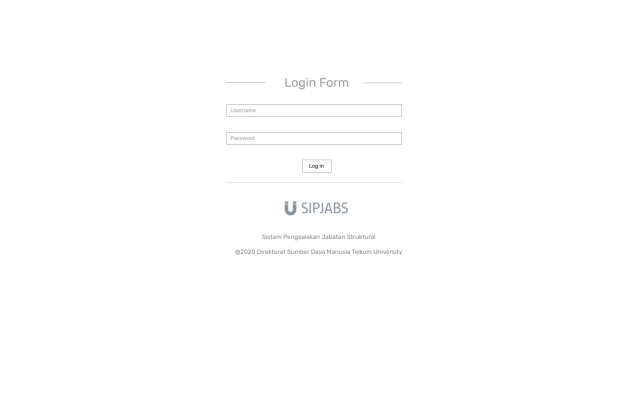
\includegraphics[width=0.6\textwidth, height=60mm]{pics/admin/login.jpg}} 
		& Halaman login merupakan tampilan awal apabila admin membuka aplikasi SiPJabS , admin dapat menginputkan username dan password untuk melakukan login. \\
	
		\hline
		
		2. & \raisebox{-\totalheight}{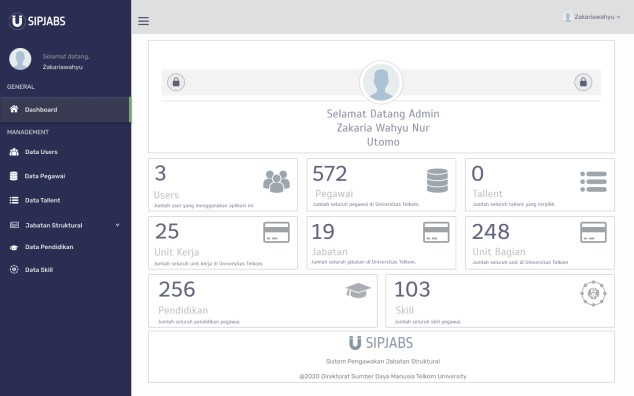
\includegraphics[width=0.6\textwidth, height=60mm]{pics/admin/dashboard.jpg}} 
		& Didalam dashboard admin terdapat jumlah users dari aplikasi SiPJabS, jumlah pegawai di Universitas Telkom, tallent yang sudah dipilih, unit kerja, jabatan, unit bagian, pendidikan dan skill yang dimiliki para pegawai  Universitas Telkom. \\
		\hline

	\end{tabular}
\end{table}


\begin{table}
	\caption{Tabel Perancangan Antar Muka Admin (1)}
	\centering
	\begin{tabular}{ | c | c | p{35mm} |}
		\hline 
		\textbf{No} & \textbf{Gambar} &  \textbf{Keterangan} \\ 
		\hline
		
		3. & \raisebox{-\totalheight}{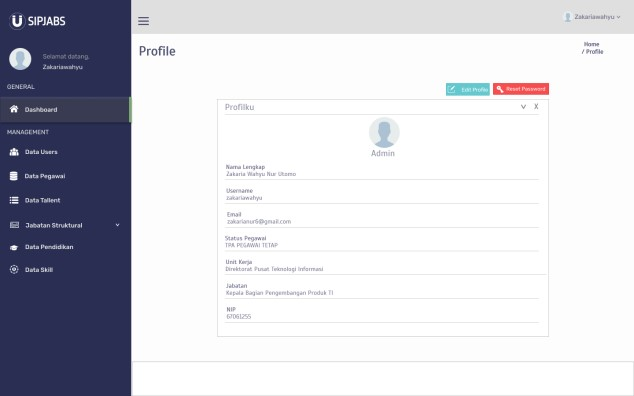
\includegraphics[width=0.6\textwidth, height=60mm]{pics/admin/profile.jpg}} 
		& Halaman profile admin akan menampilkan data profile dari admin tersebut. Kemudian admin juga dapat mengedit profile dan mereset password.  \\
		
		\hline
		
		4. & \raisebox{-\totalheight}{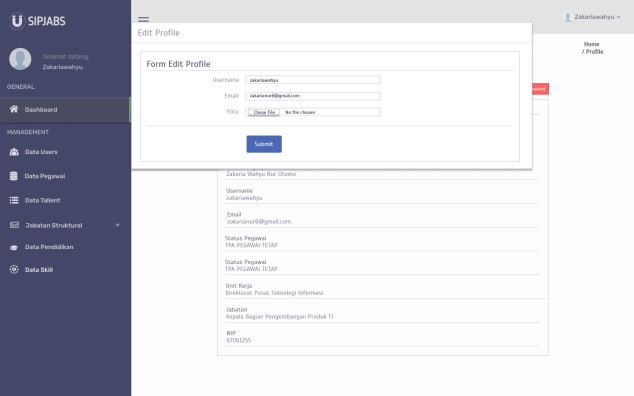
\includegraphics[width=0.6\textwidth, height=60mm]{pics/admin/editprofile.jpg}} 
		& Admin dapat mengubah username, menginputkan email, dan menambahkan foto profile.  \\
		
		\hline
		
		5. & \raisebox{-\totalheight}{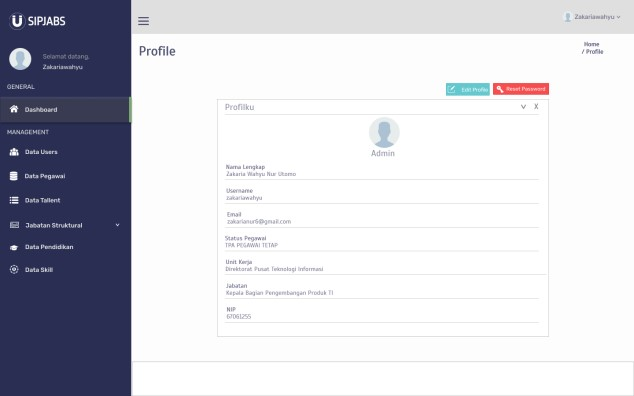
\includegraphics[width=0.6\textwidth, height=60mm]{pics/admin/profile.jpg}} 
		& Halaman profile admin akan menampilkan data dari admin tersebut. Kemudian admin juga dapat mengedit profile dan mereset password. \\
		
		\hline
		
	\end{tabular}
\end{table}

\begin{table}
	\caption{Tabel Perancangan Antar Muka Admin (2)}
	\centering
	\begin{tabular}{ | c | c | p{35mm} |}
		\hline 
		\textbf{No} & \textbf{Gambar} &  \textbf{Keterangan} \\ 
		\hline
		
		6. & \raisebox{-\totalheight}{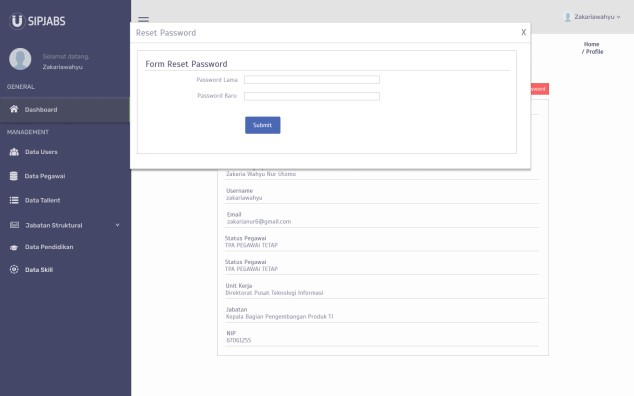
\includegraphics[width=0.6\textwidth, height=60mm]{pics/admin/resetpassword.jpg}} 
		& Admin harus menginputkan password yang lama serta yang baru, setelah itu admin dapat menyimpan. \\
		
		\hline
		
		7. & \raisebox{-\totalheight}{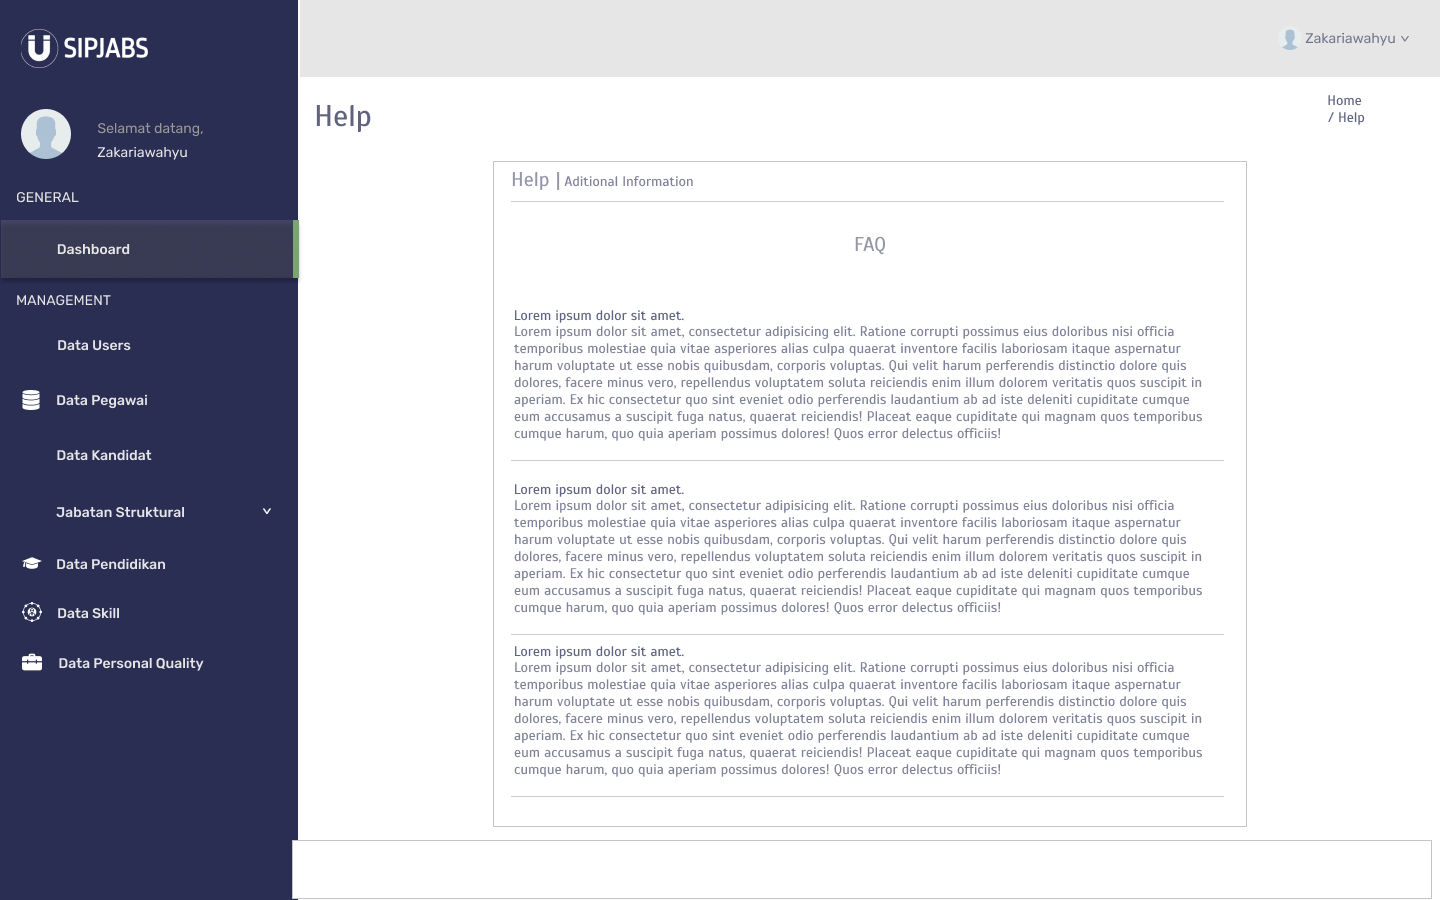
\includegraphics[width=0.6\textwidth, height=60mm]{pics/admin/help.png}} 
		& Halaman help berisi infomasi tentang aplikasi. \\
		
		\hline
		
		8. & \raisebox{-\totalheight}{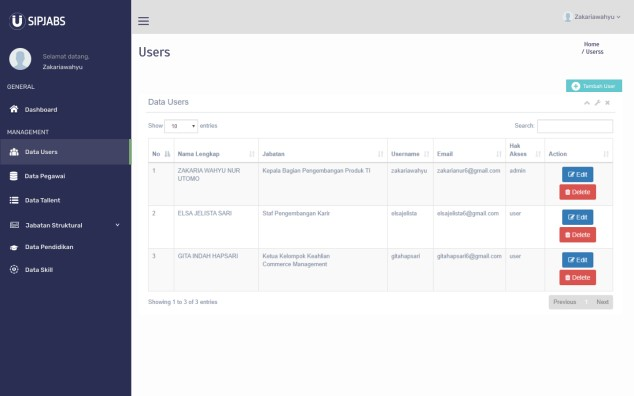
\includegraphics[width=0.6\textwidth, height=60mm]{pics/admin/datausers.jpg}} 
		& Halaman data user akan menampilkan nama-nama yang dapat mengakses aplikasi SiPJabS sebagai admin dan user. \\
		
		\hline
		
	\end{tabular}
\end{table}

\begin{table}
	\caption{Tabel Perancangan Antar Muka Admin (3)}
	\centering
	\begin{tabular}{ | c | c | p{35mm} |}
		\hline 
		\textbf{No} & \textbf{Gambar} &  \textbf{Keterangan} \\ 
		\hline
		
		9. & \raisebox{-\totalheight}{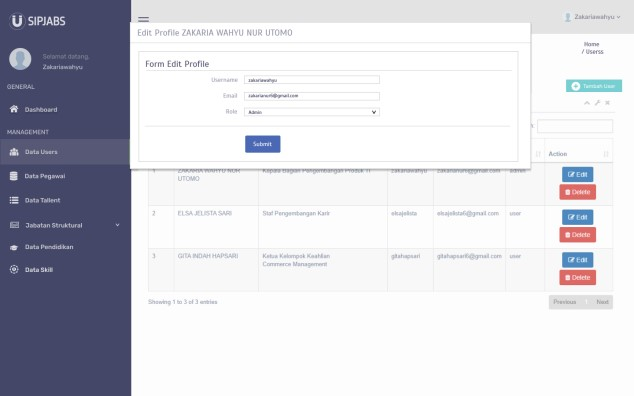
\includegraphics[width=0.6\textwidth, height=60mm]{pics/admin/editdatausers.jpg}} 
		& Pada halaman ini admin dapat mengedit username, email, dan role sebagai admin atau user. \\
		
		\hline
		
		10. & \raisebox{-\totalheight}{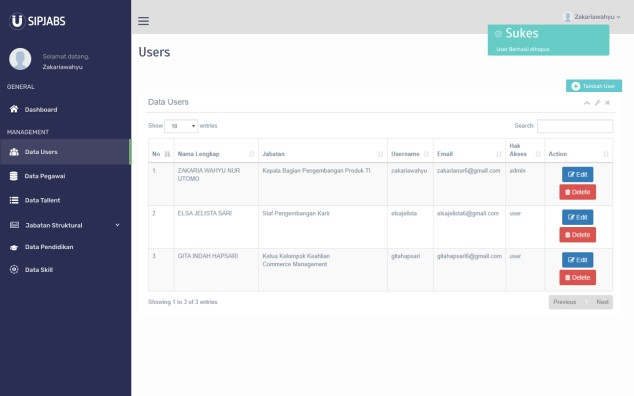
\includegraphics[width=0.6\textwidth, height=60mm]{pics/admin/hapususers.jpg}} 
		&Admin dapat menghapus data user apabila user tersebut sudah tidak bekerja pada bidangnya atau digantikan. \\
		
		\hline
		
		11. & \raisebox{-\totalheight}{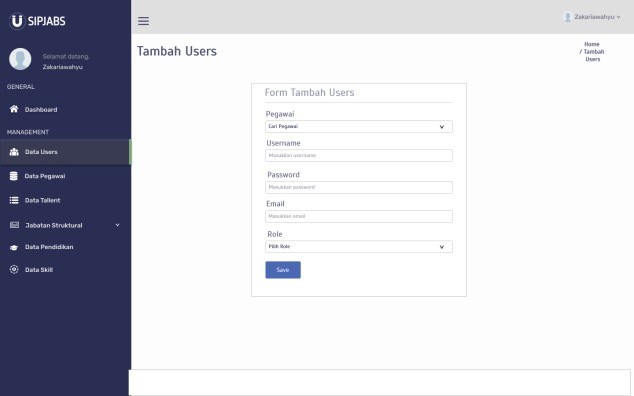
\includegraphics[width=0.6\textwidth, height=60mm]{pics/admin/tambahusers.jpg}} 
		& Admin dapat menambahkan user dengan mengisi form tambah user dan menyimpannya.. \\
		
		\hline
		
	\end{tabular}
\end{table}

\begin{table}
	\caption{Tabel Perancangan Antar Muka Admin (4)}
	\centering
	\begin{tabular}{ | c | c | p{35mm} |}
		\hline 
		\textbf{No} & \textbf{Gambar} &  \textbf{Keterangan} \\ 
		\hline
		
		12. & \raisebox{-\totalheight}{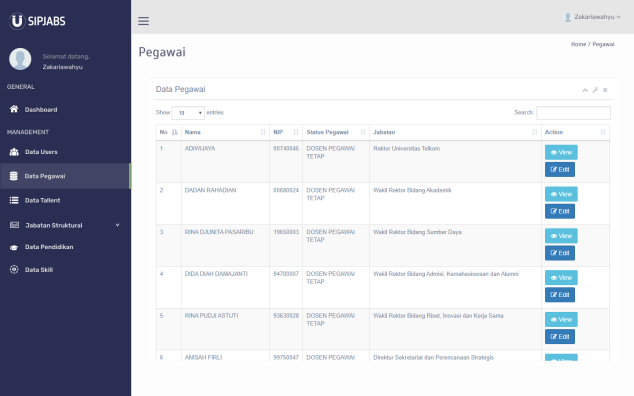
\includegraphics[width=0.6\textwidth, height=60mm]{pics/admin/datapegawai.png}} 
		& Admin dapat melihat daftar data pegawai yang ada di Universitas Telkom secara detail. \\
		
		\hline
		
		13. & \raisebox{-\totalheight}{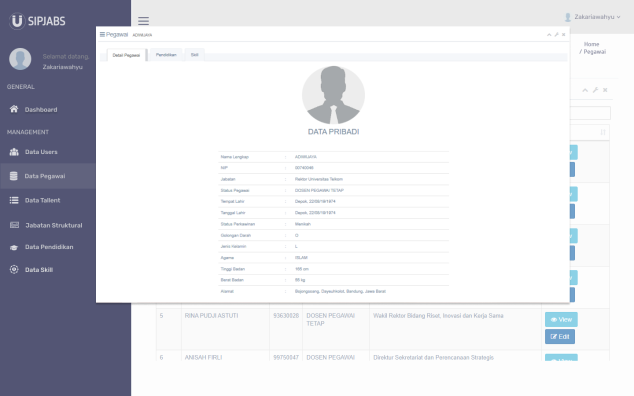
\includegraphics[width=0.6\textwidth, height=60mm]{pics/admin/viewdetailpegawai.png}} 
		&Halaman ini akan menampilkan data pribadi dari pegawai.  \\
		
		\hline
		
		14. & \raisebox{-\totalheight}{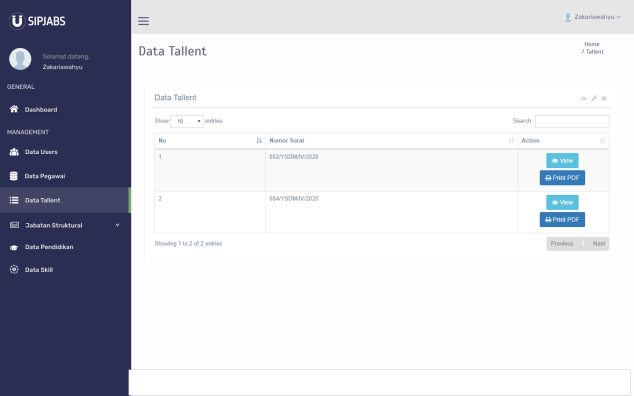
\includegraphics[width=0.6\textwidth, height=60mm]{pics/admin/datatallent.png}} 
		& Halaman ini akan menampilkan data tallent yang sudah di pilih oleh user sesuai dengan job description untuk menggantikan atau mengisi posisi yang kosong. \\
		
		\hline
		
	\end{tabular}
\end{table}

\begin{table}
	\caption{Tabel Perancangan Antar Muka Admin (5)}
	\centering
	\begin{tabular}{ | c | c | p{35mm} |}
		\hline 
		\textbf{No} & \textbf{Gambar} &  \textbf{Keterangan} \\ 
		\hline
		
		15. & \raisebox{-\totalheight}{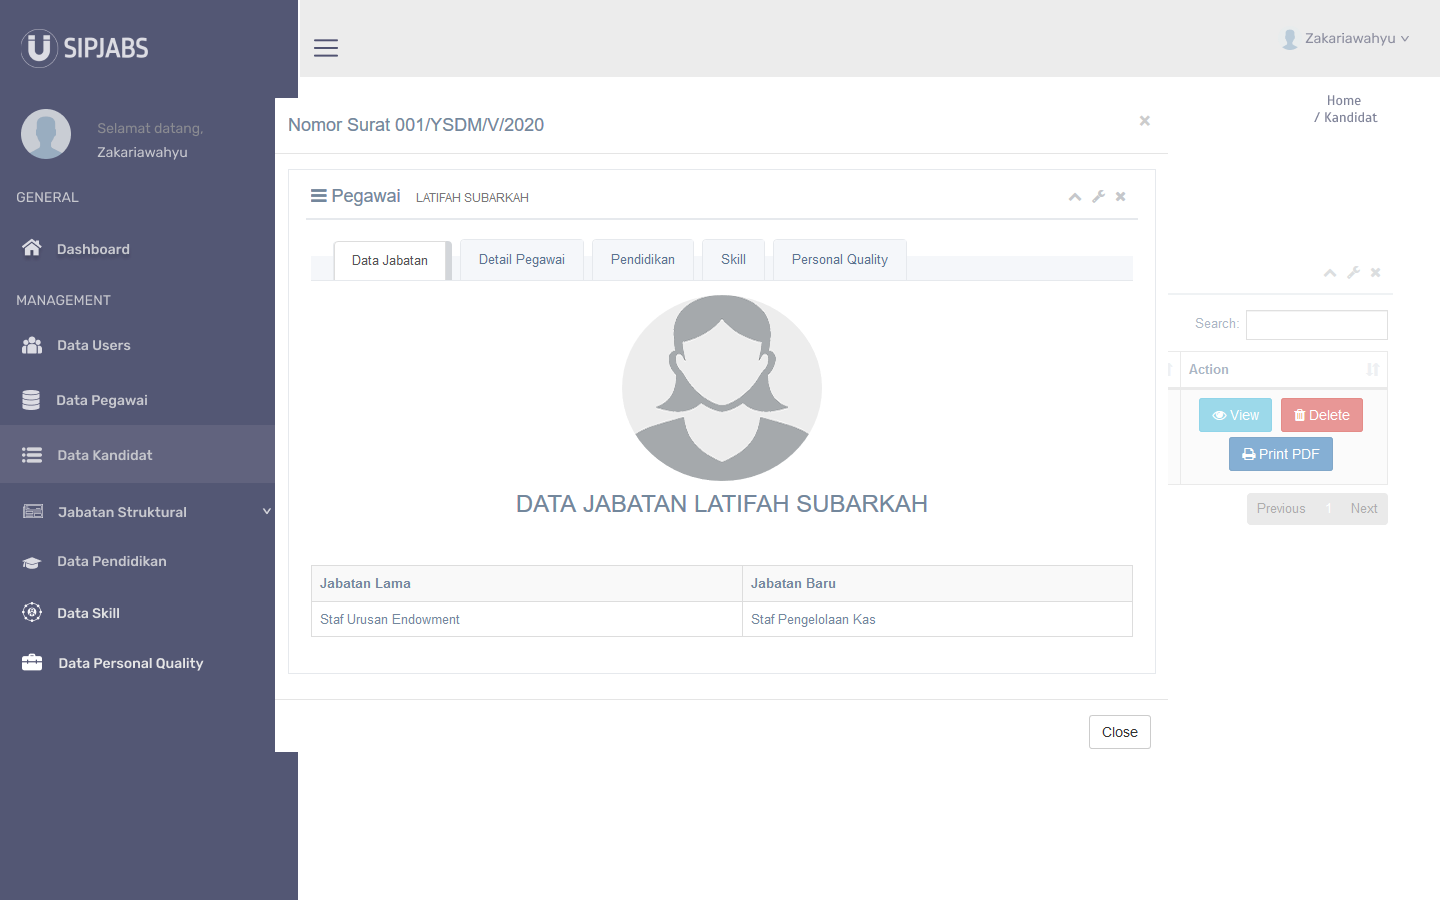
\includegraphics[width=0.6\textwidth, height=60mm]{pics/admin/viewdetailtallent.png}} 
		& Admin dapat melihat data detail tallent yang sudah dipilih. \\
		
		\hline
		
		16. & \raisebox{-\totalheight}{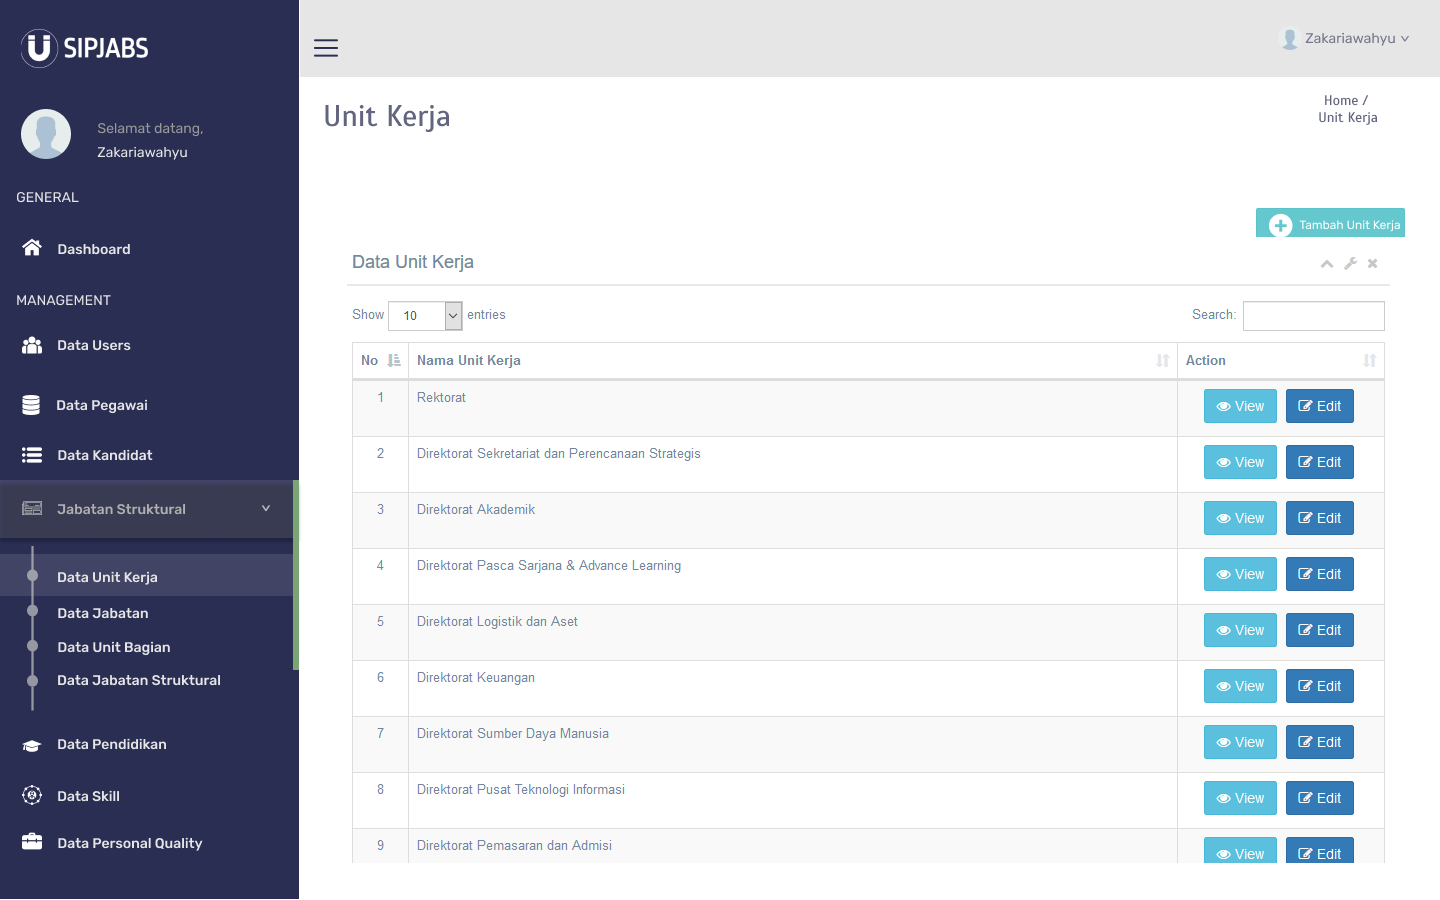
\includegraphics[width=0.6\textwidth, height=60mm]{pics/admin/dataunitkerja.png}} 
		&Halaman ini akan menunjukkan semua unit kerja dimulai dari rektorat hingga fakultas yang ada di Universitas Telkom. \\
		
		\hline
		
		17. & \raisebox{-\totalheight}{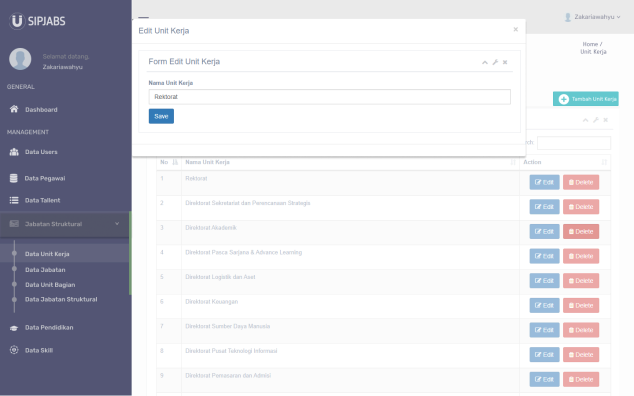
\includegraphics[width=0.6\textwidth, height=60mm]{pics/admin/editunitkerja.png}} 
		& Admin dapat mengedit form unit kerja apabila terdapat kebijakan baru. \\
		
		\hline
		
	\end{tabular}
\end{table}

\begin{table}
	\caption{Tabel Perancangan Antar Muka Admin (6)}
	\centering
	\begin{tabular}{ | c | c | p{35mm} |}
		\hline 
		\textbf{No} & \textbf{Gambar} &  \textbf{Keterangan} \\ 
		\hline
		
		18. & \raisebox{-\totalheight}{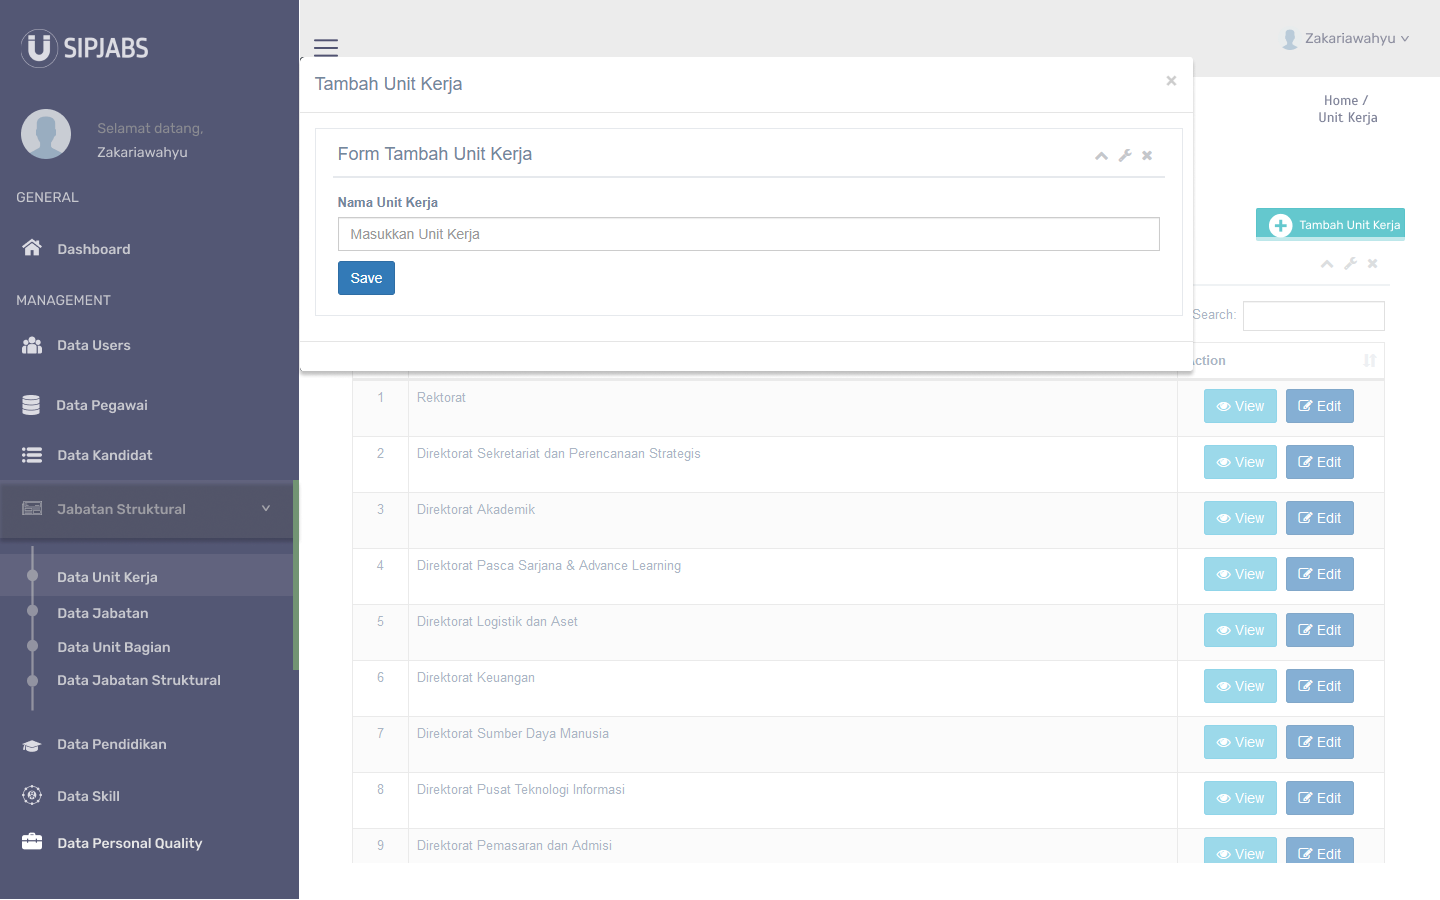
\includegraphics[width=0.6\textwidth, height=60mm]{pics/admin/tambahunitkerja.png}} 
		& Admin dapat menambahkan data unit kerja dengan mengisi form tersebut, namun harus sesuai dengan kebijakan yang telah ditetapkan. \\
		
		\hline
		
		19. & \raisebox{-\totalheight}{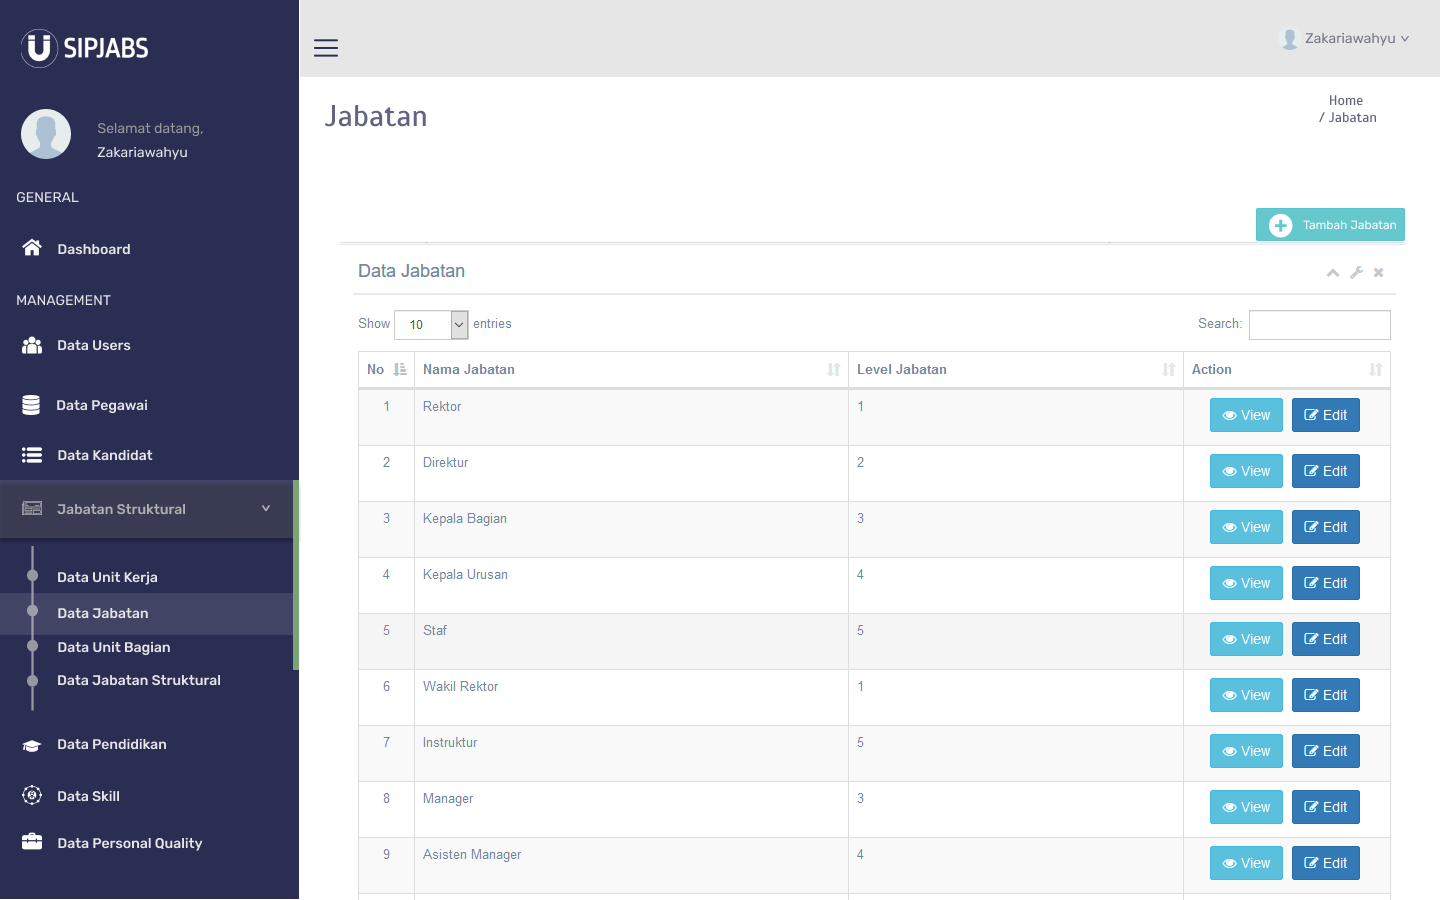
\includegraphics[width=0.6\textwidth, height=60mm]{pics/admin/datajabatan.png}} 
		&Halaman ini akan menampilkan data jabatan yang berada di Universitas Telkom \\
		
		\hline
		
		20. & \raisebox{-\totalheight}{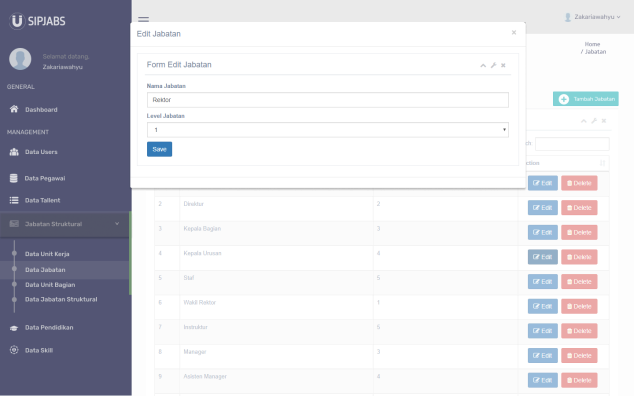
\includegraphics[width=0.6\textwidth, height=60mm]{pics/admin/editjabatan.png}} 
		& Admin dapat mengedit data jabatan sesuai dengan nama jabatan yang sudah ditetapkan. \\
		
		\hline
		
	\end{tabular}
\end{table}

\begin{table}
	\caption{Tabel Perancangan Antar Muka Admin (7)}
	\centering
	\begin{tabular}{ | c | c | p{35mm} |}
		\hline 
		\textbf{No} & \textbf{Gambar} &  \textbf{Keterangan} \\ 
		\hline
		
		21. & \raisebox{-\totalheight}{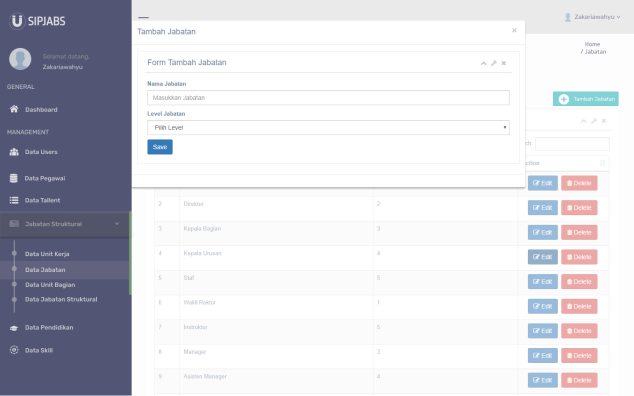
\includegraphics[width=0.6\textwidth, height=60mm]{pics/admin/tambahjabatan.png}} 
		& Admin harus melengkapi form tersebut untuk dapat menambahkan data jabatan yang baru. \\
		
		\hline
		
		22. & \raisebox{-\totalheight}{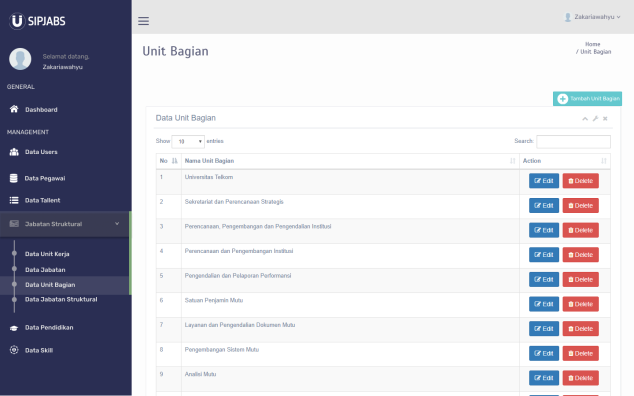
\includegraphics[width=0.6\textwidth, height=60mm]{pics/admin/dataunitbagian.png}} 
		&Halaman ini akan menampilkan satuan kerja yang terdapat di Universitas Telkom.  \\
		
		\hline
		
		23. & \raisebox{-\totalheight}{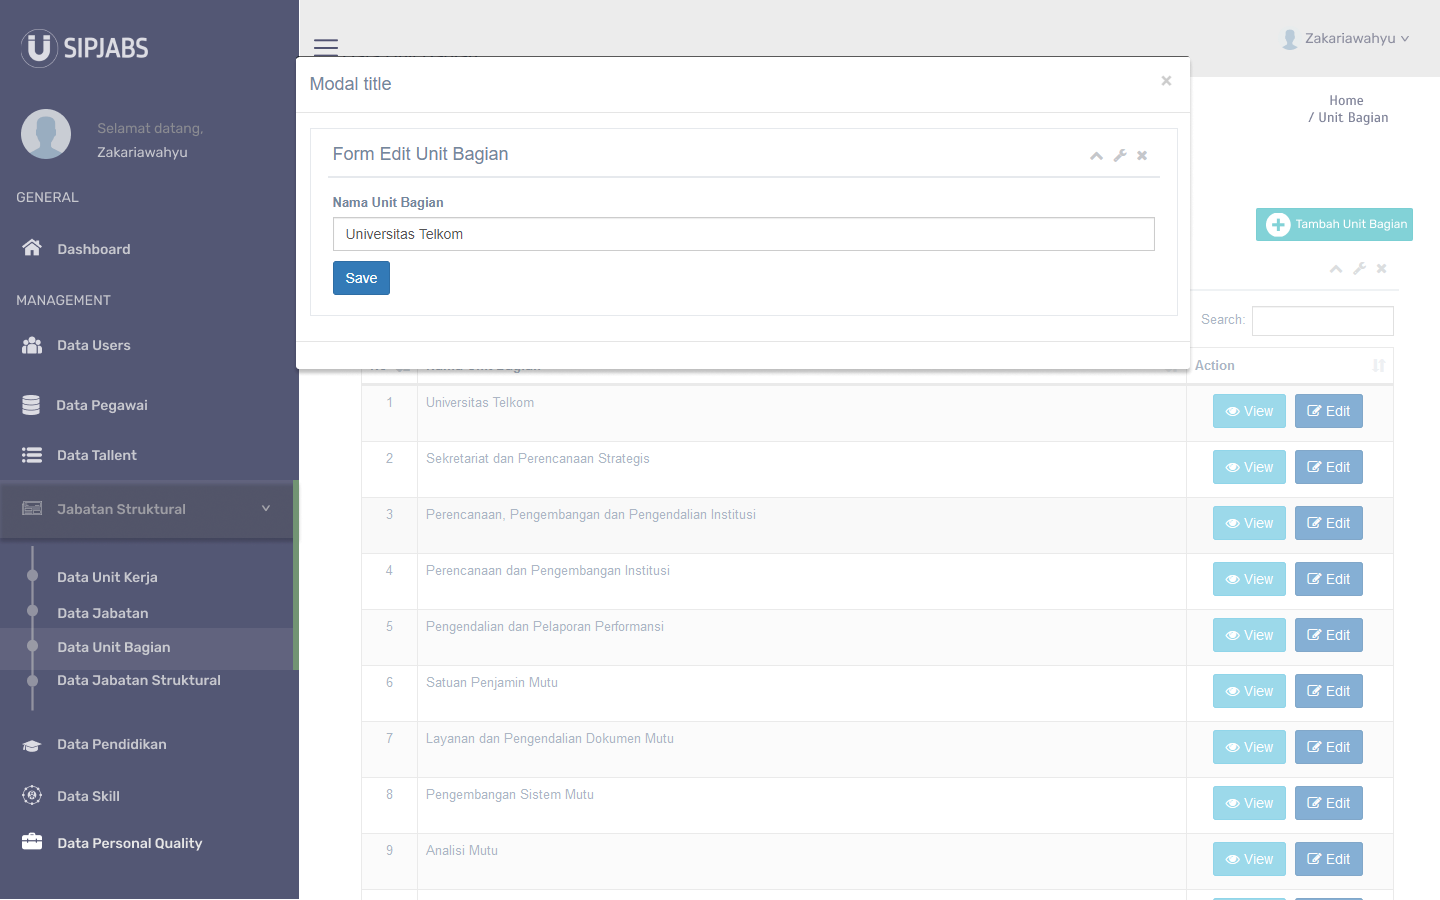
\includegraphics[width=0.6\textwidth, height=60mm]{pics/admin/editunitbagian.png}} 
		& Admin dapat mengedit data unit bagian apabila ada perubahan yang sudah ditetapkan.\\
		
		\hline
		
	\end{tabular}
\end{table}

\begin{table}
	\caption{Tabel Perancangan Antar Muka Admin (8)}
	\centering
	\begin{tabular}{ | c | c | p{35mm} |}
		\hline 
		\textbf{No} & \textbf{Gambar} &  \textbf{Keterangan} \\ 
		\hline
		
		24. & \raisebox{-\totalheight}{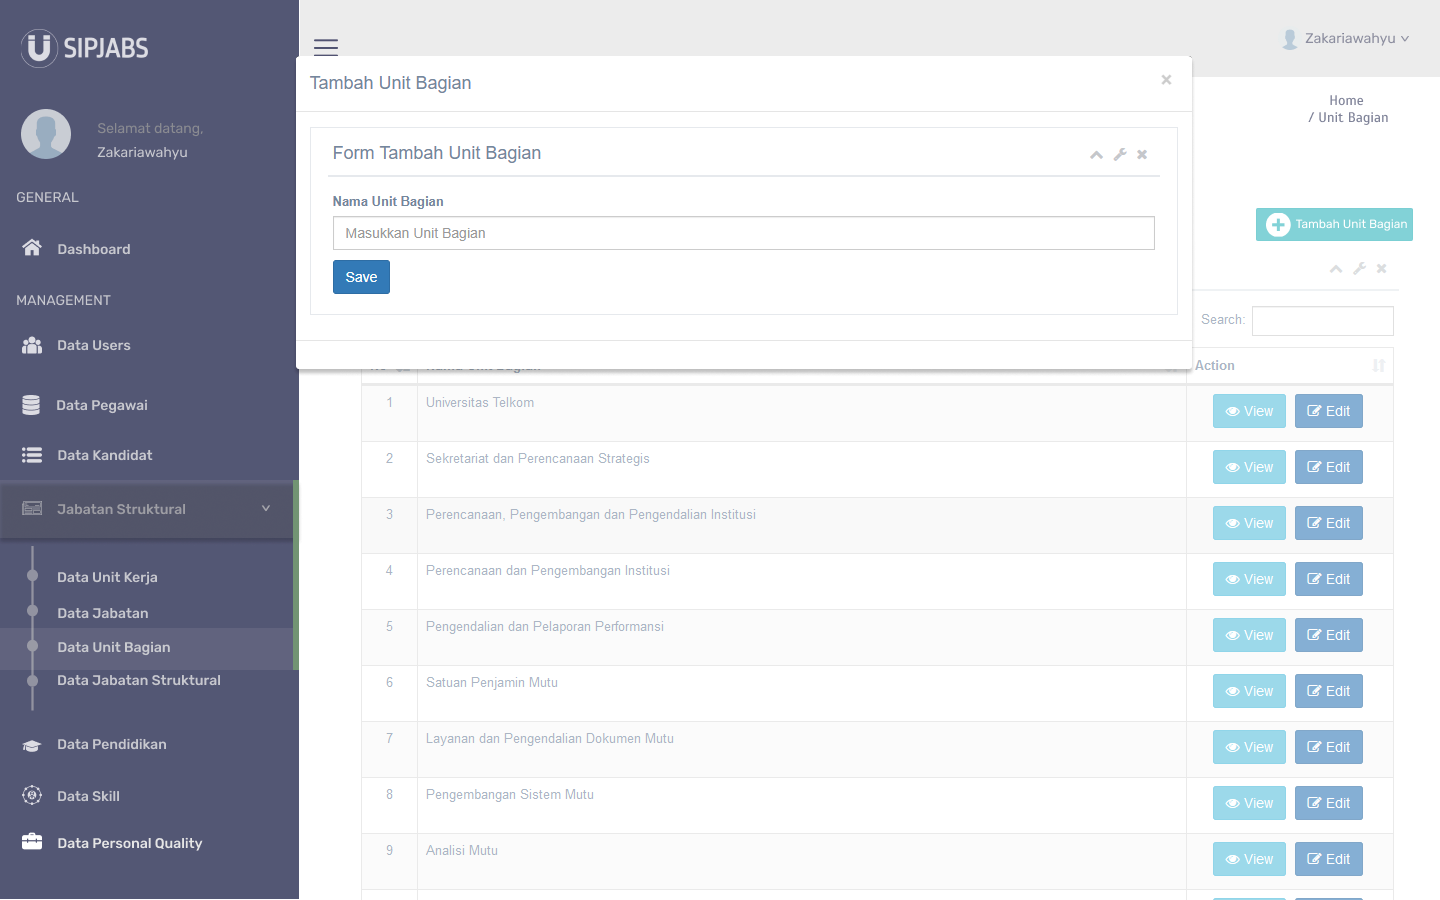
\includegraphics[width=0.6\textwidth, height=60mm]{pics/admin/tambahunitbagian.png}} 
		& Admin harus menginputkan  nama unit bagian  tersebut untuk dapat menambahkan data data unit bagian yang baru. \\
		
		\hline
		
		25. & \raisebox{-\totalheight}{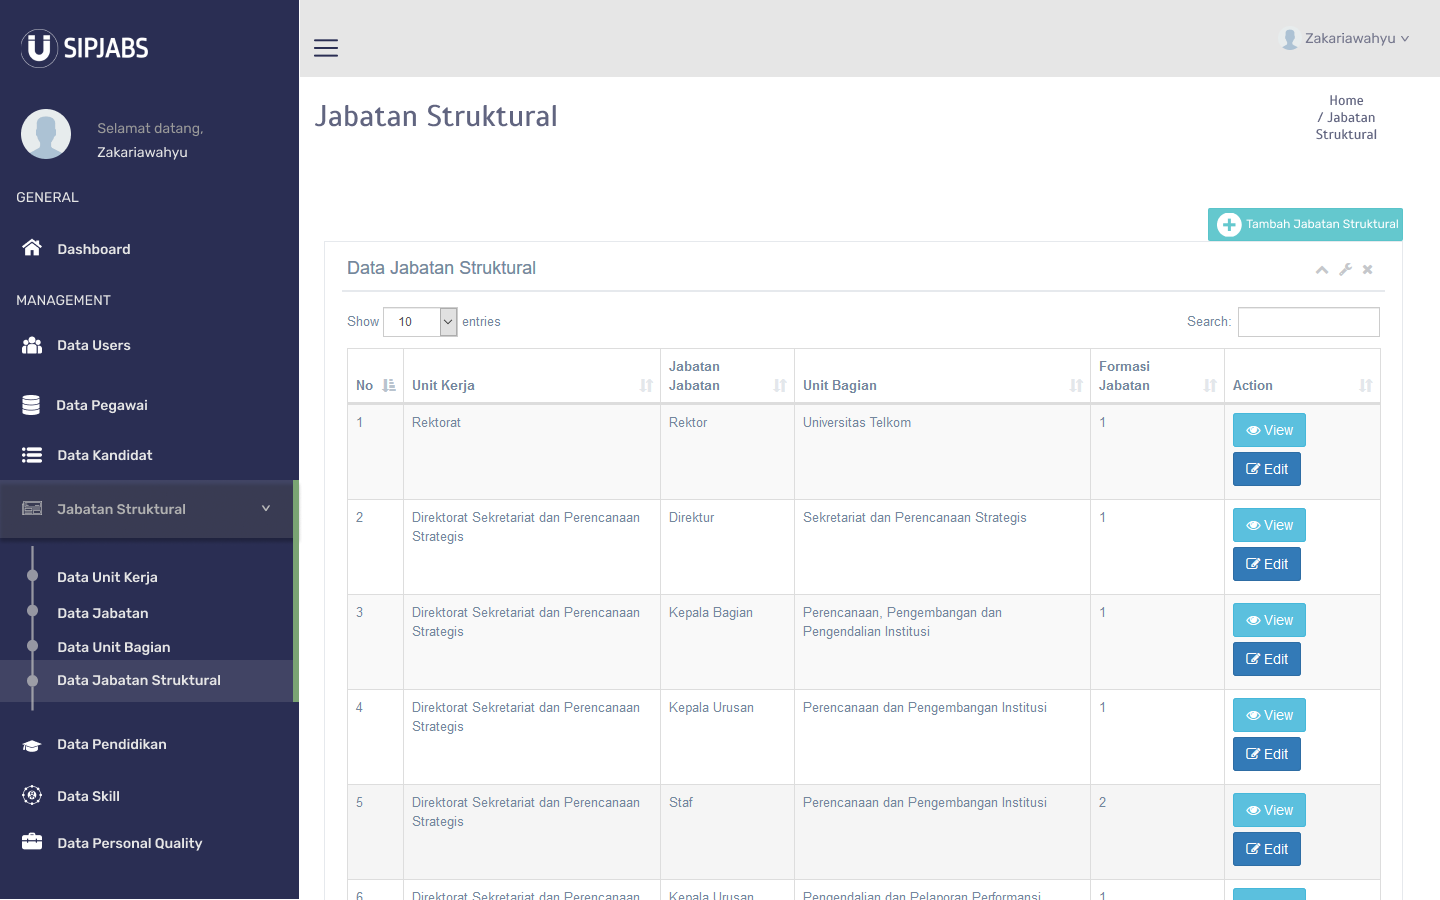
\includegraphics[width=0.6\textwidth, height=60mm]{pics/admin/datajabstruk.png}} 
		&Halaman ini menampilkan jabatan yang secara tegas ada di Universitas Telkom.  \\
		
		\hline
		
		26. & \raisebox{-\totalheight}{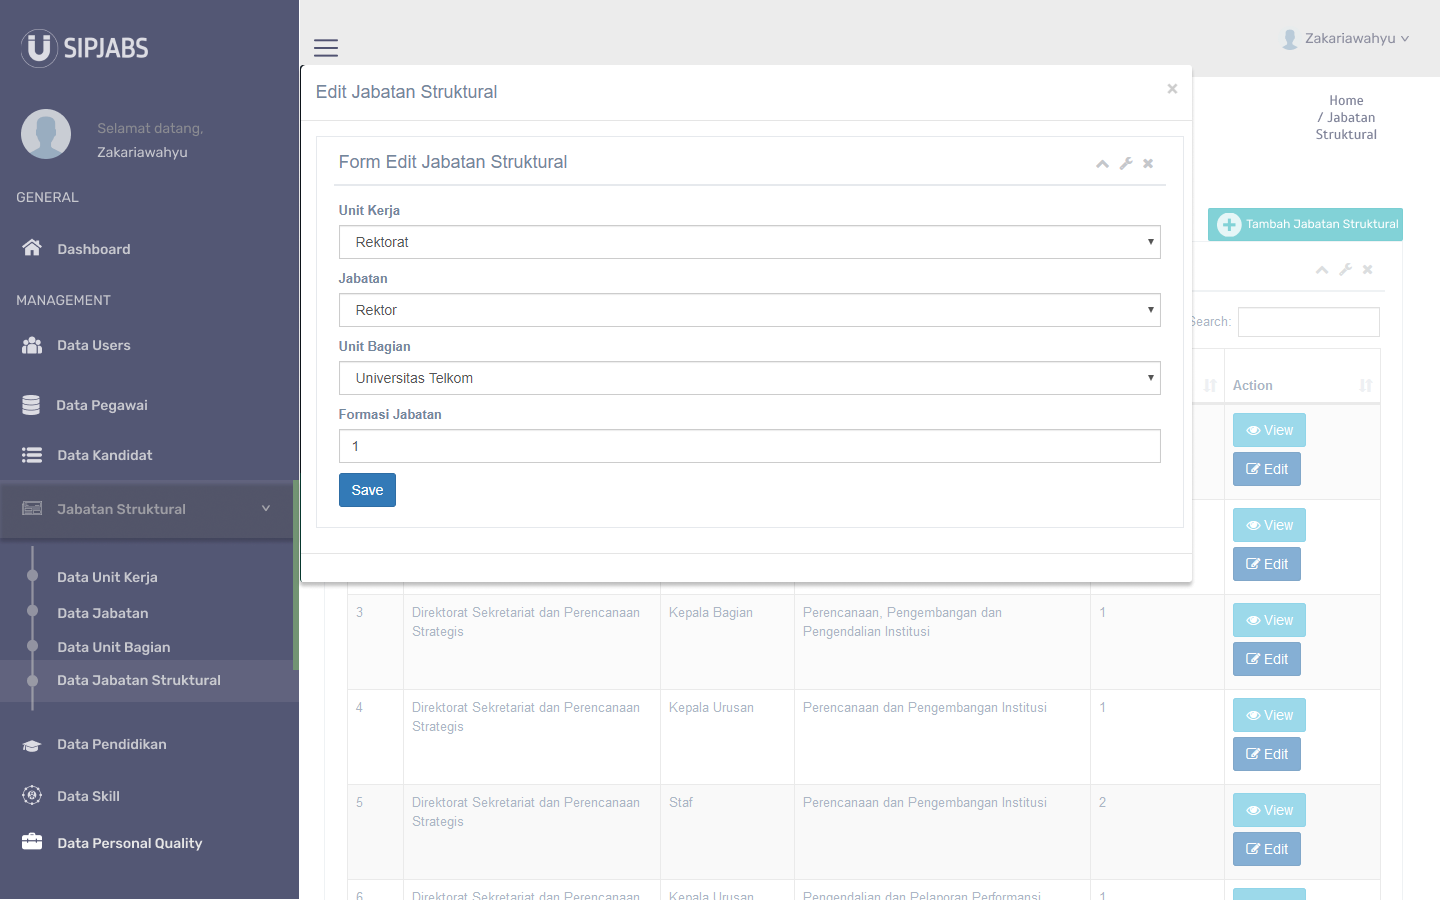
\includegraphics[width=0.6\textwidth, height=60mm]{pics/admin/editjabstruk.png}} 
		& Admin dapat mengedit data dan harus mengisi form sesuai dengan ketetapan.\\
		
		\hline
		
	\end{tabular}
\end{table}

\begin{table}
	\caption{Tabel Perancangan Antar Muka Admin (9)}
	\centering
	\begin{tabular}{ | c | c | p{35mm} |}
		\hline 
		\textbf{No} & \textbf{Gambar} &  \textbf{Keterangan} \\ 
		\hline
		
		27. & \raisebox{-\totalheight}{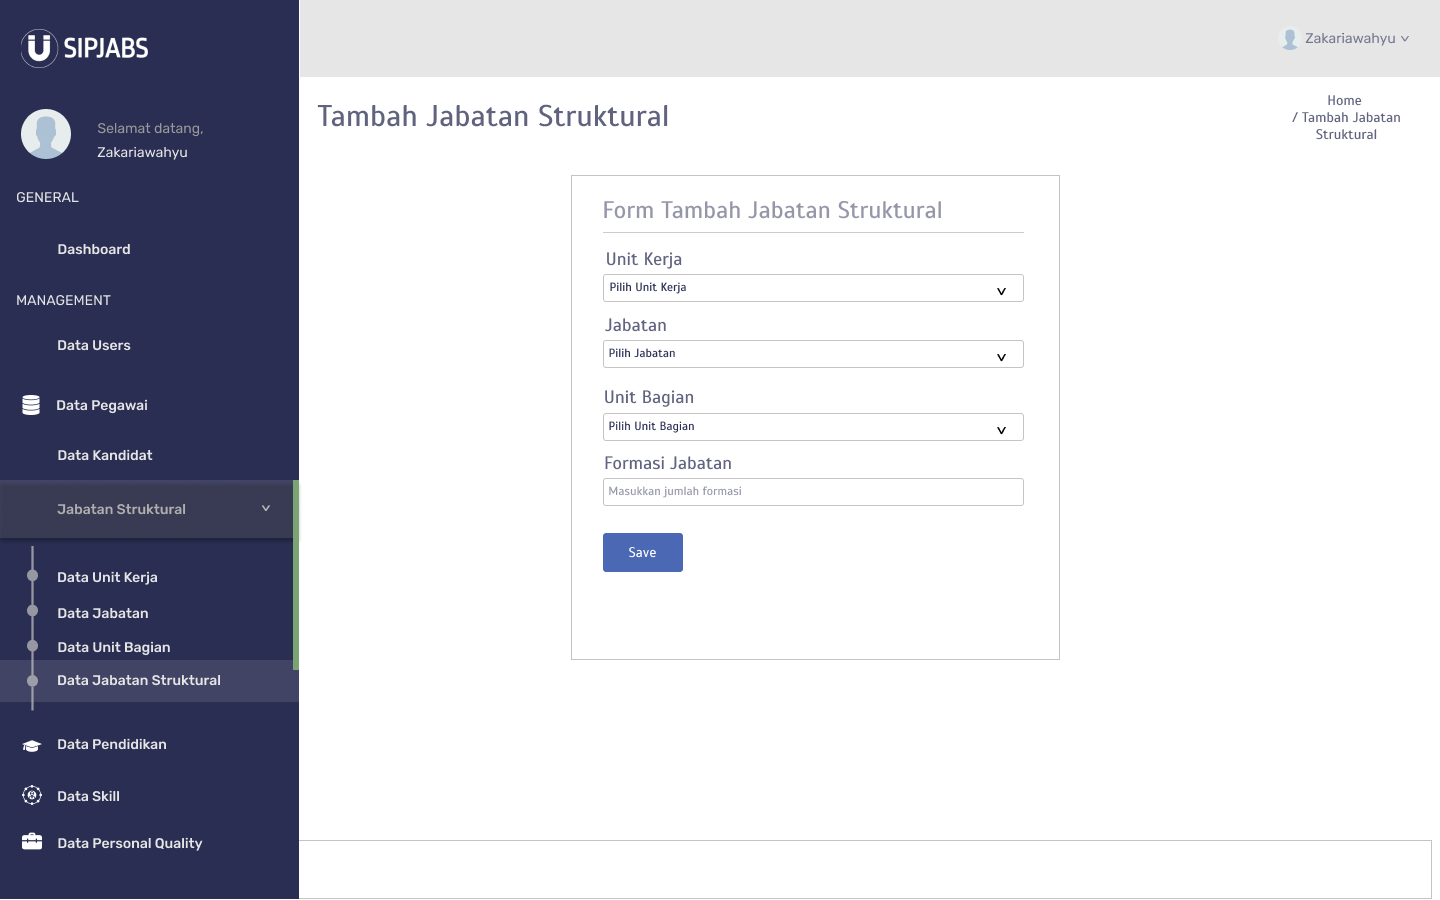
\includegraphics[width=0.6\textwidth, height=60mm]{pics/admin/tambahjabstruk.png}} 
		& Admin harus melengkapi form untuk dapat menambahkan data jabatan struktural baru yang sudah ditetapkan. \\
		
		\hline
		
		28. & \raisebox{-\totalheight}{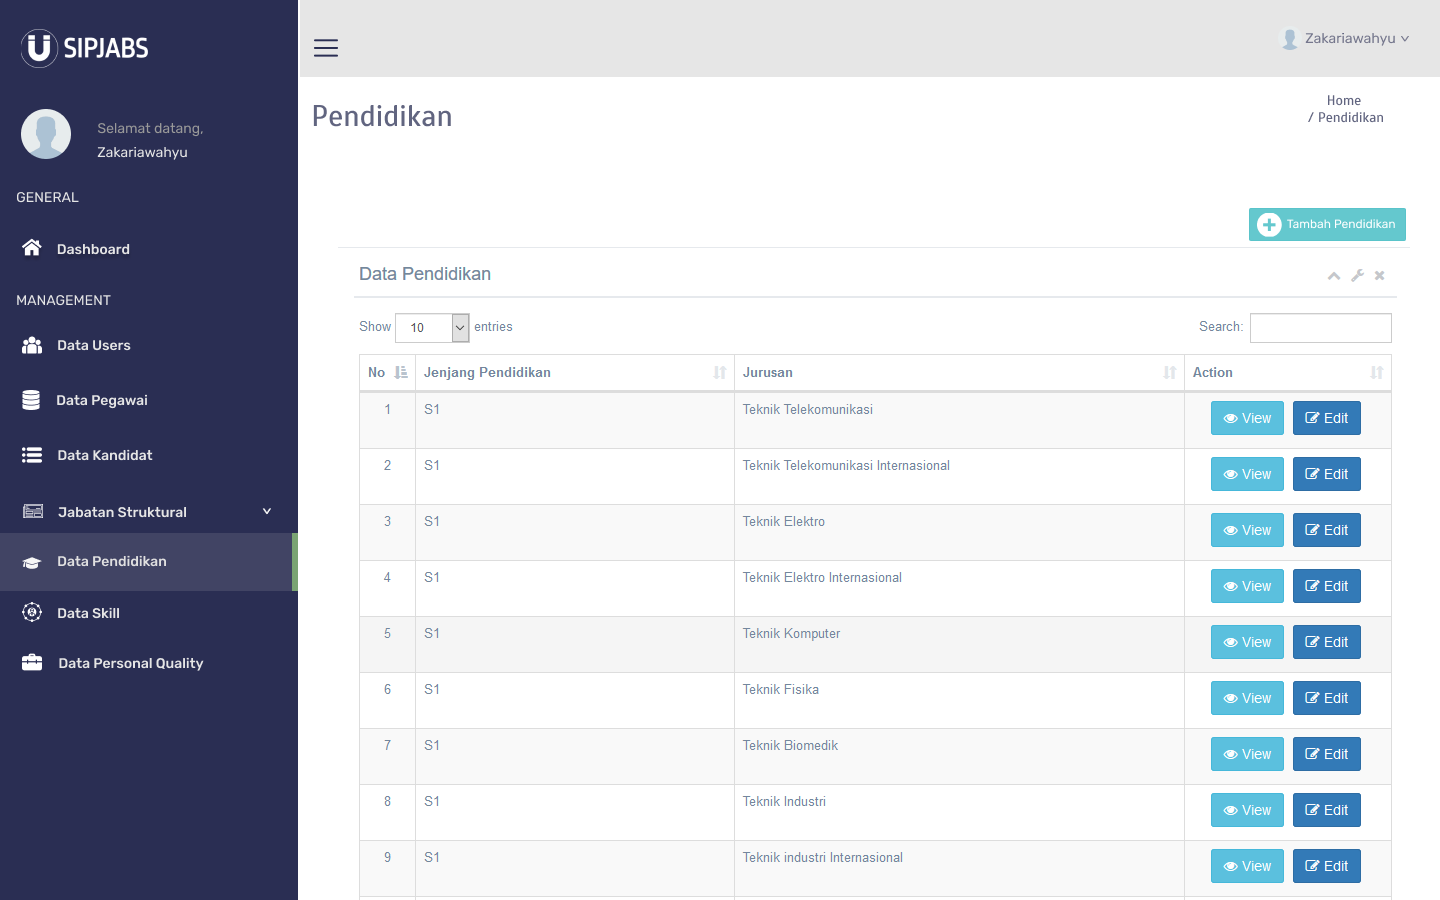
\includegraphics[width=0.6\textwidth, height=60mm]{pics/admin/datapendidikan.png}} 
		&Halaman ini akan menampilkan data pendidikan yang dimiliki pegawai Universitas Telkom.  \\
		
		\hline
		
		29. & \raisebox{-\totalheight}{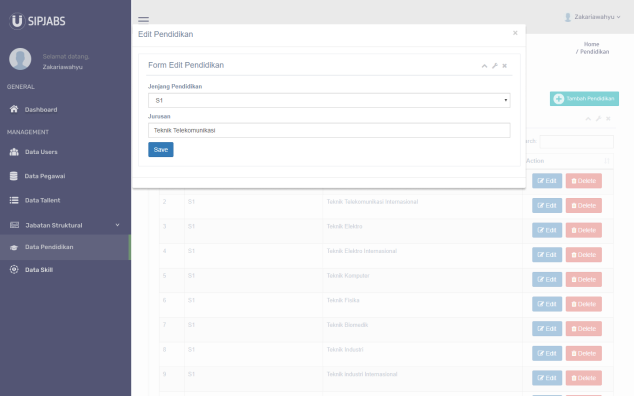
\includegraphics[width=0.6\textwidth, height=60mm]{pics/admin/editpendidikan.png}} 
		& Apabila ingin mengedit maka admin harus menginputkan jenjang pendidikan serta jurusan. \\
		
		\hline
		
	\end{tabular}
\end{table}

\begin{table}
	\caption{Tabel Perancangan Antar Muka Admin (10)}
	\centering
	\begin{tabular}{ | c | c | p{35mm} |}
		\hline 
		\textbf{No} & \textbf{Gambar} &  \textbf{Keterangan} \\ 
		\hline
		
		30. & \raisebox{-\totalheight}{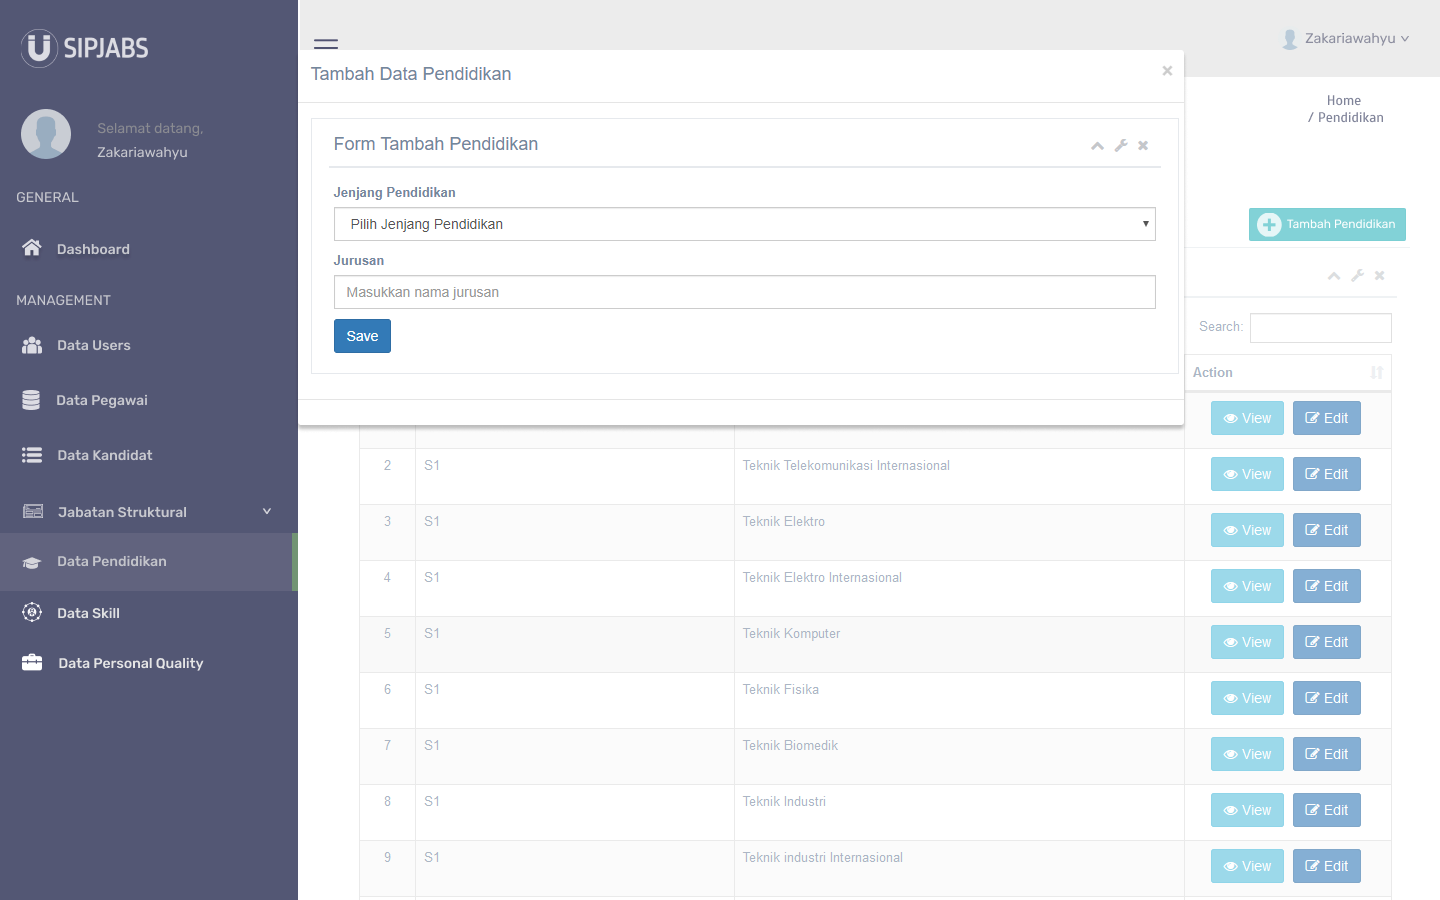
\includegraphics[width=0.6\textwidth, height=60mm]{pics/admin/tambahpendidikan.png}} 
		& Admin dapat menambahkan data pendidikan apabila belum ada data pendidikan yang dimiliki pegawai belum terinput. \\
		
		\hline
		
		31. & \raisebox{-\totalheight}{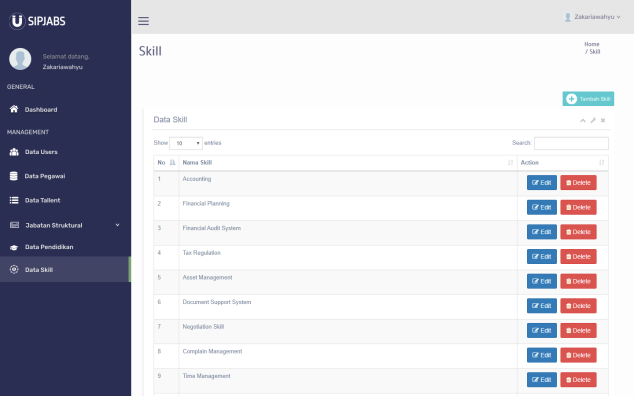
\includegraphics[width=0.6\textwidth, height=60mm]{pics/admin/dataskill.png}} 
		&Halaman ini akan menampilkan skill yang dimiliki pegawai Universitas Telkom untuk menunjang pekerjaan.  \\
		
		\hline
		
		32. & \raisebox{-\totalheight}{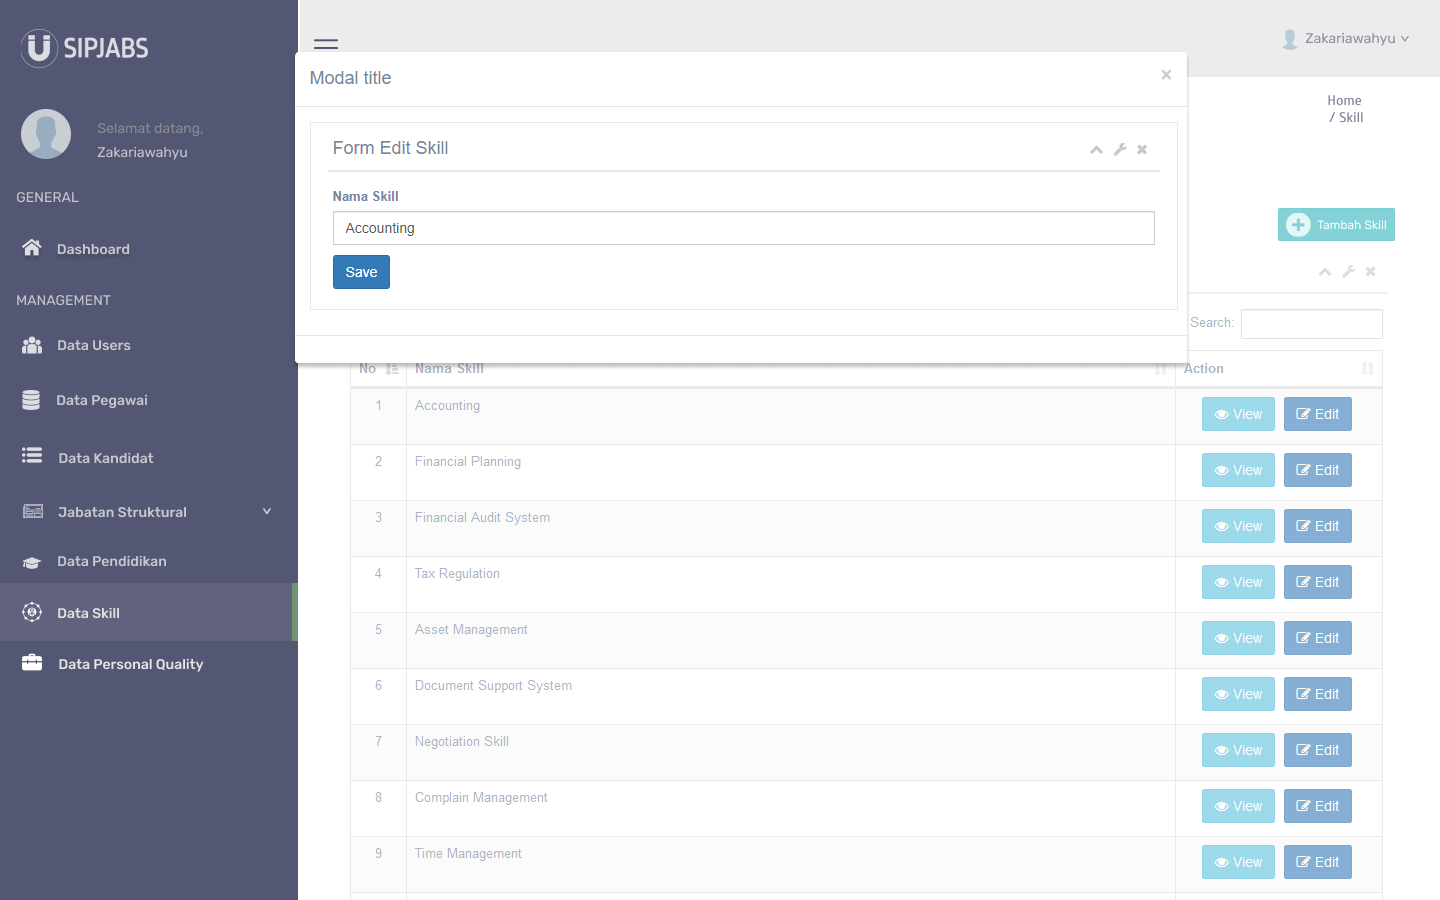
\includegraphics[width=0.6\textwidth, height=60mm]{pics/admin/editskill.png}} 
		& Admin dapat mengedit data skill. \\
		
		\hline
		
	\end{tabular}
\end{table}

\begin{table}
	\caption{Tabel Perancangan Antar Muka Admin (11)}
	\centering
	\begin{tabular}{ | c | c | p{35mm} |}
		\hline 
		\textbf{No} & \textbf{Gambar} &  \textbf{Keterangan} \\ 
		\hline
		
		33. & \raisebox{-\totalheight}{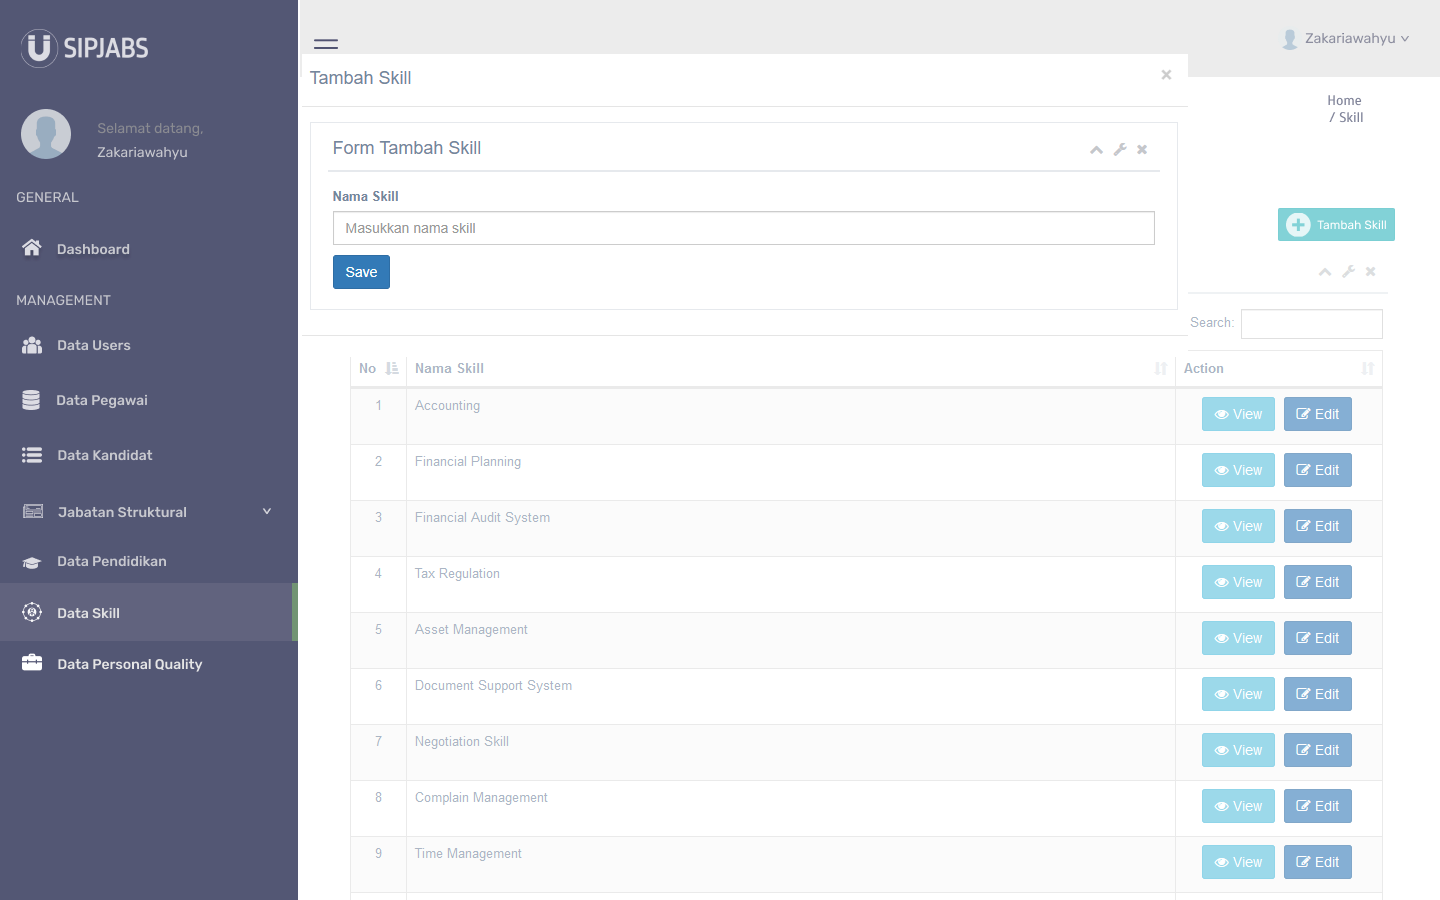
\includegraphics[width=0.6\textwidth, height=60mm]{pics/admin/tambahskill.png}} 
		& Admin dapat menambahkan data skill baru apabila terdapat data skill yang belum diinputkan.  \\
		
		\hline

		
	\end{tabular}
\end{table}

\subsubsection{Perancangan Antar Muka User}

\begin{table}
	\caption{Tabel Perancangan Antar Muka User}
	\centering
	\begin{tabular}{ | c | c | p{35mm} |}
		\hline 
		\textbf{No} & \textbf{Gambar} &  \textbf{Keterangan} \\ 
		\hline
		
		1. & \raisebox{-\totalheight}{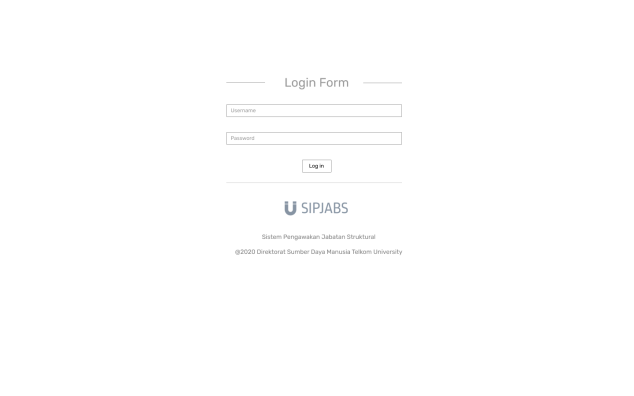
\includegraphics[width=0.6\textwidth, height=60mm]{pics/user/login.png}} 
		& Halaman login merupakan tampilan awal apabila user membuka aplikasi SiPJabS ,user dapat menginputkan username dan password untuk melakukan login.  \\
		
		\hline
		
		2. & \raisebox{-\totalheight}{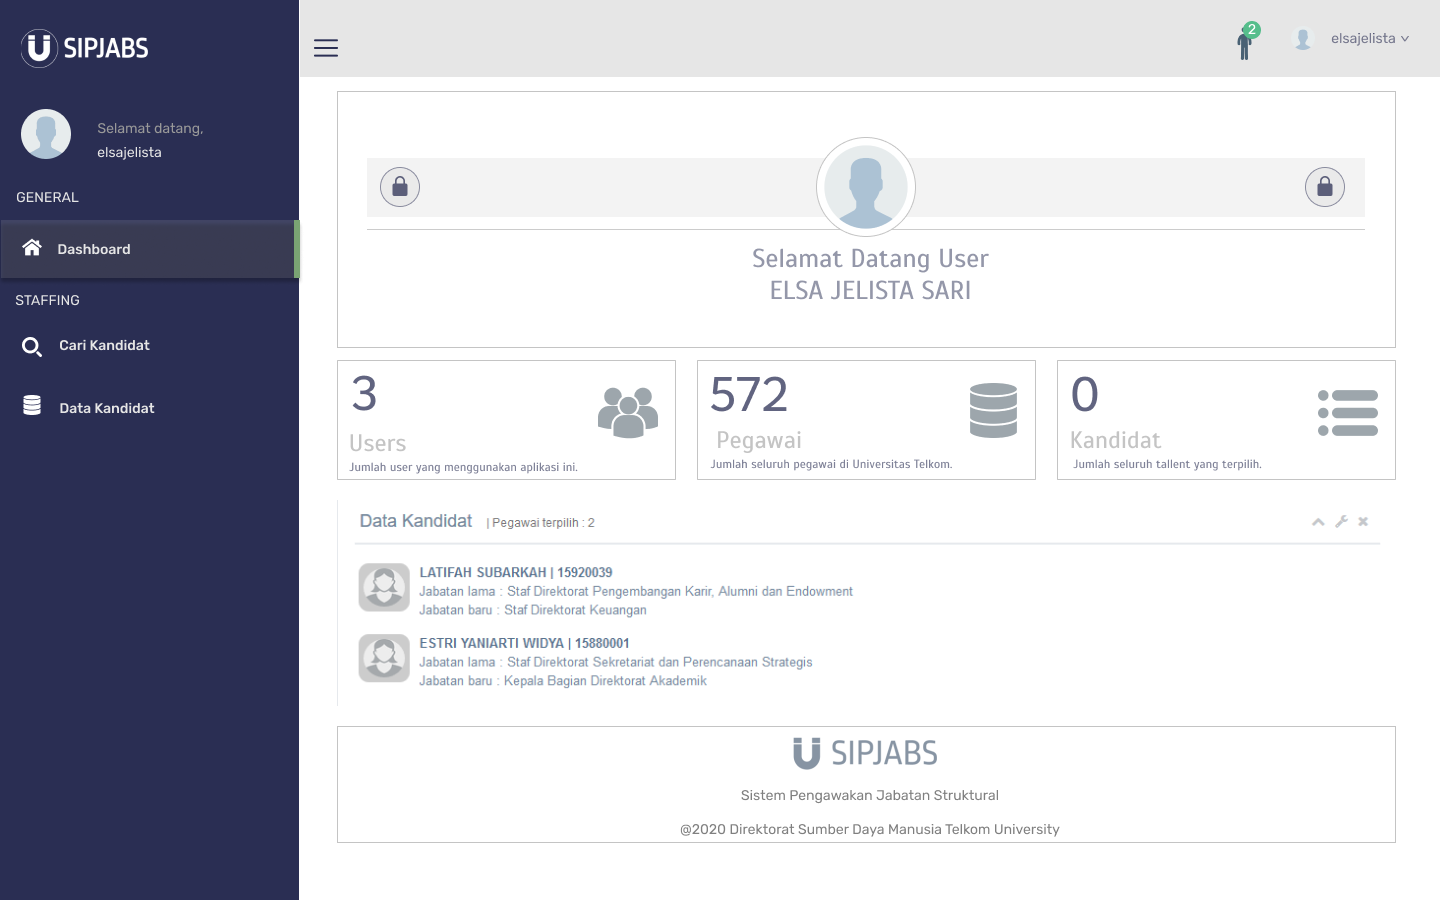
\includegraphics[width=0.6\textwidth, height=60mm]{pics/user/dashboard.png}} 
		& Halaman ini akan menampilkan jumlah user yang dapat mengakses aplikasi SiPJabS, jumlah pegawai yang ada di Universitas Telkom serta jumlah tallent yang sudah dipilih.  \\
		
		\hline
		
		3. & \raisebox{-\totalheight}{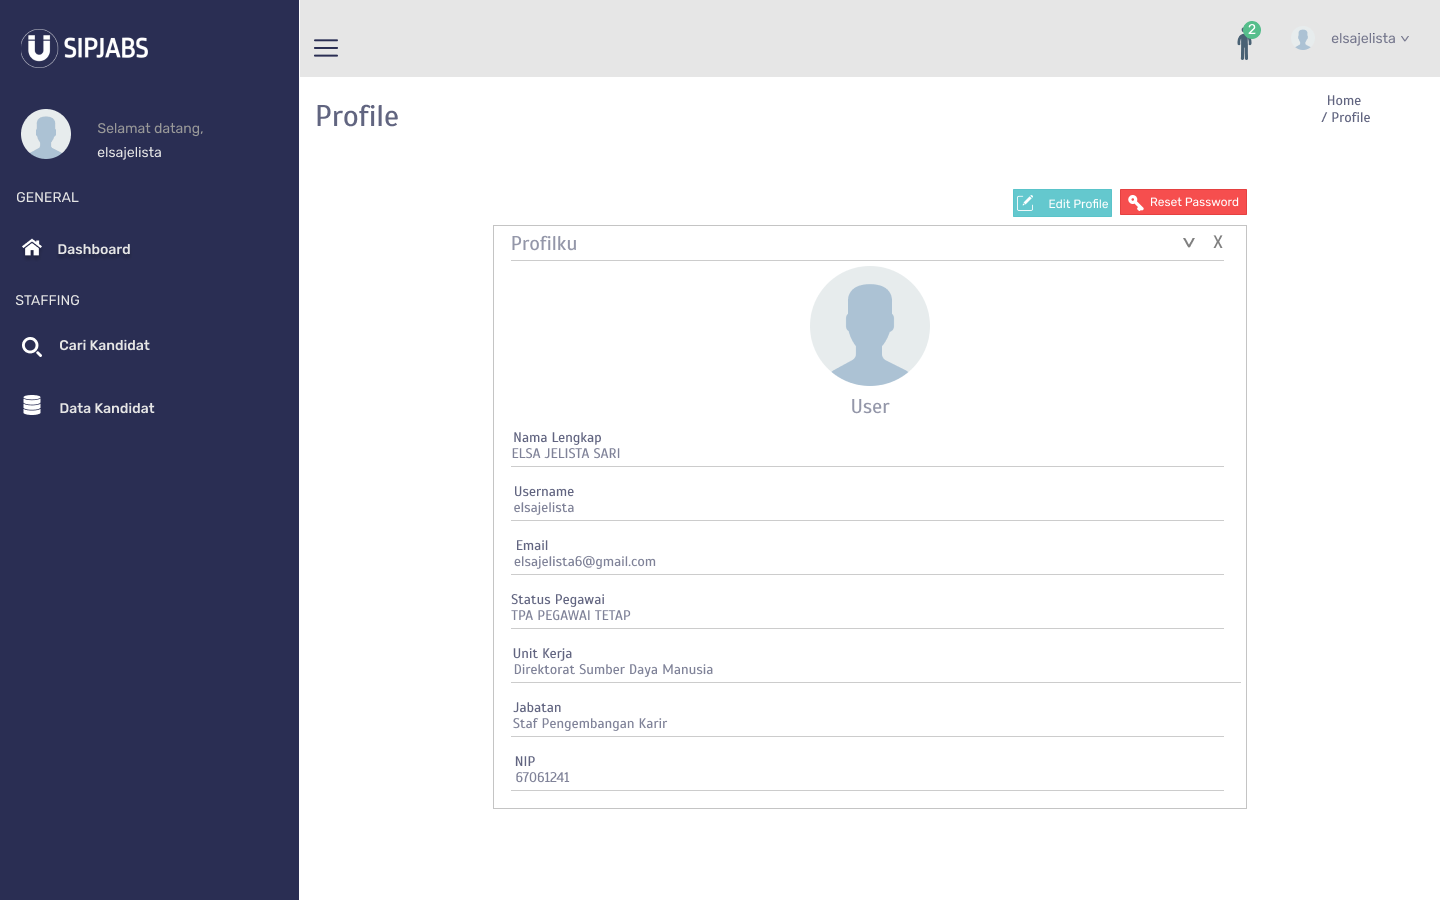
\includegraphics[width=0.6\textwidth, height=60mm]{pics/user/profile.png}} 
		& Halaman profile user akan menampilkan data nama lengkap, username, email, status pegawai, unit kerja, jabatan, serta NIP dari user tersebut. Kemudian user juga dapat mengedit profile dan mereset password.\\
		
		\hline
		
		
	\end{tabular}
\end{table}

\begin{table}
	\caption{Tabel Perancangan Antar Muka User (1)}
	\centering
	\begin{tabular}{ | c | c | p{35mm} |}
		\hline 
		\textbf{No} & \textbf{Gambar} &  \textbf{Keterangan} \\ 
		\hline
		
		4. & \raisebox{-\totalheight}{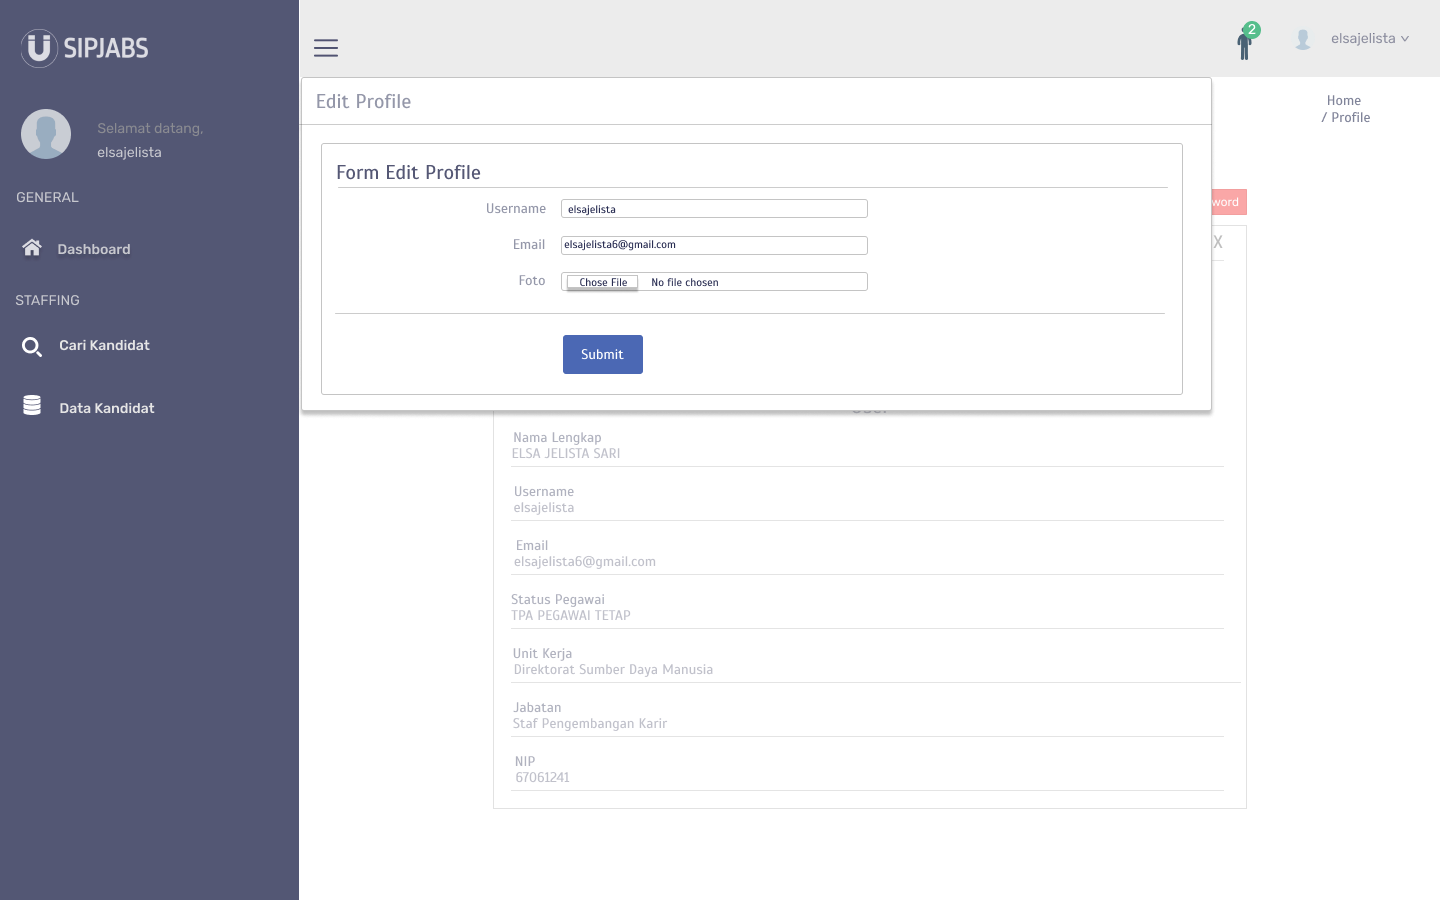
\includegraphics[width=0.6\textwidth, height=60mm]{pics/user/editprofile.png}} 
		& User dapat mengubah username, menginputkan email, dan menambahkan foto profile  \\
		
		\hline
		
		5. & \raisebox{-\totalheight}{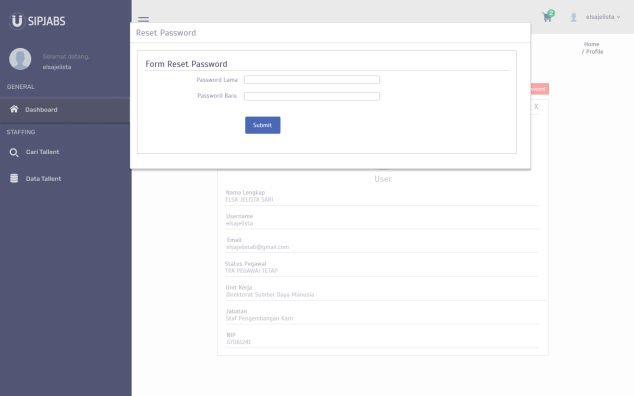
\includegraphics[width=0.6\textwidth, height=60mm]{pics/user/resetpassword.png}} 
		& User harus menginputkan password yang lama serta yang baru, setelah itu user dapat menyimpan.  \\
		
		\hline
		
		6. & \raisebox{-\totalheight}{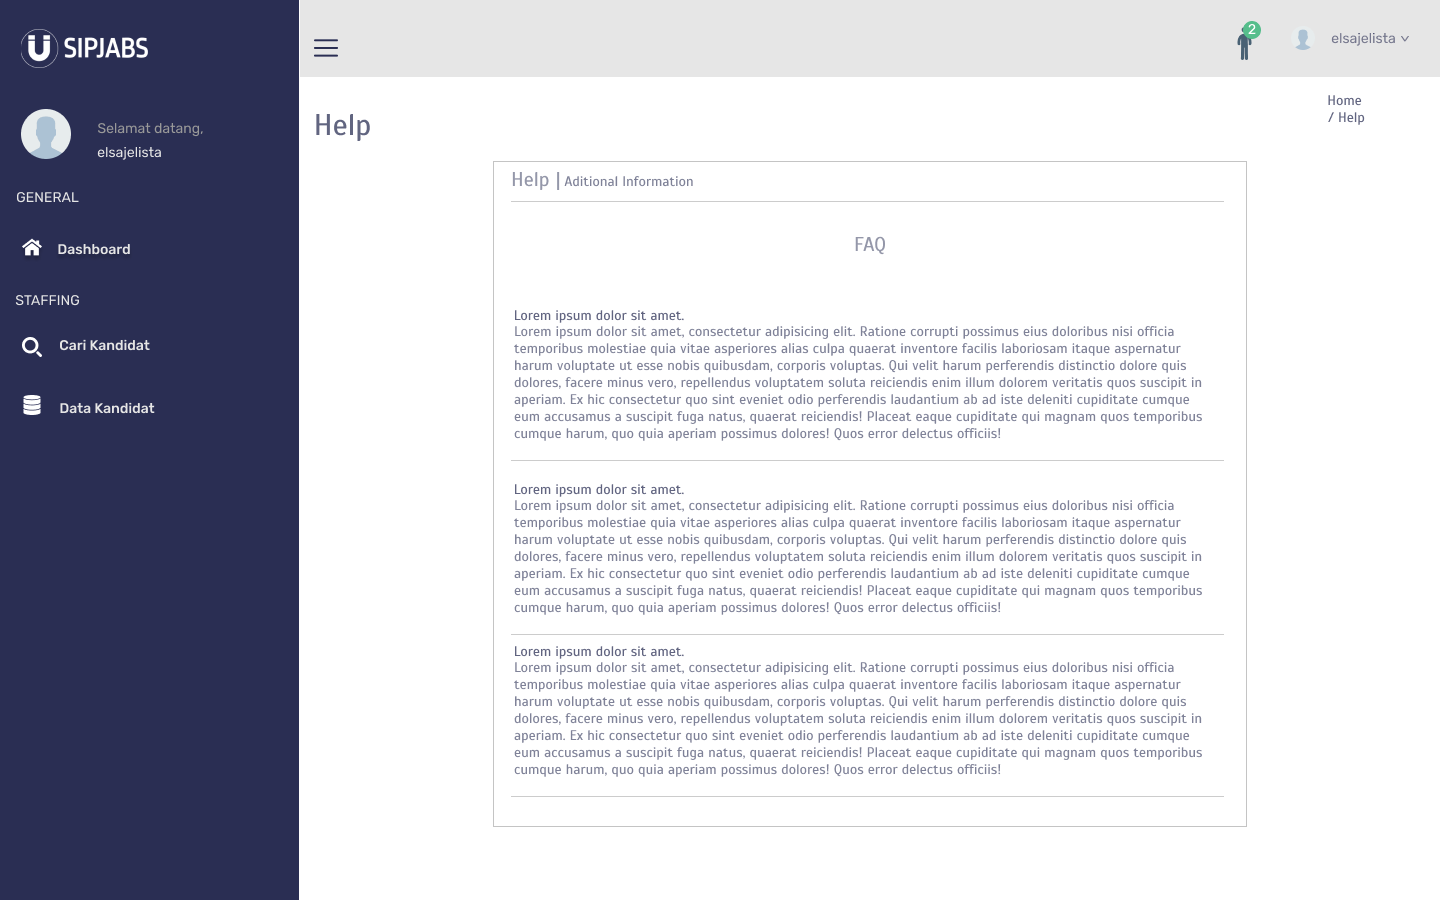
\includegraphics[width=0.6\textwidth, height=60mm]{pics/user/help.png}} 
		& Pada halaman help akan mengenai informasi dari sistem aplikasi ini\\
		
		\hline
		
	\end{tabular}
\end{table}

\begin{table}
	\caption{Tabel Perancangan Antar Muka User (1)}
	\centering
	\begin{tabular}{ | c | c | p{35mm} |}
		\hline 
		\textbf{No} & \textbf{Gambar} &  \textbf{Keterangan} \\ 
		\hline
		
		7. & \raisebox{-\totalheight}{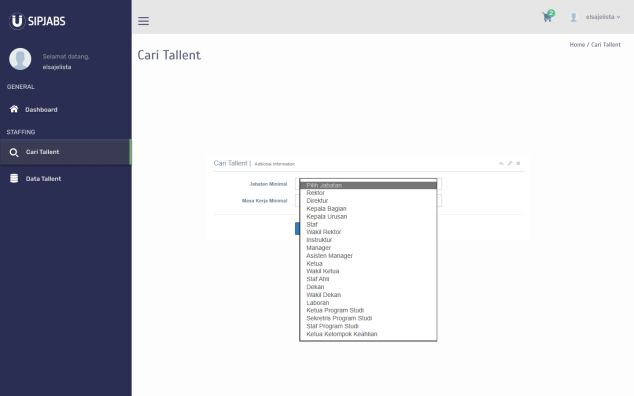
\includegraphics[width=0.6\textwidth, height=60mm]{pics/user/caritallent.png}} 
		& User dapat memilih jabatan dan masa kerja yang diinginkan untuk mengantikan atau mengisi posisi yang kosong.  \\
		
		\hline
		
		8. & \raisebox{-\totalheight}{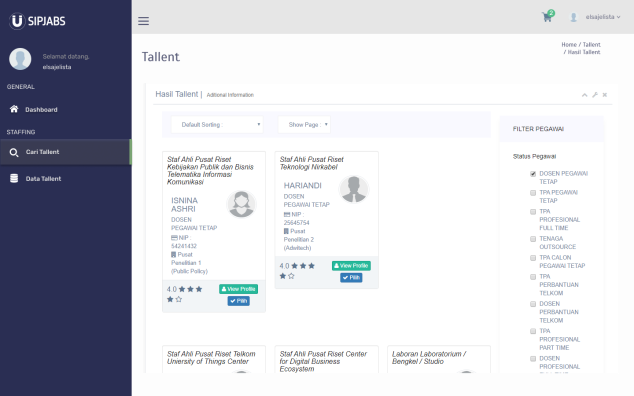
\includegraphics[width=0.6\textwidth, height=60mm]{pics/user/hasiltallent.png}} 
		& Halaman ini akan menampilkan tallent yang sudah di pilih dengan syarat tententu.   \\
		
		\hline
		
		9. & \raisebox{-\totalheight}{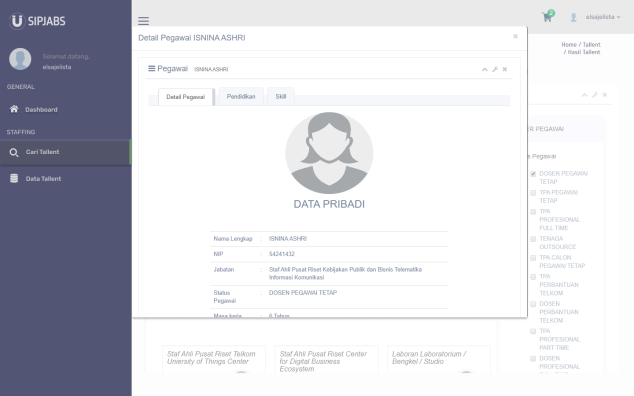
\includegraphics[width=0.6\textwidth, height=60mm]{pics/user/viewdetailtallent.png}} 
		& Halaman ini akan menampilkan data pribadi dari tallent tersebut.\\
		
		\hline
		
	\end{tabular}
\end{table}

\begin{table}
	\caption{Tabel Perancangan Antar Muka User (1)}
	\centering
	\begin{tabular}{ | c | c | p{35mm} |}
		\hline 
		\textbf{No} & \textbf{Gambar} &  \textbf{Keterangan} \\ 
		\hline
		
		10. & \raisebox{-\totalheight}{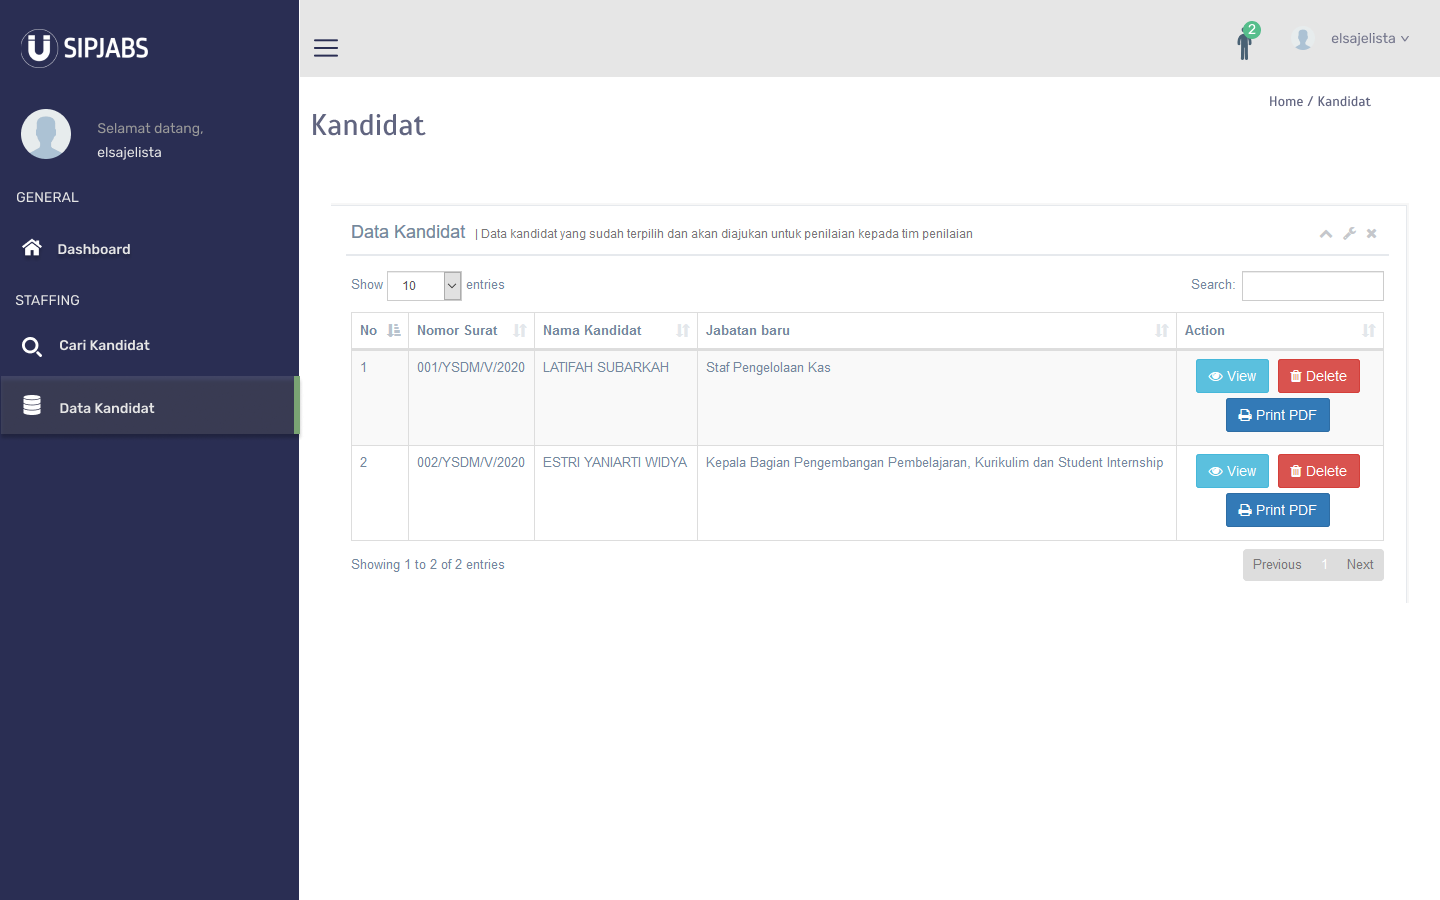
\includegraphics[width=0.6\textwidth, height=60mm]{pics/user/datatallent.png}} 
		& Halaman ini akan menampilkan data tallent yang sudah di proses dari cart tersebut.  \\
		
	
		\hline
		
	\end{tabular}
\end{table}
\subsection{Perancangan Level Tinggi}

\begin{figure}
	\centering
	\includegraphics[width=0.9\textwidth]
	{pics/highleveldesign.png}
	\caption{High Level Design}
	\label{fig:34}
\end{figure}

Alur perancanaan level tinggi pada aplikasi pengawakan pegawai dimulai dari pengambilan API dalam bentuk JSON Request ke server. Pengambilan data akan di filter berdasarkan dengan query yang dibuat berdasarkan data yang diperoleh dari database yang ada. Kemudian database akan memberikan umpan balik berupa JSON Response berdasarkan request data yang akan ditampilkan kepada pengguna. 



% Bab 4 : Pengujian
%-----------------------------------------------------------------------------%
\chapter{\babEmpat}
%-----------------------------------------------------------------------------%

%-----------------------------------------------------------------------------%
\section{Implementasi Aplikasi}
%-----------------------------------------------------------------------------%

Implementasi aplikasi merupakan tahapan realisasi dari perancangan yang telah dibuat. Pada tahap ini akan dilakukan penjelasan mengenai antarmuka aplikasi “\textbf{SiPJabS: Sistem Pengawakan Jabatan Struktural di Universitas Telkom}”. 

\subsection{Implementasi Antarmuka Aplikasi}
Antarmuka merupakan tampilan yang telah diimplmentasikan dari rancangan yang telah dibuat. Berikut merupakan hasil implementasi antarmuka aplikasi yang telah dibuat:

\subsubsection{Implementasi Admin}

\begin{enumerate}
	
	\item Halaman \textit{Login}
	\begin{figure}
		\centering
		\includegraphics[width=0.8\textwidth]
		{pics/admin/implementasi/login.png}
		\caption{Halaman \textit{Login} Admin}
		\label{fig:CC10}
	\end{figure}

	Gambar tampilan diatas merupakan implementasi dari BAB III dimana admin harus menginputkan \textit{username} dan \textit{password} untuk dapat melanjutkan penggunaan aplikasi, apabila sudah diinput lanjut untuk mengklik \textit{button “login”}. 
	
	\newpage
	\item Halaman \textit{Dashboard}
	\begin{figure}
		\centering
		\includegraphics[width=0.8\textwidth]
		{pics/admin/implementasi/dashboard.png}
		\caption{Halaman \textit{Dashboard} Admin}
		\label{fig:CC10}
	\end{figure}
	Gambar diatas menjelaskan isi dari \textit{dashboard} admin, dibagi menjadi beberapa bagian diantaranya: terdapat jumlah \textit{user} yang dapat mengakses aplikasi SiPJabS sebagai admin maupun \textit{user}. Apabia admin menambahkan atau menghapus \textit{user} maka jumlah tersebut dapat berubah. Terdapat jumlah pegawai di Universitas Telkom. Kemudian jumlah kandidat yang sudah dipilih oleh user untuk menggantikan atau mengisi posisi yang kosong. Dibawahnya terdapat unit kerja yang didalamnya terdapat beberapa jabatan, dan didalam unit kerja juga dibagi menjadi unit bagian, agar pekerjaan lebih mudah untuk dikerjakan. Kemudian terdapat pendidikan yang dimiliki oleh pegawai Universitas Telkom, dan terakhir terdapat \textit{skill} yang dimiliki pegawai Universitas Telkom guna menunjang kerja.
	
	\newpage
	\item Halaman \textit{Profile}
	\begin{figure}
		\centering
		\includegraphics[width=0.8\textwidth]
		{pics/admin/implementasi/profile.png}
		\caption{Halaman \textit{Profile} Admin}
		\label{fig:CC10}
	\end{figure}
	Implementasi diatas menjelaskan bahwasannya admin dapat melihat \textit{profile} dengan mengklik \textit{username} yang berada di atas kanan, kemudian akan terdapat \textit{dropdown}, lalu klik \textit{profile}, maka akan tampil \textit{profile} dari admin.
	
	\item Halaman \textit{Edit Profile}
	\begin{figure}
		\centering
		\includegraphics[width=0.8\textwidth]
		{pics/admin/implementasi/editprofile.png}
		\caption{Halaman \textit{Edit Profile} Admin}
		\label{fig:CC10}
	\end{figure}
	Gambar diatas mengimplementasikan bahwasannya admin dapat mengedit data \textit{profile} dengan mengklik \textit{button “edit profile”} kemudian dapat mengganti \textit{username} atau email dan foto. Lalu admin harus mengklik “\textit{submit}” untuk dapat menyimpan data yang sudah diperbarui. 
	
	\newpage
	\item Halaman \textit{Reset Password}
	\begin{figure}
		\centering
		\includegraphics[width=0.8\textwidth]
		{pics/admin/implementasi/resetpassword.png}
		\caption{Halaman \textit{Reset Password} Admin}
		\label{fig:CC10}
	\end{figure}
	Implementasi diatas menandakan bahwasannya admin dapat mengganti \textit{password} apabila \textit{password} terebut sudah diketahui oleh pihak lain, dengan klik \textit{button “reset password”} kemudian akan tampil halaman \textit{pop-up} seperti diatas, admin cukup menginputkan \textit{password} lama dan \textit{password} baru, lalu klik “\textit{submit}” untuk menyimpan \textit{password} yang sudah diganti. 
	
	\item Halaman \textit{Help}
	\begin{figure}
		\centering
		\includegraphics[width=0.8\textwidth]
		{pics/admin/implementasi/help.png}
		\caption{Halaman \textit{Help} Admin}
		\label{fig:CC10}
	\end{figure}

	\newpage
	\item Halaman Data \textit{Users}
	\begin{figure}
		\centering
		\includegraphics[width=0.8\textwidth]
		{pics/admin/implementasi/datausers.png}
		\caption{Halaman Data \textit{Users} - Admin}
		\label{fig:CC10}
	\end{figure}
	Gambar diatas menjelaskan isi dari halaman data \textit{users}, dimana admin dapat mengelola \textit{users} yang bisa mengakses aplikasi \textbf{SiPJabS}, karena apikasi ini hanya dapat diakses oleh orang-orang tententu. 
	
	\item Halaman \textit{Edit} Data \textit{Users}
	\begin{figure}
		\centering
		\includegraphics[width=0.8\textwidth]
		{pics/admin/implementasi/editusers.png}
		\caption{Halaman \textit{Edit} Data \textit{Users} - Admin}
		\label{fig:CC10}
	\end{figure}
	Gambar diatas menjelaskan bahwasannya data \textit{users} dapat diedit seperti \textit{username}, email, dan \textit{role} yang digunakan sebagai admin atau \textit{user}. Apabila data sudah diubah admin dapat mengklik \textit{button “Submit”} untuk menyelesaikan proses.
	
	\newpage
	\item Halaman Tambah \textit{Users}
	\begin{figure}
		\centering
		\includegraphics[width=0.8\textwidth]
		{pics/admin/implementasi/tambahusers.png}
		\caption{Halaman Tambah \textit{Users} - Admin}
		\label{fig:CC10}
	\end{figure}
	Dari tampilan diatas dapat dijelaskan, hanya admin saja yang dapat menambahkan data \textit{user}, namun harus sesuai dengan perintah dan \textit{job description} pegawai. Dengan mencari nama pegawai, menginputkan \textit{username}, \textit{password}, email, dan \textit{role}nya sebagai admin atau \textit{user}. Untuk mengakhiri proses admin dapat menyimpan apabila sudah disimpan akan terdapat \textit{pop-up}.
	
	\item Halaman Data Pegawai
	\begin{figure}
		\centering
		\includegraphics[width=0.8\textwidth]
		{pics/admin/implementasi/datapegawai.png}
		\caption{Halaman Data Pegawai - Admin}
		\label{fig:CC10}
	\end{figure}
	Dari tampilan diatas dijelaskan bahwasannya admin dapat melihat data seluruh pegawai yang ada di Universitas Telkom dengan mengklik menu “Data Pegawai” yang ada di sebelah kiri.
	
	\item Halaman \textit{View Detail} Pegawai
	\begin{figure}
		\centering
		\includegraphics[width=0.8\textwidth]
		{pics/admin/implementasi/viewdetailpegawai.png}
		\caption{Halaman \textit{View Detail} Pegawai - Admin}
		\label{fig:CC10}
	\end{figure}
	Untuk implementasi \textit{view detail} pegawai admin dapat mengklik \textit{button view}, maka akan tampil seperti gambar diatas. Terdapat data pribadi dari pegawai yang dapat dilihat diantaranya: nama lengkap, NIP, jabatan, status pegawai, masa kerja, tempat lahir, tanggal lahir, status perkawinan, golongan darah, jenis kelamin, agama, tinggi badan, berat badan, dan alamat.
	
	\item Halaman \textit{Edit} Pegawai
	\begin{figure}
		\centering
		\includegraphics[width=0.8\textwidth]
		{pics/admin/implementasi/editpegawai.png}
		\caption{Halaman \textit{Edit} Pegawai - Admin}
		\label{fig:CC10}
	\end{figure}
	Untuk implementasi \textit{edit} pegawai admin dapat mengklik \textit{button} edit, maka akan tampil seperti gambar diatas dan dapat mengedit data yang ada.
	
	\newpage
		\item Halaman Data Kandidat
	\begin{figure}
		\centering
		\includegraphics[width=0.8\textwidth]
		{pics/admin/implementasi/datatallent.png}
		\caption{Halaman Data Kandidat - Admin}
		\label{fig:CC10}
	\end{figure}
	Gambar diatas menampilkan halaman data kandidat yang dapat dilihat apabila admin mengklik menu “Data Kandidat”. Terdapat data kandidat yang sudah dipilih oleh \textit{user}, sesuai dengan \textit{requirement} yang telah ditetapkan perusahaan guna mengganti atau mengisi posisi yang kosong.  
	
	\item Halaman \textit{View Detail} Kandidat
	\begin{figure}
		\centering
		\includegraphics[width=0.8\textwidth]
		{pics/admin/implementasi/viewdetailtallent.png}
		\caption{Halaman \textit{View Detail} Kandidat - Admin}
		\label{fig:CC10}
	\end{figure}
	Tampilan diatas akan muncul apabila admin mengklik \textit{button “view”}. Kemudian tampil \textit{detail} data pegawai yang suda dipilih oleh \textit{user}, seperti data pribadi, jenjang pendidikan, dan \textit{skill}. 
	
	\newpage
	\item Halaman Data Unit Kerja
	\begin{figure}
		\centering
		\includegraphics[width=0.8\textwidth]
		{pics/admin/implementasi/dataunitkerja.png}
		\caption{Halaman Data Unit Kerja - Admin}
		\label{fig:CC10}
	\end{figure}
	Untuk implementasi diatas admin harus klik “jabatan struktural” kemudian akan terdapat \textit{dropdown}, lalu klik “data unit kerja” maka akan menampilkan data unit kerja yang berada di Universitas Telkom dari rektorat hingga ke fakultas. 
	
	\item Halaman \textit{Edit} Unit Kerja
	\begin{figure}
		\centering
		\includegraphics[width=0.8\textwidth]
		{pics/admin/implementasi/editunitkerja.png}
		\caption{Halaman \textit{Edit} Unit Kerja - Admin}
		\label{fig:CC10}
	\end{figure}
	Gambar diatas akan muncul apabila admin mengklik \textit{button “edit”} kemudian akan tampil \textit{pop-up} edit unit kerja, apabila nama unit kerja mengalami perubahan yang sudah ditetapkan. 
	
	\newpage
	\item Halaman Tambah Unit Kerja
	\begin{figure}
		\centering
		\includegraphics[width=0.8\textwidth]
		{pics/admin/implementasi/tambahunitkerja.png}
		\caption{Halaman Tambah Unit Kerja - Admin}
		\label{fig:CC10}
	\end{figure}
	Implementasi diatas akan muncul apabila admin mengklik \textit{button} “tambah unit kerja”, apabila terdapat unit kerja baru yang sudah ditetapkan, maka admin dapat menambahkannya. Untuk menyelesaikan proses admin harus mengklik \textit{button “save”}, kemudian data akan tersimpan.
	
	\item Halaman Data Jabatan
	\begin{figure}
		\centering
		\includegraphics[width=0.8\textwidth]
		{pics/admin/implementasi/datajabatan.png}
		\caption{Halaman Data Jabatan - Admin}
		\label{fig:CC10}
	\end{figure}
	Gambar diatas menampilkan data jabatan apabila admin mengklik menu “data jabatan” pada \textit{dropdown} ”jabatan struktural”. Terdapat nama-nama jabatan yang ada di Universitas Telkom yang akan terhubung dengan unit kerja dan unit bagian.  
	
	\item Halaman \textit{Edit} Jabatan
	\begin{figure}
		\centering
		\includegraphics[width=0.8\textwidth]
		{pics/admin/implementasi/editjabatan.png}
		\caption{Halaman \textit{Edit} Jabatan - Admin}
		\label{fig:CC10}
	\end{figure}
	Untuk tampilan diatas adalah \textit{form edit} jabatan, admin dapat mengklik \textit{button “edit”} kemudian menginputkan nama jabatan serta level jabatan, dan menyimpannya untuk mengakhiri proses, kemudian data akan tersimpan.
	
	\item Halaman Tambah Jabatan
	\begin{figure}
		\centering
		\includegraphics[width=0.8\textwidth]
		{pics/admin/implementasi/tambahjabatan.png}
		\caption{Halaman Tambah Jabatan - Admin}
		\label{fig:CC10}
	\end{figure}
	Gambar diatas menampilkan \textit{pop-up form} tambah jabatan, tampilan tersebut akan muncul apabila admin mengklik \textit{button} “tambah jabatan”. Kemudian admin menginputkan nama jabatan dan level jabatan untuk membuat jabatan baru yang sudah ditetapkan. Lalu simpan data tersebut dengan mengklik \textit{button “save”} maka data akan tesimpan di jabatan.
	
	\item Halaman Data Unit Bagian
	\begin{figure}
		\centering
		\includegraphics[width=0.8\textwidth]
		{pics/admin/implementasi/dataunitbagian.png}
		\caption{Halaman Data Unit Bagian - Admin}
		\label{fig:CC10}
	\end{figure}
	Untuk tampilan diatas adalah tampilan dari data unit bagian, didapat apabila admin mengklik \textit{dropdown} “jabatan struktural” pada menu kemudian mengklik “data unit bagian”, halaman ini menjelaskan bagian dari unit kerja yang ada di Universitas Telkom. Diharapkan dapat menyelesaikan pekerjaan sesuai dengan unit bagian masing-masing secara efektif dan maksimal.
	
	\item Halaman \textit{Edit} Unit Bagian
	\begin{figure}
		\centering
		\includegraphics[width=0.8\textwidth]
		{pics/admin/implementasi/editunitbagian.png}
		\caption{Halaman \textit{Edit} Unit Bagian - Admin}
		\label{fig:CC10}
	\end{figure}
	Gambar diatas menampilkan \textit{form edit} unit bagian, didapat apabila admin mengklik \textit{button ”edit”} kemudian admin dapat menginputkan nama unit bagian yang baru dan sesuai dengan ketetapan, terakhir klik \textit{button “save”} sehingga data akan tersimpan kembali.
	
	\item Halaman Tambah Unit Bagian
	\begin{figure}
		\centering
		\includegraphics[width=0.8\textwidth]
		{pics/admin/implementasi/tambahunitbagian.png}
		\caption{Halaman Tambah Unit Bagian - Admin}
		\label{fig:CC10}
	\end{figure}
	Implementasi diatas menunjukkan bahwasannya admin dapat menambah data unit bagian dengan cara klik \textit{button} “tambah unit bagian” dan menginputkan nama unit bagian dan menyimpannya dengan mengklik \textit{button “save”}, kemudian data akan tersimpan didalam data unit bagian. 
	
	\item Halaman Data Jabatan Struktural
	\begin{figure}
		\centering
		\includegraphics[width=0.8\textwidth]
		{pics/admin/implementasi/datajabstruk.png}
		\caption{Halaman Data Jabatan Struktural - Admin}
		\label{fig:CC10}
	\end{figure}
	Untuk implementasi dari tampilan diatas admin dapat mengklik \textit{dropdown} “jabatan struktural” kemudian mengklik menu “data jabatan struktural”, makan akan tampil halaman jabatan struktural yang ada di Universitas Telkom. Terdiri dari unit kerja, jabatan, unit bagian serta formasi jabatan. 
	
	\item Halaman \textit{Edit} Jabatan Struktural
	\begin{figure}
		\centering
		\includegraphics[width=0.8\textwidth]
		{pics/admin/implementasi/editjabstruk.png}
		\caption{Halaman \textit{Edit} Jabatan Struktural - Admin}
		\label{fig:CC10}
	\end{figure}
	Gambar diatas mengimplementasikan \textit{pop-up} dari \textit{form edit} jabatan struktural, dimana admin harus menginputkan unit kerja, jabatan, unit bagian, dan formasi jabatan, lalu untuk mengakhiri proses admin harus mengklik \textit{button “save”} kemudian data yang diedit akan tersimpan. 
	
	\item Halaman Tambah Jabatan Struktural
	\begin{figure}
		\centering
		\includegraphics[width=0.8\textwidth]
		{pics/admin/implementasi/tambahjabstruk.png}
		\caption{Halaman Tambah Jabatan Struktural - Admin}
		\label{fig:CC10}
	\end{figure}
	Untuk tampilan diatas adalah \textit{form} tambah jabatan stuktural, didapat apabila admin mengklik \textit{button} “tambah jabatan struktural”, kemudian admin harus menginputkan data seperti unit kerja, jabatan, unit bagian, dan formasi jabatan, kemudian klik \textit{button “save”} untuk mengakhiri proses.
	
	\item Halaman Data Pendidikan
	\begin{figure}
		\centering
		\includegraphics[width=0.8\textwidth]
		{pics/admin/implementasi/datapendidikan.png}
		\caption{Halaman Data Pendidikan - Admin}
		\label{fig:CC10}
	\end{figure}
	Gambar diatas menjelaskan data pendidikan semua pegawai Universitas Tekom, sehingga admin dapat mengetahui bahwasannya pegawai di Universitas Telkom memiliki jenjang pendidikan dan jurusan apa saja. Didapat apabila admin megklik menu “data pendidikan”.
	
	\item Halaman \textit{Edit} Pendidikan
	\begin{figure}
		\centering
		\includegraphics[width=0.8\textwidth]
		{pics/admin/implementasi/editpendidikan.png}
		\caption{Halaman \textit{Edit} Pendidikan - Admin}
		\label{fig:CC10}
	\end{figure}
	Untuk tampilan diatas adalah tampilan \textit{pop-up} dari \textit{form edit} pendidikan, apabila admin ingin mengedit data pendidikan dengan mengklik \textit{button “edit”} kemudian memilih jenjang pendidikan dan menginputkan jurusan, apabila sudah sesuai klik \textit{button “save”} untuk menyimpan data.
	
	\item Halaman Tambah Pendidikan
	\begin{figure}
		\centering
		\includegraphics[width=0.8\textwidth]
		{pics/admin/implementasi/tambahpendidikan.png}
		\caption{Halaman Tambah Pendidikan - Admin}
		\label{fig:CC10}
	\end{figure}
	Gambar diatas menampilkan \textit{pop-up} tambah data pendidikan, apabila terdapat pegawai baru, namun data pendidikan belum terdaftar maka admin dapat menambahkannya dengan memilih jenjang pendidikan dan menginput jurusan,  kemudian diakhiri dengan mengklik \textit{button “save”} dan data akan tersimpan.
	
	\item Halaman Data \textit{Skill}
	\begin{figure}
		\centering
		\includegraphics[width=0.8\textwidth]
		{pics/admin/implementasi/dataskill.png}
		\caption{Halaman Data \textit{Skill} - Admin}
		\label{fig:CC10}
	\end{figure}
	Gambar diatas merupakan implementasi data \textit{skill} yang ada di Universitas Telkom, data tersebut ada karena setiap pegawai memiliki \textit{skill} kemudian data \textit{skill} dari semua pegawai disatukan didalam data \textit{skill},  untuk menunjang pekerjaan. 
	
	\item Halaman \textit{Edit Skill}
	\begin{figure}
		\centering
		\includegraphics[width=0.8\textwidth]
		{pics/admin/implementasi/editskill.png}
		\caption{Halaman \textit{Edit Skill} - Admin}
		\label{fig:CC10}
	\end{figure}
	Implementasi diatas menampikan \textit{pop-up form edit skill}, dimana admin dapat mengedit nama \textit{skill} menjadi lebih sesuai, dan menyimpannya kembali dengan mengklik \textit{button “save”}.
	
	\item Halaman Tambah Skill
	\begin{figure}
		\centering
		\includegraphics[width=0.8\textwidth]
		{pics/admin/implementasi/tambahskill.png}
		\caption{Halaman Tambah Skill - Admin}
		\label{fig:CC10}
	\end{figure}
	Untuk tampilan diatas adalah tambah data \textit{skill}, admin dapat menambahkan data \textit{skill} dengan mengkil button “tambah \textit{skill}” apabila \textit{skill} pada pegawai belum terdaftar pada data \textit{skill}, lalu inputkan nama \textit{skill} dan menyimpannya dengan klik \textit{button “save”}.
	
	\newpage
	\item Halaman Data \textit{Personal Quality}
	\begin{figure}
		\centering
		\includegraphics[width=0.8\textwidth]
		{pics/admin/implementasi/datapersonalquality.png}
		\caption{Halaman Data \textit{Personal Quality} - Admin}
		\label{fig:CC10}
	\end{figure}
	Gambar diatas merupakan implementasi data \textit{personal quality} yang ada di Universitas Telkom, data tersebut ada karena setiap pegawai memiliki \textit{personal quality} kemudian data \textit{skill} dari semua pegawai disatukan didalam data \textit{personal quality},  untuk menunjang pekerjaan. 
	
	\item Halaman \textit{Edit Personal Quality}
	\begin{figure}
		\centering
		\includegraphics[width=0.8\textwidth]
		{pics/admin/implementasi/editpersonalquality.png}
		\caption{Halaman \textit{Edit Personal Wuality} - Admin}
		\label{fig:CC10}
	\end{figure}
	Implementasi diatas menampikan \textit{pop-up form edit personal quality}, dimana admin dapat mengedit nama \textit{personal quality} menjadi lebih sesuai, dan menyimpannya kembali dengan mengklik \textit{button “save”}.
	
	\newpage
	\item Halaman Tambah Personal Quality
	\begin{figure}
		\centering
		\includegraphics[width=0.8\textwidth]
		{pics/admin/implementasi/tambahpersonalquality.png}
		\caption{Halaman Tambah Personal Quality - Admin}
		\label{fig:CC10}
	\end{figure}
	Untuk tampilan diatas adalah tambah data \textit{personal quality}, admin dapat menambahkan data \textit{personal quality} dengan mengkil button “tambah \textit{personal quality}”.
	
\end{enumerate}

\subsubsection{Implementasi \textit{User}}

\begin{enumerate}
	
	\item Halaman \textit{Login}
	\begin{figure}
		\centering
		\includegraphics[width=0.8\textwidth]
		{pics/user/implementasi/login.png}
		\caption{Halaman \textit{Login User}}
		\label{fig:CC10}
	\end{figure}
	
	Tampilan diatas merupakan implementasi dari BAB III dimana \textit{user} harus menginputkan \textit{username} dan \textit{password} untuk dapat melanjutkan penggunaan aplikasi, apabila sudah diinputkan lanjut untuk mengklik \textit{button “login”}. 
	
	\item Halaman \textit{Dashboard}
	\begin{figure}
		\centering
		\includegraphics[width=0.8\textwidth]
		{pics/user/implementasi/dashboard.png}
		\caption{Halaman \textit{Dashboard User}}
		\label{fig:CC10}
	\end{figure}
	
	Gambar diatas mengimplementasikan isi dari \textit{dashboard user}, berbeda dengan \textit{dashboard} yang dimiliki admin, \textit{dashboard user} hanya menampilkan jumlah \textit{user} yang dapat mengakses aplikasi \textbf{SiPJabS}, jumlah pegawai yang terdaftar di Universitas Telkom, serta jumlah kandidat yang sudah dipilih. 
	
	\item Halaman \textit{Profile}
	\begin{figure}
		\centering
		\includegraphics[width=0.8\textwidth]
		{pics/user/implementasi/profile.png}
		\caption{Halaman \textit{Profile User}}
		\label{fig:CC10}
	\end{figure}
	
	Implementasi diatas menunjukkan isi \textit{profile} dari \textit{user}, terdapat nama lengkap, \textit{username}, email, status pegawai, unit kerja, jabatan, dan NIP. Admin dapat membuka halaman tersebut dengan cara klik \textit{username} yang ada di atas kanan, kemudian akan terdapat \textit{dropdown} dan klik \textit{profile}, maka halaman akan tampil seperti diatas. 
	
	\item Halaman \textit{Edit Profile}
	\begin{figure}
		\centering
		\includegraphics[width=0.8\textwidth]
		{pics/user/implementasi/editprofile.png}
		\caption{Halaman \textit{Edit Profile User}}
		\label{fig:CC10}
	\end{figure}
	
	Gambar diatas mengimplementasikan\textit{ edit profile user} dengan \textit{pop-up}, \textit{user} dapat mengganti \textit{username}, email atau foto. Kemudian klik “\textit{submit}” untuk menyimpan data yang sudah diganti agar tersimpan.
	
	\item Halaman \textit{Reset Password}
	\begin{figure}
		\centering
		\includegraphics[width=0.8\textwidth]
		{pics/user/implementasi/resetpassword.png}
		\caption{Halaman \textit{Reset Password User}}
		\label{fig:CC10}
	\end{figure}
	
	Implementasi diatas menjelaskan bahwasannya \textit{user} dapat mengganti \textit{passsword}, apabila \textit{password} tersebut sudah diketahui oleh pihak lain, \textit{user} dapat mengklik \textit{button “reset password”} kemudian akan tampil\textit{ pop-up} seperti diatas, \textit{user} harus menginputkan \textit{password} lama dan \textit{password} yang baru, lalu klik “\textit{submit}” untuk menyimpan \textit{password} yang baru.
	
	\item Halaman \textit{Help}
	\begin{figure}
		\centering
		\includegraphics[width=0.8\textwidth]
		{pics/user/implementasi/help.png}
		\caption{Halaman \textit{Help User}}
		\label{fig:CC10}
	\end{figure}

	\item Halaman Cari Kandidat
	\begin{figure}
		\centering
		\includegraphics[width=0.8\textwidth]
		{pics/user/implementasi/caritallent.png}
		\caption{Halaman Cari Kandidat - User}
		\label{fig:CC10}
	\end{figure}
	
	Gambar diatas mengimplementasikan apabila \textit{user} ingin mencari kandidat yang dibutuhkan sesuai \textit{requirement} perusahaan untuk menggantikan atau mengisi posisi yang kosong, dengan cara klik “cari kandidat” pada menu, lalu akan muncul halaman seperti diatas, user harus memilih jabatan yang dituju, jabatan  minimal yang dibutuhkan dan menginputkan masa kerja. Dan klik \textit{button} “cari”.
	
	\newpage
	\item Halaman \textit{Filtering}
	\begin{figure}
		\centering
		\includegraphics[width=0.8\textwidth]
		{pics/user/implementasi/hasiltallent.png}
		\caption{Halaman \textit{Filtering - User}}
		\label{fig:CC10}
	\end{figure}
	
	Implementasi diatas menampilkan data kandidat yang tersedia, kemudian \textit{user} dapat menyeleksi kembali dengan memilih \textit{filter} pegawai, jenjang pendidikan, jurusan dan \textit{skill} yang dimiliki oleh pegawai.
	
	\item Halaman\textit{ View Detail} Pegawai
	\begin{figure}
		\centering
		\includegraphics[width=0.8\textwidth]
		{pics/user/implementasi/viewdetailpegawai.png}
		\caption{Halaman \textit{View Detail} Pegawai - \textit{User}}
		\label{fig:CC10}
	\end{figure}
	
	Gambar diatas mengimpementasikan bahwasannya \textit{user} dapat melihat data pribadi yang dimiliki kandidat, dengan cara klik\textit{ button “view”} maka akan tampil halaman seperti diatas dan menampilkan data pribadi pegawai beserta data riwayat pendidikan, skill dan personal quality.
	
	\newpage
	\item Halaman Kandidat Sementara
	\begin{figure}
		\centering
		\includegraphics[width=0.8\textwidth]
		{pics/user/implementasi/cartuser.png}
		\caption{Halaman \textit{Cart - User}}
		\label{fig:CC10}
	\end{figure}
	
	Gambar diatas menjelaskan bahwasannya \textit{user} sudah memilih kandidat yang sesuai dengan yang dibutuhkan untuk mengganti atau mengisi posisi yang kosong.  
	
	\item Halaman \textit{View} Kandidat Sementara
	\begin{figure}
		\centering
		\includegraphics[width=0.8\textwidth]
		{pics/user/implementasi/viewcart.png}
		\caption{Halaman \textit{View} Kandidat Sementara}
		\label{fig:CC10}
	\end{figure}
	
	Gambar diatas mengimplementasikan halaman \textit{view }pada kandidat sementara, apabila \textit{user} telah memilih kandidat maka data tersebut akan masuk kedalam kandidat sementara, sebelum diproses ke data kandidat. 
	
	\newpage
		\item Halaman Data Kandidat
	\begin{figure}
		\centering
		\includegraphics[width=0.8\textwidth]
		{pics/user/implementasi/datatallent.png}
		\caption{Halaman Data Kandidat}
		\label{fig:CC10}
	\end{figure}
	
	Gambar diatas mengimplementasikan isi dari  data kandidat yang dimiliki \textit{user}, data tersebut sudah dipilih sesuai dengan \textit{requirement} perusahaan dan sesuai dengan \textit{job descripton} yang dimiliki pegawai dan selanjutka anak diajukan untuk penilaian.
	
\end{enumerate}

\subsection{Struktur Kode}
Struktur kode merupakan kumpulan kode atau script yang berfungsi untuk menjalankan setiap perintah dalam setiap proses pembuatan aplikasi. Berikut struktur kode yang ada pada aplikasi SiPJabS:

\begin{table}
	\caption{Tabel Struktur Kode}
	\centering
	\begin{tabular}{ | l | l | p{20mm} | p{22mm} | p{47mm} |}
		\hline
		
		\textbf{No} & \textbf{Struktur Kode} & \textbf{Controller} & \textbf{Method} & \textbf{Deskripsi}  \\
		\hline
		
		
		\multirow{4}{*}{1} &  \multirow{4}{*}{User} & \multirow{4}{20mm}{} & index() &  \multirow{4}{47mm}{Berfungsi untuk melakukan proses menampilkan, menambah dan menghapus data kandidat sementara } \\
		& & Cart & show() & \\
		& & Controller & destroy() & \\
		& & & addCart() & \\
		\hline
		
		\multirow{5}{*}{2} &  \multirow{5}{*}{User} & \multirow{5}{20mm}{} & index() &  \multirow{5}{47mm}{Berfungsi untuk melakukan proses filtering pegawai untuk mencari kandidat berdasarkan requirement} \\
		& & Filter & show() & \\
		& & Controller & filterTallent() & \\
		& & & getJabatan() & \\
		& & & fetch() & \\
		\hline
		
		
	\end{tabular}
\end{table}

\newpage

\begin{table}
	\centering
		\caption{Tabel Struktur Kode (1)}
	\begin{tabular}{ | l | l | p{20mm} | p{22mm} | p{47mm} |}
		\hline
		
		\textbf{No} & \textbf{Struktur Kode} & \textbf{Controller} & \textbf{Method} & \textbf{Deskripsi}  \\
		\hline
		
		
		\multirow{5}{*}{3} &  \multirow{5}{*}{User} & \multirow{5}{20mm}{} & index() &  \multirow{5}{47mm}{Berfungsi untuk melakukan proses melihat profile akun, reset password dan edit profile pada user } \\
		& & Profile & show() & \\
		& & Controller & edit() & \\
		& & & update() & \\
		& & & resetPass() & \\
		\hline
		
		\multirow{5}{*}{4} &  \multirow{5}{*}{User} & \multirow{5}{20mm}{} & index() &  \multirow{5}{47mm}{Berfungsi untuk melakukan pengelolaan seperti menambahkan data kandidat terpilih, menghapus dan print pdf} \\
		& & Tallent & show() & \\
		& & Controller & destroy() & \\
		& & & cetak pdf() & \\
		& & & addTallent() & \\
		\hline
		
		5 & User & User Controller & index() & Berfungsi menampilkan halaman dashboard user \\
		\hline
		
		6 & Admin & Admin Controller & index() & Berfungsi menampilkan halaman dashboard admin \\
		\hline
		
		\multirow{6}{*}{7} &  \multirow{6}{*}{Admin} & \multirow{6}{20mm}{} & index() &  \multirow{6}{47mm}{Berfungsi untuk melakukan proses CRUD pada jabatan} \\
		& &  & create() & \\
		& & Jabatan & store() & \\
		& & Controller& show() & \\
		& & & edit() & \\
		& & & update() & \\
		\hline
		
		\multirow{6}{*}{8} &  \multirow{6}{*}{Admin} & \multirow{6}{20mm}{} & index() &  \multirow{6}{47mm}{Berfungsi untuk melakukan proses CRUD pada jabatan struktural} \\
		& & Jabatan  & create() & \\
		& & Struktural & store() & \\
		& & Controller& show() & \\
		& & & edit() & \\
		& & & update() & \\
		\hline
		
		\multirow{6}{*}{9} &  \multirow{6}{*}{Admin} & \multirow{6}{20mm}{} & index() &  \multirow{6}{47mm}{Berfungsi untuk melakukan proses CRUD pada pegawai} \\
		& &  & create() & \\
		& & Pegawai & store() & \\
		& & Controller& show() & \\
		& & & edit() & \\
		& & & update() & \\
		\hline
		
	\end{tabular}
\end{table}

\begin{table}
	\centering
	\caption{Tabel Struktur Kode (2)}
	\begin{tabular}{ | l | l | p{20mm} | p{22mm} | p{47mm} |}
		\hline
		
		\textbf{No} & \textbf{Struktur Kode} & \textbf{Controller} & \textbf{Method} & \textbf{Deskripsi}  \\
		\hline
		
		\multirow{6}{*}{10} &  \multirow{6}{*}{Admin} & \multirow{6}{20mm}{} & index() &  \multirow{6}{47mm}{Berfungsi untuk melakukan proses CRUD pada pendidikan} \\
		& &  & create() & \\
		& & Pendidikan & store() & \\
		& & Controller& show() & \\
		& & & edit() & \\
		& & & update() & \\
		\hline
		
		\multirow{6}{*}{11} &  \multirow{6}{*}{Admin} & \multirow{6}{20mm}{} & index() &  \multirow{6}{47mm}{Berfungsi untuk melakukan proses CRUD pada personal quality} \\
		& & Personal  & create() & \\
		& & Quality & store() & \\
		& & Controller& show() & \\
		& & & edit() & \\
		& & & update() & \\
		\hline
		
		\multirow{5}{*}{12} &  \multirow{5}{*}{Admin} & \multirow{5}{20mm}{} & index() &  \multirow{5}{47mm}{Berfungsi untuk melakukan proses melihat profile akun, reset password dan edit profile pada admin} \\
		& & Profile & show() & \\
		& & Controller& edit() & \\
		& & & update() & \\
		& & & resetPass() & \\
		\hline
		
		\multirow{4}{*}{13} &  \multirow{4}{*}{Admin} & \multirow{4}{20mm}{} & index() &  \multirow{4}{47mm}{Berfungsi untuk melakukan proses menampilkan, delete dan cetak pdf kandidat } \\
		& & Tallent& show() & \\
		& & Controller& destroy() & \\
		& & & cetak pdf() & \\
		\hline
		
	\end{tabular}
\end{table}

 
 


%-----------------------------------------------------------------------------%
\section{Pengujian Aplikasi}
%-----------------------------------------------------------------------------%
Pengujian aplikasi merupakan proses yang bertujuan untuk dapat menilai kesesuaian serta dapat menentukan kualitas dari aplikasi/sistem yang telah dibuat dengan cara menemukan bug dari aplikasi/sistem. Metode testing yang akan dilakukan adalah Pengujian Alpha dan Pengujian Beta.


%-----------------------------------------------------------------------------%
\subsection{Pengujian Alpha}
%-----------------------------------------------------------------------------%

Pengujian Aplha dilakukan sebelum aplikasi di distribusikan, salah satunya dilakukan pengujian dengan cara BlackBox. Pada pengujian blackbox untuk mengetahui fungsionalitas dan kesesuaian sistem berdasarkan rancangan yang telah dibuat.

\subsubsection{Pengujian Fungsionalitas}

\begin{table}
	\caption{Tabel Pengujian Login Admin}
	\centering
	\begin{tabular}{ | l | p{92mm} |}
		\hline
		
		Nomor Test & PF-O1  \\
		\hline
		
		Pengguna & Admin  \\
		\hline
		
		Judul & Login Admin  \\
		\hline
		
		\multirow{3}{*}{Teknik} & 
		1. Membuka website dengan mengunjungi link www.sipjabs.my.id dan akan muncul halaman login
		\raisebox{-\totalheight}{\includegraphics[width=0.65\textwidth, height=60mm]{pics/pengujian/pf1-1.png}}   \\
	
		
		& 2. Inputkan username : zakariawahyu dan password : admin pada form login berikut.
		\raisebox{-\totalheight}{\includegraphics[width=0.4\textwidth, height=60mm]{pics/pengujian/pf1-2.png}}  \\
	
		
		& 3. Klik button ‘Login’ untuk menyelesaikan proses login \\
		\hline
	
		Kriteria Keberhasilan & Sistem akan menampilkan halaman dashboard admin \\
		\hline
		
		Kondisi khusus & Username dan password sudah diberikan oleh admin \\
		\hline
		
		\multirow{2}{*}{Hasil} & Valid : Yes \\
		
		& Invalid : No \\
		\hline
		
		
	\end{tabular}
\end{table}

\begin{table}
	\caption{Tabel Pengujian Login User}
	\centering
	\begin{tabular}{ | l | p{92mm} |}
		\hline
		
		Nomor Test & PF-O2  \\
		\hline
		
		Pengguna & User  \\
		\hline
		
		Judul & Login User  \\
		\hline
		
		\multirow{3}{*}{Teknik} & 
		1. Membuka website dengan mengunjungi link www.sipjabs.my.id dan akan muncul halaman login
		\raisebox{-\totalheight}{\includegraphics[width=0.65\textwidth, height=60mm]{pics/pengujian/pf1-1.png}}   \\

		
		& 2. Inputkan username : elsajelista dan password : user pada form login berikut.
		\raisebox{-\totalheight}{\includegraphics[width=0.4\textwidth, height=60mm]{pics/pengujian/pf1-2.png}}  \\

		
		& 3. Klik button ‘Login’ untuk menyelesaikan proses login \\
		\hline
		
		Kriteria Keberhasilan & Sistem akan menampilkan halaman dashboard user \\
		\hline
		
		Kondisi khusus & Username dan password sudah diberikan oleh admin \\
		\hline
		
		\multirow{2}{*}{Hasil} & Valid : Yes \\

		
		& Invalid : No \\
		\hline
		
		
	\end{tabular}
\end{table}

\begin{table}
	\caption{Tabel Pengujian Cari Kandidat}
	\centering
	\begin{tabular}{ | l | p{92mm} |}
		\hline
		
		Nomor Test & PF-03  \\
		\hline
		
		Pengguna & User  \\
		\hline
		
		Judul & Cari Kandidat  \\
		\hline
		
		\multirow{3}{*}{Teknik} & 
		1.	Klik “Cari Kandidat” pada menu yang ada di sebelah kiri
		\raisebox{-\totalheight}{\includegraphics[width=0.3\textwidth, height=10mm]{pics/pengujian/pf3-1.png}}   \\
		
		
		& 2. Inputkan persyaratan umum seperti jabatan yang akan di tuju atau posisi target, kemudian dengan minimal jabatan dan kerja minimal.
		\raisebox{-\totalheight}{\includegraphics[width=0.6\textwidth, height=50mm]{pics/pengujian/pf3-2.png}}  \\
		
		
		& 3. Klik button ‘Cari’ untuk melakukan proses pencarian \\
		\hline
		
		Kriteria Keberhasilan & Sistem akan menampilkan nama-nama kandidat \\
		\hline
		
		Kondisi khusus & - \\
		\hline
		
		\multirow{2}{*}{Hasil} & Valid : Yes \\
		
		
		& Invalid : No \\
		\hline
		
		
	\end{tabular}
\end{table}

\begin{table}
	\caption{Tabel Pengujian Filtering}
	\centering
	\begin{tabular}{ | l | p{92mm} |}
		\hline
		
		Nomor Test & PF-04  \\
		\hline
		
		Pengguna & User  \\
		\hline
		
		Judul & Melakukan Filtering  \\
		\hline
		
		\multirow{4}{*}{Teknik} & 
		1.	Klik button “Cari”  untuk memulai mencari kandidat \\
		
		
		& 2. Maka sistem akan menampilkan halaman filter kandidat seperi dibawah ini sesuai persyaratan yang telah di inputkan sebelumnya.
		\raisebox{-\totalheight}{\includegraphics[width=0.5\textwidth, height=40mm]{pics/pengujian/pf4-1.png}}  \\
		
		
		& 3.User dapat memilih persyaratan lebih spesifik untuk menfilter kandidat seperti gambar dibawah ini.
		\raisebox{-\totalheight}{\includegraphics[width=0.4\textwidth, height=40mm]{pics/pengujian/pf4-2.png}} \\

		
		& 4. Lalu sistem akan menampilkan nama-nama kandidat dari hasil filter secara spesifik.
		\raisebox{-\totalheight}{\includegraphics[width=0.5\textwidth, height=40mm]{pics/pengujian/pf4-3.png}}  \\
		\hline
		
		Kriteria Keberhasilan & Sistem akan menampilkan nama-nama kandidat \\
		\hline
		
		Kondisi khusus & - \\
		\hline
		
		\multirow{2}{*}{Hasil} & Valid : Yes \\
		
		
		& Invalid : No \\
		\hline
		
		
	\end{tabular}
\end{table}

\begin{table}
	\caption{Tabel Pengujian Pilih Kandidat}
	\centering
	\begin{tabular}{ | l | p{92mm} |}
		\hline
		
		Nomor Test & PF-05  \\
		\hline
		
		Pengguna & User  \\
		\hline
		
		Judul & Melakukan Pemilihan Kandidat  \\
		\hline
		
		\multirow{3}{*}{Teknik} & 
		1.	Setelah menfilter kandidat, user dapat memilih kandidat untuk dijadikan kandidat sementara. \\
		
		
		& 2.	Sistem akan menampilkan beberapa nama kandidat yang telah terfilter, kemudian user dapat klik button pilih pada salah satu nama kandidat yang akan dipilih.
		
		\raisebox{-\totalheight}{\includegraphics[width=0.5\textwidth, height=40mm]{pics/pengujian/pf5-1.png}}  \\
		
		
		& 3. Data tersebut akan masuk kedalam kandidat sementara 
		\raisebox{-\totalheight}{\includegraphics[width=0.4\textwidth, height=55mm]{pics/pengujian/pf5-2.png}} \\
		\hline
		
		Kriteria Keberhasilan & Sistem akan menampilkan pop-up berhasil ditambahkan kedalam kandidat sementara\\
		\hline
		
		Kondisi khusus & - \\
		\hline
		
		\multirow{2}{*}{Hasil} & Valid : Yes \\
		
		
		& Invalid : No \\
		\hline
		
		
	\end{tabular}
\end{table}

\begin{table}
	\caption{Tabel Pengujian Proses Kandidat}
	\centering
	\begin{tabular}{ | l | p{92mm} |}
		\hline
		
		Nomor Test & PF-06  \\
		\hline
		
		Pengguna & User  \\
		\hline
		
		Judul & Melakukan Pemrosesan Kandidat  \\
		\hline
		
		\multirow{5}{*}{Teknik} & 
		1.	Untuk melanjutkan proses kandidat yang sudah dipilih tadi maka user dapat memprosesnya dengan mengklik icon “Kandidat Sementara” berada pada pojok kanan atas.
		\raisebox{-\totalheight}{\includegraphics[width=0.1\textwidth, height=10mm]{pics/pengujian/pf6-1.png}} \\
		
		
		& 2. Kemudian untuk melihat nama-nama kandidat sementara klik button “View Kandidat  Sementara” 
		
		\raisebox{-\totalheight}{\includegraphics[width=0.5\textwidth, height=10mm]{pics/pengujian/pf6-2.png}}  \\
		
		
		& 3.	Maka sistem akan menampilkan halaman kandidat sementara dengan detail data yang telah ditentukan sebelumnya
		\raisebox{-\totalheight}{\includegraphics[width=0.6\textwidth, height=45mm]{pics/pengujian/pf6-3.png}} \\
		
		& 4.	Kemudian user dapat memilih nama yang akan di proses untuk dijadikan kandidat dengan mengklik button  "Proses kandidat" \\
		
		& 5.	Maka data akan masuk ke dalam data kandidat \\
		\hline
		
		Kriteria Keberhasilan & Sistem akan menampilkan pop-up berhasil memproses kandidat\\
		\hline
		
		Kondisi khusus & - \\
		\hline
		
		\multirow{2}{*}{Hasil} & Valid : Yes \\
		
		
		& Invalid : No \\
		\hline
		
		
	\end{tabular}
\end{table}

\begin{table}
	\caption{Tabel Pengujian Cetak PDF}
	\centering
	\begin{tabular}{ | l | p{92mm} |}
		\hline
		
		Nomor Test & PF-07  \\
		\hline
		
		Pengguna & User  \\
		\hline
		
		Judul & Melakukan Cetak PDF  \\
		\hline
		
		\multirow{4}{*}{Teknik} & 
		1.	Untuk mencetak hasil kandidat maka user harus masuk ke halaman data kandidat dengan cara klik "Data Kandidat" pada menu.
		
		\raisebox{-\totalheight}{\includegraphics[width=0.3\textwidth, height=10mm]{pics/pengujian/pf7-1.png}} \\
		
		
		& 2.	Kemudian sistem akan menampilkan halaman data kandidat dengan nama-nama kandidat yang sudah diproses   
		
		\raisebox{-\totalheight}{\includegraphics[width=0.5\textwidth, height=50mm]{pics/pengujian/pf7-2.png}}  \\
		
		
		& 3.	Lalu user dapat mencetak hasil kandidat dengan klik button "Print PDF"  pada salah satu nama kandidat yang hasilnya akan dicetak. \\
		
		&4.	Sistem akan melakukan proses download laporan kandidat dalam bentuk PDF yang dapat diunduh oleh user   \\
		
		\hline
		
		Kriteria Keberhasilan & Terdapat file pdf yang bisa di unduh\\
		\hline
		
		Kondisi khusus & - \\
		\hline
		
		\multirow{2}{*}{Hasil} & Valid : Yes \\
		
		
		& Invalid : No \\
		\hline
		
		
	\end{tabular}
\end{table}

\newpage
\subsubsection{Pengujian Kesesuaian}

\begin{table}
	\caption{Tabel Pengujian Kesesuaian}
	\centering
	\begin{tabular}{ | l | p{92mm} |}
		\hline
		
		Nomor Test & PK-01  \\
		\hline
		
		Judul & Melakukan pengujian kesesuaian pada aplikasi  \\
		\hline
		
		\multirow{2}{*}{Teknik} & 
		1. Membuka aplikasi pada google chrome \\
		& 2. Membuka aplikasi pada mozila firefox  \\
		\hline
		
		Kriteria Keberhasilan & Menampilkan output yang sama di semua platform browser yang digunakan untuk menguji\\
		\hline
		
		\multirow{3}{*}{Alat Pengujian} & 
		1. Laptop MSI GL62M\\
		& 2. Google Chrome  \\
		& 3. Mozila Firefox \\
		\hline
		
		Kondisi khusus & - \\
		\hline
		
		\multirow{2}{*}{Hasil} & 1. Google Chrome
		
		\raisebox{-\totalheight}{\includegraphics[width=0.65\textwidth, height=20mm]{pics/pengujian/chrome/pk-1.png}}
		
		\raisebox{-\totalheight}{\includegraphics[width=0.65\textwidth, height=20mm]{pics/pengujian/chrome/pk-2.png}}
		
		\raisebox{-\totalheight}{\includegraphics[width=0.65\textwidth, height=20mm]{pics/pengujian/chrome/pk-3.png}}
		\\
		
		
		& 2. Mozila Firefox 
		
		\raisebox{-\totalheight}{\includegraphics[width=0.65\textwidth, height=20mm]{pics/pengujian/firefox/pk-1.png}}
		
		\raisebox{-\totalheight}{\includegraphics[width=0.65\textwidth, height=20mm]{pics/pengujian/firefox/pk-2.png}}
		
		\raisebox{-\totalheight}{\includegraphics[width=0.65\textwidth, height=20mm]{pics/pengujian/firefox/pk-3.png}}\\
		\hline
		
		
	\end{tabular}
\end{table}

%-----------------------------------------------------------------------------%
\subsection{Pengujian Beta}
%-----------------------------------------------------------------------------%
Pengujian beta dilakukan dengan pengujian secara langsung kepada pengguna, salah satu pengujian beta yaitu dengan menggunakan Usability Testing. Berikut hasil pengujiannya:

\begin{table}
	\caption{Tabel Usability Testing}
	\centering
	\begin{tabular}{ | p{5mm} | p{62mm} | c | c | c | c | c | c |}
		\hline	
		
		\multirow{2}{*}{No} & \multirow{2}{*}{Pertanyaan} & \multicolumn{4}{|c|}{Aspek Usability} &  \multirow{2}{*}{Total} & \multirow{2}{*}{Likert} \\
		
		 \cline{3-6} & & STS & TS & S & SS & Skor & \\
		 \hline
		 
		 \multicolumn{8}{|c|}{Aspek Fungsionalitas} \\
		 \hline
		 
		 1 & Apakah semua fitur aplikasi SiPJabS dapat berjalan sesuai dengan fungsinya? &  &  &5 & 3 & 27 & 84,3\% \\
		 \hline
		 
		  2 & Apakah aplikasi SiPJabS mudah untuk digunakan dan dioperasikan? &  &  &4 & 4 & 28 & 87,5\% \\
		 \hline
		 
		 3 & Apakah respon aplikasi SiPJabS baik dan cepat? &  & 1  & 5 & 2 & 23 & 78,1\% \\
		 \hline
		 
		 \multicolumn{7}{|c|}{Rata-rata} & 83,2\% \\ 
		 \hline
		 
		 \multicolumn{8}{|c|}{Aspek Keguaan} \\
		 \hline
		 
		 4 & Apakah aplikasi SiPJabS mudah untuk mencari kandidat secara tepat dan efektif? &  & 1 &6 & 1 & 24 & 75,5\% \\
		 \hline
		 
		 5 & Apakah persyaratan yang diberikan (Filter Pegawai) sudah sesuai dengan job description yang akan dicari? &  & 2 &4 & 2 & 24 & 75,5\% \\
		 \hline
		 
		 6 & Apakah aplikasi SiPJabS sudah layak untuk digunakan pada perusahaan? &  & 2 &4 & 2 & 24 & 75,5\% \\
		 \hline
		 
		  \multicolumn{7}{|c|}{Rata-rata} & 75,5\% \\ 
		 \hline
		 
		 \multicolumn{8}{|c|}{Aspek UI/UX} \\
		 \hline
		 
		 7 & Apakah bentuk button (tombol) pada aplikasi SiPJabS sudah sesuai? &  & 1 &5 & 2 & 25 & 78,1\% \\
		 \hline
		 
		 8 & Apakah warna yang diterapkan pada aplikasi SiPJabS sudah sesuai? &  & 2 &4 & 2 & 24 & 75,5\% \\
		 \hline
		 
		 9 & Apakah icon pada aplikasi SiPJabS sudah sesuai? &  &  &7 & 1 & 8 & 78,1\% \\
		 \hline
		 
		 \multicolumn{7}{|c|}{Rata-rata} & 77,3\% \\ 
		 \hline
		 
	\end{tabular}
\end{table}

Keterangan skor nilai:
\begin{enumerate}
	\item Sangat Tidak Setuju = 1
	\item Tidak Setuju = 2
	\item Setuju = 3
	\item Sangat Setuju = 4
\end{enumerate}

Rumus :	
	$ Hasil akhir = \frac{Total Skor}{Y} x 100 \% $
	
\begin{itemize}
	
	\item Jumlah responden = 8
	\item Y = Jumlah Responden x 4
	
\end{itemize}


%-----------------------------------------------------------------------------%
\section{Diskusi Hasil Pengujian}
%-----------------------------------------------------------------------------%
Pada pengujian aplikasi SiPJabS menggunakan 2 motode yaitu dengan pengujian alpha dan pengujian beta. Untuk pengujuan alpa terdiri dari pengujian fungsionalitas dan pengujian kesesuaian. Hasil dari pengujian fungsionalitas adalah baik dan memandakan fungsionalitas dari SiPJabS dapat berfungsi dengan baik sedangkan untuk hasil pengujian keseuaian adalah baik dengan sesuainya aplikasi ketika dibuka dalam Google Chrome dan Mozila Firefox. 

Untuk pengujian beta menggunakan metode usability testing. Usability testing adalah mencari permasalahan dalam penggunaan aplikasi dan dilakukan dengan membuat sebuah kuesioner untuk menguji seberapa jauh pemahaman pengguna terhadap aplikasi serta menentukan kepuasan pengguna dengan aplikasi sipjabs. Berikut hasil usability testing: 


\begin{enumerate}
	\item Fungsionalitas berjalan dengan baik dengan rata-rata skor likert 83,7\% dengan data tersebut dapat diketahui bahwa pengguna setuju aplikasi SiPJabS memiliki fungsionalitas baik dan dapat digunakan.
	
	\item Apliaksi membantu dalam pencarian kandidat dengan rata-rata skor likert  75,5\% dengan data tersebut dapat disimpulkan aplikasi SiPJabS dapat membantu pengguna dalam pencarian kandidat secara cepat dan efisien. 
	
	\item Aspek desain UI/UX memiliki rata-rata skor likert 77,3 \% dengan data tersebut aspek UI/UX dapat disimpulkan bahwa pengguna setuju desain UI/UX aplikasi SiPJabS baik dan dapat digunakan.
	
	
\end{enumerate} 


% Bab 5 : Kesimpulan dan Saran
%---------------------------------------------------------------
\chapter{\babLima}
%---------------------------------------------------------------

%---------------------------------------------------------------
\section{Kesimpulan}
%---------------------------------------------------------------
Berdasarkan rancangan dan dari hasil analisa pengujian aplikasi yang telah dilakukan, adapun kesimpulan aplikasi Sistem Pengawakan Jabatan Struktural adalah sebagai berikut :

\begin{enumerate}
	\item Aplikasi SiPJabS dibangun dengan menggunakan back-end framework laravel, fornt-end menggunakan bootsrap dan javascript serta dabatase menggunakan mysql. Dan di hosting menggunakan server indonesia yang cukup stabil.
	
	\item Aplikasi SiPJabS dapat membantu pegawai direktorat sumber daya manusia universitas telkom bagian pengembangan karir dalam mencari kandidat baru secara cepat dan efisien.
	
	\item Hasil dari responden adalah setuju dengan fitur aplikasi yang sudah
	dibuat sesuai dengan tujuan aplikasi.
	
\end{enumerate}


%---------------------------------------------------------------
\section{Saran}
%---------------------------------------------------------------
Berdasarkan hasil dari pengujian usability testing, terdapat beberapa saran untuk pengembangan aplikasi SiPJabS agar lebih baik lagi. Adapun saran adalah sebagai berikut:

\begin{enumerate}
	\item Karena keterbatasan penyampaian data dari pengembangan karir, aplikasi SiPJabS secara kelengkapan data belum lengkap dan belum dapat digunakan secara maksimal. Untuk pengembangan selanjutnya, pengumpulan data dapat dibuka saat bekerja di kantor dan diawasi oleh Kepala Urusan Pengembangan Karir.
	
	\item Penambahan fitur tambah data secara banyak menggunakan excel, sehingga tidak perlu menginputkan satu-satu.
\end{enumerate}

% Daftar Pustaka
\bibliographystyle{ieeetr}
\bibliography{reference}



\begin{appendices}
	%-----------------------------------------------------------------------------%
	%\setcounter{chapter}{0}
	\chapter{Evolved Packet Core (EPC)}
	\label{app:3gpp}
	%-----------------------------------------------------------------------------%
	
	\section{Architecture EPC by 3GPP}
	\label{app:epcv1}
	
	\begin{figure}[h]
		\centering
		% Requires \usepackage{graphicx}
		\includegraphics [width=0.65\textwidth]{pics/baboon.png} \\
		\caption {EPC architecture on LTE-A Networks}
		\label{fig:epcc1}
	\end{figure}
	
	\section{Proposed a new architecture EPC}
	\label{app:epcv2}
	
	\begin{figure}[h]
		\centering
		% Requires \usepackage{graphicx}
		\includegraphics [width=0.65\textwidth]{pics/lena.png} \\
		\caption {Proposed EPC version 2 architecture for 5G Networks}
		\label{fig:epcc2}
	\end{figure}
	
	\begin{landscape}
		
		%	\setcounter{chapter}{0}
		\chapter{Preservation Process for Cloud Forensics}
		\label{app:preservation}
		
		\section{SHA-2 Hash Value of Gdrive Activities}
		\label{app:hash1}
		
		\begin{table}[h]
			
			\centering
			\tiny
			\caption{Samples of Gdrive Acquisition Files}
			\label{tab:app11}
			\begin{tabular}{ | l | l | p{8cm} | p{7.8cm} | }
				\hline
				\textbf{No} & \textbf{User Activity} & \textbf{Activity Directory}                           	& \textbf{SHA Hash Value (256 bits)} \\ \hline
				1 & Install data-1        			& \path{data/app/com.google.android.apps.docs-1.apk                } 	& 26d98e49706bb80abaa6e7a9d284d67fc8aefd087a10a6aec3c212cea4e1ddd1 \\ \hline
				2 & Install data-2         			& \path{data/dalvik-cache/data@app@com.google.android.apps.docs-1.apk@classes.dex} 	& 9455a8fd8c43fc5363419cfc3fc35d14e2f7046cc3c442a944bc6ad135e2f394 \\ \hline
				3 & Signup Data-1                 	& \path{data/data/com.google.android.apps.docs/databases/DocList.db} 	& 12b6d89102127aafdcf9d2fa94cf81474a5144eff471c73a2d954df2fc166428 \\ \hline
				4 & Signup Data-2                 	& \path{data/data/com.google.android.apps.docs/files/gaClientId} 		& a4c3beefea9b6dd834db78900772db189539a59cb19ea9d5de38cf0a0f4b5ea5 \\ \hline
				5 & Logout Data-1                 	& \path{data/data/com.google.android.apps.docs/databases/DocList.db} 	& e77b8ba8b888811902ccb6391d6278565f2991c56d7dc81541ff9893a9094fbb \\ \hline
				6 & Logout Data-2                 	& \path{data/data/com.google.android.apps.docs/databases/google_analytics_v2.db} 	& 99e62c8758d099e6764bbff9de400403742524d2c9153ff6f0649c7f2bbda7e8 \\ \hline
				7 & Login Data-1                   	& \path{data/data/com.google.android.apps.docs/databases/DocList.db} 	& e798896e7f87f7d96863e379b13045a22007cb5af3760fe874346f1063dc3e27 \\ \hline
				8 & Login Data-2                   	& \path{data/data/com.google.android.apps.docs/files/gaClientId} 	& bd8c601729889828803ca740190b9f0fcca3ef8b10be1c225f0777238ec18853 \\ \hline		
				9 & Upload Data                 	& \path{data/data/com.google.android.apps.docs/databases/DocList.db} 	& 13e510398106d51bb363f3fce90224113015742b5eac3520c92758d258e3ef6d \\ \hline
				10 & Upload Data                 	& \path{data/data/com.google.android.apps.docs/files/fileinternal/} 	& 142e1d688ef0568370c37187fd9f2351d7ddeda574f8bfa9b0fa4ef42db85aa2 \\ \hline
				11 & Download Data-1               	& \path{data/data/com.google.android.apps.docs/databases/DocList.db} 	& 7c29e7d52d96851105cccfb9f4168b6de811393e29b5aea7aa9f3843d99436ba \\ \hline
				12 & Download Data-2               	& \path{data/data/com.google.android.apps.docs/files/fileinternal/} 	& a26d58a426125edd723e0d5e25f2a3c3da22a703bb6e30ff376a62a8c06bd472 \\ \hline
				13 & Operation File Data (Open)  	& \path{data/data/com.google.android.apps.docs/app_webview/Cache/  } 	& d649e8aeba9cec92e0978a562b732ebbf1e4b112e44f6d3aaa50ce459b9ce47e \\ \hline
				14 & Operation File Data (New Folder)& \path{data/data/com.google.android.apps.docs/databases/DocList.db} 	& 6c70a911ff365c3a07427b56546ca8410f994d17eac2c11d6216652ac149c09c \\ \hline
				15 & Operation File Data (New File)	& \path{data/data/com.google.android.apps.docs/databases/DocList.db} 	& 360f99105dbe6f4d458dd16c6a41f51bcf7e4531c86cd68710b1e0ffd65212ce \\ \hline
				16 & Operation File Data (Move)  	& \path{data/data/com.google.android.apps.docs/databases/DocList.db} 	& 473847fc0982ebc9ea8a6d5f35970bd7283410fc908c228dff9b622b6c1ccab3 \\ \hline
				17 & Operation File Data (Copy)    	& \path{data/data/com.google.android.apps.docs/databases/DocList.db}	& 20aa0b703c2c68e0c7ce6610702ad0f3f84f0f0766968bda20e66a821625771f \\ \hline
				18 & Operation File Data (Rename)	& \path{data/data/com.google.android.apps.docs/databases/DocList.db} 	& 7036ba6e0b021ed5c9f5fc3e928641d91ada195be8e6cfff569b37afbb6bcd4d \\ \hline
				19 & Operation File Data (Share)   	& \path{data/data/com.google.android.apps.docs/databases/DocList.db} 	& 87eaeebe3e7782ed2bc94b5f5f2b5ac56b9959e457a5dc9a5fe009173f2ed599 \\ \hline
				20 & Operation File Data (Delete)  	& \path{data/data/com.google.android.apps.docs/databases/DocList.db} 	& a122ceaec10d4896122a32615201cc44964e28cbf6d943961f14005c5f0fb228 \\ \hline
				21 & Uninstall Data (remaining-1)  	& \path{mnt/shell/emulated/0/Download/com.google.android.apps.docs-2.2.183.17.33-APK4Fun.com.apk}	& 26d98e49706bb80abaa6e7a9d284d67fc8aefd087a10a6aec3c212cea4e1ddd1 \\ \hline
				22 & Uninstall Data (remaining-2) 	& \path{data/media/0/Download/com.google.android.apps.docs-2.2.183.17.33-APK4Fun.com.apk}	& 26d98e49706bb80abaa6e7a9d284d67fc8aefd087a10a6aec3c212cea4e1ddd1 \\ \hline
			\end{tabular}
		\end{table}
	\end{landscape}
	
	\pagebreak
	\begin{landscape}
		\section{SHA-2 Hash Value of Onedrive Activities}
		\label{app:hash2}
		
		\begin{table}[h]
			
			\centering
			\tiny
			\caption{Samples of Onedrive Acquisition Files}
			\label{tab:app12}
			\begin{tabular}{ | l | l | p{8cm} | p{7.8cm} | }
				\hline
				\textbf{No} & \textbf{User Activity} & \textbf{Activity Directory}                     & \textbf{SHA Hash Value (256 bits)} \\ \hline
				1	 & Installation	        &	\path{data/app/com.microsoft.skydrive-1.apk}                       & 9d42ea40371a241674b40844eef66a4dde93e2f95d8ab8b529b492424bfe8973  \\ \hline
				2	 & Signup Database-1	&	\path{data/data/com.microsoft.skydrive/databases/metadata-journal} & 9a7e55b105c5c74b5d4521642d422dbb6c096c676e84403f63067d739811c164  \\ \hline
				3	 & Signup Database-2	&	\path{data/data/com.microsoft.skydrive/databases/metadata}         & 32a243dfa2c752da7e3c879517fcbe1491ffaf1ce501e8fe6890a68758cc6dfa  \\ \hline
				4	 & Sign in Database-1	&	\path{data/data/com.microsoft.skydrive/databases/metadata-journal} & a8edd22e5fbcdf7ba3976768ac6de87259b51277b0f3e6604f6fa51136129c9e  \\ \hline
				5	 & Sign in Database-2	&	\path{data/data/com.microsoft.skydrive/databases/metadata}         & 8b804bcdd5dd5c51a21d4e6741e14e73b72dfbe196c2035162000be8cfb0c8be  \\ \hline
				6	 & Sign out Database-1	&	\path{data/data/com.microsoft.skydrive/databases/metadata-journal} & 49182990dc61a0ba21d13bb5f8a382834f73edfb370cec7a51758448de9c65bd  \\ \hline
				7	 & Sign out Database-2	&	\path{data/data/com.microsoft.skydrive/databases/metadata}         & c8303ee41e9a10d6cef397c7e8c5788f3f6c9debb1d365937f9a8ef6ec02aea7  \\ \hline
				8	 & Upload Database-1	&	\path{data/data/com.microsoft.skydrive/databases/metadata-journal} & 0514ad323bce14e07cefd1a7e5343089274ea884b8d71215607e07c185b47476  \\ \hline
				9	 & Upload Database-2	&	\path{data/data/com.microsoft.skydrive/databases/metadata}         & e55b0761c2e57b34a6e7f0b88f14b07d6c671854dfc7ef3c0db3adb79b172e7d  \\ \hline
				10   & Download Database-1	&	\path{data/data/com.microsoft.skydrive/databases/metadata-journal} & 0825cca4592ef06ad0db5afec75bfc8a05f1d812c7810aa6d819e7fdd3dddfa0  \\ \hline
				11   & Download Database-2	&	\path{data/data/com.microsoft.skydrive/databases/metadata}         & 4dd1b205447a44fc948d943642e29d1678e35259b300227365c3c5dfafcfdf51  \\ \hline
				12   & Open file-cache-1	&	\path{data/data/com.microsoft.skydrive/databases/cached_files_md.db-journal}   & 88755101b971d694b582122f1d6c26adc6e6399905bbd960198761703436ce95  \\ \hline
				13   & Open file-cache-2	&	\path{data/data/com.microsoft.skydrive/databases/cached_files_md.db}           & 19d1142bc335515e886c90765ef7efb6810994d42b5f9a41735dd994062d2bd4  \\ \hline
				14   & Making a new folder	&	\path{data/data/com.microsoft.skydrive/databases/metadata-journal} & fc0c8c22b939a00a5b164ae0c2a60bc40e2e3c1565763caae260a4294e0f17ac  \\ \hline
				15   & Making a new folder	&	\path{data/data/com.microsoft.skydrive/databases/metadata}         & 72751492bf1f36879206c0dc9090df055566914a03955ed13450af1e3567abf6  \\ \hline
				16   & Renaming Database-1  &	\path{data/data/com.microsoft.skydrive/databases/metadata-journal} & ba8f10b35c1c86e2eb2d64200e6c9368f9d050a1691c848213ef34eef834a4c1  \\ \hline
				17   & Renaming Database-2  &	\path{data/data/com.microsoft.skydrive/databases/metadata}         & b5605ee9c2916562cc866bc8384b4f7923a05e3656502f5ac6b0867be9e43d8b  \\ \hline
				18   & Moving Database-1    &	\path{data/data/com.microsoft.skydrive/databases/metadata-journal} & b9643de11bf14edd81b17a5bee6a1dcdfdc15966a4a9e596d85b490481628d6a  \\ \hline
				19   & Moving Database-2    &	\path{data/data/com.microsoft.skydrive/databases/metadata}         & 7d487e59e5249a2e948a18560cc9dea364089855a91033b61d89b5bfa594bcec  \\ \hline
				20   & Sharing a file	    &	\path{data/data/com.microsoft.skydrive/databases/metadata-journal} & c09e7e6160fda7d4a961aab3ccb9a5d78eb2add70057c62b0629abfcb5910de7  \\ \hline
				21   & Sharing a file	    &	\path{data/data/com.microsoft.skydrive/databases/metadata}         & b0b23ad48fa0c692956ce1b72f13caa81cd324fb0d9ca054d71748efd3a36e54  \\ \hline
				22   & Deleting Database-1  &	\path{data/data/com.microsoft.skydrive/databases/metadata-journal} & 84129c18f6655234553ae6ddbeb4bbf8164054c7001ce94d01ec9493e6414eb9  \\ \hline
				23   & Deleting Database-1  &	\path{data/data/com.microsoft.skydrive/databases/metadata}         & c2049d1a163c09f01d573538f6efa201374dbc00e1e1b33245aaee072e90427c  \\ \hline
				24   & Uninstall (Remaining-1)	&	\path{data/data/com.android.vending/cache/thmb_com.microsoft.skydrive}  & d4f723504186c51f47ced7defb8d5318824ac882e8a6eb03f589b6b2a9b4afeb  \\ \hline
				25   & Uninstall (Remaining-2)	&	\path{data/com.microsoft.skydrive/files/.TwitterSdk/cl/com.crashlytics.sdk.android/session_analytics.tap}  & 5023665f370687000e12479a3c7bd1a7b7f8c6bf572fdcf1b44515f9bf56e63b  \\ \hline
			\end{tabular}
		\end{table}
	\end{landscape}
	
	\pagebreak
	\begin{landscape}
		\section{SHA-2 Hash Value of Box Activities}
		\label{app:hash3}
		
		\begin{table}[h]
			\centering
			\tiny
			\caption{Samples of Box Acquisition Files}
			\label{tab:app13}
			\begin{tabular}{ | l | l | p{8cm} | p{7.8cm} | }
				\hline
				\textbf{No} & \textbf{User Activity} & \textbf{Activity Directory}             				& \textbf{SHA Hash Value (256 bits)} \\ \hline
				1 & Installation-1	  &	\path{data/app/com.box.android-1.apk}                              	& bead950d0c99101925a1a839580b60b04687235427c8887da7e0e7937b52c9b9    \\ \hline
				2 & Installation-2	  &	\path{data/com.box.android/shared_prefs/GLOBAL.xml}                	& d5361d29d3557434b5bf9bda028500c888d7b90479ff6928b03f7fd3cb35aecd    \\ \hline
				3 & Installation-3	  &	\path{data/com.box.android/shared_prefs/device.xml}                	& b76cf6ed764e037fcef9d014c4a50c6c2971eacedbcd59c4edba969df213c147    \\ \hline
				4 & Sign up-1 	      &	\path{data/data/com.box.android/app_webview/Cookies}               	& 525395b456ef11e1dfbff4ae13ab388602aa53d11a2aadc09fad0bb0df8311cf   \\ \hline
				5 & Sign up-2	      &	\path{data/com.box.android/cache/com.android.opengl.shaders_cache}  & 9df77d8f22829e9e61e0dd0d270e41245ba498cb7e4a626b902d1f43c1f15baa   \\ \hline
				6 & Login-1 	      &	\path{data/data/com.box.android/shared_prefs/GLOBAL.xml}           	& e57ac07532ad85817e58804c6e0c58723de353fcfd7a5fa4e806c8c04c2a5d88   \\ \hline
				7 & Login-2 	      &	\path{/data/data/com.box.android/shared_prefs/myPreference238627201.xml}    & 3f5f0e0b9d137d7cbe10ccc3e011d82b0d48008d37966aa3dadd9d6d16896d9b   \\ \hline
				8 & Upload	          &	\path{data/data/com.box.android/databases/BoxSQLiteDB_238627201}   	& 165930875e447762026cdd9b584e25ba0e79a58b04a307e3eecd29302b70344c   \\ \hline
				9 & Download	      &	\path{data/data/com.box.android/databases/BoxSQLiteDB_238627201}   	& 7b285097c76df629a627a71f5e0550bab4419ecb87f0d79b8af2d01d845967c0   \\ \hline
				10 & Download file-1  &	\path{mnt/shell/emulated/0/Android/data/com.box.android/238627201/cache/dl_cache/30733827613}   & 459a101e140903db92fbca26ffbb1ea98ac226c065eddd1bfabf06072eb1c461   \\ \hline
				11 & Download file-2  &	\path{mnt/shell/emulated/0/Android/data/com.box.android/238627201/cache/dl_cache/30733826851}   & 445f8d42018bca9a59036ffffb86406a5d2195aa0542d67c7bfd098c8d0737e3   \\ \hline     	 	
				12  & Open a file	  &	\path{data/data/com.box.android/files/previews/preview_30733826851_1_7b685782a83b2bda324ccd07377894ed4f806273.pdf}   & 1ca32f7661f6419d46c5181c0bd0d1264fef24e4abba744fa2173cc6eb39d563   \\ \hline
				13  & Making a new folder	&	\path{data/data/com.box.android/databases/BoxSQLiteDB_238627201}    & 58ee260478f16991a6a5df8116cbff58ca5afabf30c02fdb2fb230a332a21410   \\ \hline
				14 & Making a new file		&	\path{data/data/com.box.android/databases/BoxSQLiteDB_238627201}    & b18e9131b49c93cefb648ea5628a83be5d6cdb6fa597adb9532ee2072d297cbb   \\ \hline
				15 & Moving a file	    	&	\path{data/data/com.box.android/databases/BoxSQLiteDB_238627201}    & a08bf1668494ecb1c445efea44980e41a9d49376c7b7d4c0f5caa67609242ead   \\ \hline
				16 & Copying a file	    	&	\path{data/data/com.box.android/databases/BoxSQLiteDB_238627201}    & 9cf07792a5f33b6fe1b9c7b1142313077ccb8f7a4c0c7659980209a69f1711ce   \\ \hline
				17 & Renaming a file	    &	\path{data/data/com.box.android/databases/BoxSQLiteDB_238627201}    & 441098719616d333645d5941b0e083ddc097ef0b70adab726ba3d205700b2ea0   \\ \hline
				18 & Sharing a file	    	&	\path{data/data/com.box.android/databases/google_analytics_v4.db}   & 1b89a68e350c1cf5661b8fde4136c4b1bba398fb6010015dab11c28e65cf8038   \\ \hline
				19 & Deleting a file	    &	\path{data/data/com.box.android/databases/BoxSQLiteDB_238627201}    & d7c95a8518f624cd6fb09b1d806b6d4e98f2e558deaa10290fc6d5c2924d5b47   \\ \hline     	 
				20 & Logout 	   			 &	\path{data/data/com.box.android/shared_prefs/GLOBAL.xml}           	& 4c20ae16eaef09926283504d00d1701859546a85e69b89229f87cb3522c29ac2   \\ \hline
				21 & Uninstall (Remaining-1) &	\path{data/media/0/.box/install}                					& 9ebbf47073a08448a0da91587a02d10348a1e9c37f330f522ea5e46c3f47bc5b   \\ \hline
				22 & Uninstall (Remaining-2) &	\path{data/media/0/.boxinstall/abpercentile}    					& e28f007cfc6f4bd77321eaaebe82723da5a44443c5382c28bdc9ea3ecc9b1c4b   \\ \hline
			\end{tabular}
		\end{table}
	\end{landscape}
	
	\pagebreak

	%-----------------------------------------------------------------------------%
	
	
	%-----------------------------------------------------------------------------%
	%\setcounter{chapter}{0}
	\chapter{Presentation Results for Box}
	\label{app:box}
	%-----------------------------------------------------------------------------%
	
	\section{Box Analysis}
	\begin{table}[h]
		\centering
		\scriptsize
		\caption{The Results of Box analysis}
		\label{tab:app5}
		\begin{tabular}{ | l | p{3cm} | p{5cm} | p{4.5cm} | }
			\hline
			\textbf{No} & \textbf{Activity} & \textbf{Path} & \textbf{Information} \\ \hline
			1 & Install data & \path{data/app/com.box.android-1.apk} & - \\ \hline
			2 & Sign up Data & \path{data/data/com.box.android/app_webview/} & Date and time information using adb logcat. \\ \hline
			3 & Login Data & \path{data/data/com.box.android/shared_prefs/GLOBAL.xml} & Username used for login. \\ \hline
			4 & Upload Data & \path{data/data/com.box.android/databases/BoxSQLiteDB_ID} & List of files uploaded by the user with information of the date of upload. \\ \hline
			5 & Download Data & \path{mnt/shell/emulated/0/Android/data/com.box.android/ID/cache/dl_cache/} & Files that have been downloaded by the user. This file can be accessed directly. \\ \hline
			6 & Operation File Data (Open) & \path{data/data/com.box.android/files/previews} & Files that have been previewed by the user. This file can be accessed directly. \\ \hline
			7 & Operation File Data (New Folder) & \path{data/data/com.box.android/databases/BoxSQLiteDB_ID} & List of files uploaded by the user with information of date of the file modification. \\ \hline
			8 & Operation File Data (New File) & \path{data/data/com.box.android/databases/BoxSQLiteDB_ID} & List of files uploaded by the user with information of date of the file modification. \\ \hline
			9 & Operation File Data (Move) & \path{data/data/com.box.android/databases/BoxSQLiteDB_ID} & List of files uploaded by the user with information of date of the file modification. \\ \hline
			10 & Operation File Data (Copy) & \path{data/data/com.box.android/databases/BoxSQLiteDB_ID} & List of files uploaded by the user with information of date of the file modification. \\ \hline
			11 & Operation File Data (Rename) & \path{data/data/com.box.android/databases/BoxSQLiteDB_ID} & List of files uploaded by the user with information of date of the file modification. \\ \hline
			12 & Operation File Data (Share) & \path{data/data/com.box.android/databases/google_analytics_v4.db} & List of files uploaded by the user with information of date of the file modification. \\ \hline
			13 & Operation File Data (Delete) & \path{data/data/com.box.android/databases/BoxSQLiteDB_ID} & List of files deleted by the user with information of date of the file modification. \\ \hline
			14 & Logout Data & \path{data/data/com.box.android/databases/BoxSQLiteDB_ID} & Date and time information using adb logcat. \\ \hline	
			15 & Uninstall Data & \path{data/media/0/.boxinstall/} & Date and time information using adb logcat. \\ \hline
		\end{tabular}
	\end{table}
	
	\pagebreak
	\section{Box Testing}
	\begin{table}[h]
		\centering
		\scriptsize
		\caption{Testing on Samsung Galaxy Note-2 (Box)}
		\label{tab:app6}
		\begin{tabular}{ | l | p{6.9cm} | p{1.7cm} | p{2.2cm} | }
			\hline
			\textbf{No} & \textbf{Inquiry / Operation} & \textbf{Found (yes / no)}? & \textbf{Description} \\ \hline
			1 & Is there any file in “\path{data/app/com.box.android-1.apk}”? & Yes & (install data) \\ \hline
			2 & Are there any files in directory “\path{data/media/0/.boxinstall/}”?  & Yes & (uninstall data) \\ \hline
			3 & Are there any files in path “\path{data/data/com.box.android/shared_prefs/GLOBAL.xml}”? & Yes & (signup data or login data) \\ \hline
			4 & Does Box table on database “\path{data/data/com.box.android/databases/BoxSQLiteDB_ID}” contain any new files? & Yes & (upload data or operation file data) \\ \hline
			5 & Are there any files in directory “\path{mnt/shell/emulated/0/Android/data/com.box.android/ID/cache/dl_cache/}”? & Yes & (download data) \\ \hline
			6 & Are there any files in directory “\path{data/media/0/Android/data/com.box.android/ID/cache/previews}”? & Yes & (operation file data-open) \\ \hline
		\end{tabular}
	\end{table}
	
	\begin{table}[h]
		\centering
		\scriptsize
		\caption{Testing on Samsung Galaxy S4 (Box)}
		\label{tab:app7}
		\begin{tabular}{ | l | p{6.9cm} | p{1.7cm} | p{2.2cm} | }
			\hline
			\textbf{No} & \textbf{Inquiry / Operation} & \textbf{Found (yes / no)}? & \textbf{Description} \\ \hline
			1 & Is there any file in “\path{data/app/com.box.android-1.apk}”? & Yes & (install data) \\ \hline
			2 & Are there any files in directory “\path{data/media/0/.boxinstall/}”?  & Yes & (uninstall data) \\ \hline
			3 & Are there any files in path “\path{data/data/com.box.android/shared_prefs/GLOBAL.xml}”? & Yes & (signup data or login data) \\ \hline
			4 & Does Box table on database “\path{data/data/com.box.android/databases/BoxSQLiteDB_ID}” contain any new files? & Yes & (upload data or operation file data) \\ \hline
			5 & Are there any files in directory “\path{mnt/shell/emulated/0/Android/data/com.box.android/ID/cache/dl_cache/}”? & Yes & (download data) \\ \hline
			6 & Are there any files in directory “\path{data/media/0/Android/data/com.box.android/ID/cache/previews}”? & Yes & (operation file data-open) \\ \hline
		\end{tabular}
	\end{table}
	
\end{appendices}
%---------------------------------------------------------------

\end{document}